\documentclass[12pt,oneside]{book}
\usepackage{lmodern}
\usepackage{amssymb,amsmath}
\usepackage{ifxetex,ifluatex}
\usepackage{fixltx2e} % provides \textsubscript
\ifnum 0\ifxetex 1\fi\ifluatex 1\fi=0 % if pdftex
  \usepackage[T1]{fontenc}
  \usepackage[utf8]{inputenc}
\else % if luatex or xelatex
  \ifxetex
    \usepackage{mathspec}
  \else
    \usepackage{fontspec}
  \fi
  \defaultfontfeatures{Ligatures=TeX,Scale=MatchLowercase}
\fi
% use upquote if available, for straight quotes in verbatim environments
\IfFileExists{upquote.sty}{\usepackage{upquote}}{}
% use microtype if available
\IfFileExists{microtype.sty}{%
\usepackage[]{microtype}
\UseMicrotypeSet[protrusion]{basicmath} % disable protrusion for tt fonts
}{}
\PassOptionsToPackage{hyphens}{url} % url is loaded by hyperref
\usepackage[unicode=true]{hyperref}
\hypersetup{
            pdftitle={Vegetation modelling},
            pdfauthor={Hans Verbeeck, Félicien Meunier, Marc Peaucelle},
            pdfborder={0 0 0},
            breaklinks=true}
\urlstyle{same}  % don't use monospace font for urls
\usepackage[left=3cm,right=3cm,top=2cm,bottom=2cm]{geometry}
\usepackage{natbib}
\bibliographystyle{apalike}
\usepackage{color}
\usepackage{fancyvrb}
\newcommand{\VerbBar}{|}
\newcommand{\VERB}{\Verb[commandchars=\\\{\}]}
\DefineVerbatimEnvironment{Highlighting}{Verbatim}{commandchars=\\\{\}}
% Add ',fontsize=\small' for more characters per line
\usepackage{framed}
\definecolor{shadecolor}{RGB}{248,248,248}
\newenvironment{Shaded}{\begin{snugshade}}{\end{snugshade}}
\newcommand{\KeywordTok}[1]{\textcolor[rgb]{0.13,0.29,0.53}{\textbf{#1}}}
\newcommand{\DataTypeTok}[1]{\textcolor[rgb]{0.13,0.29,0.53}{#1}}
\newcommand{\DecValTok}[1]{\textcolor[rgb]{0.00,0.00,0.81}{#1}}
\newcommand{\BaseNTok}[1]{\textcolor[rgb]{0.00,0.00,0.81}{#1}}
\newcommand{\FloatTok}[1]{\textcolor[rgb]{0.00,0.00,0.81}{#1}}
\newcommand{\ConstantTok}[1]{\textcolor[rgb]{0.00,0.00,0.00}{#1}}
\newcommand{\CharTok}[1]{\textcolor[rgb]{0.31,0.60,0.02}{#1}}
\newcommand{\SpecialCharTok}[1]{\textcolor[rgb]{0.00,0.00,0.00}{#1}}
\newcommand{\StringTok}[1]{\textcolor[rgb]{0.31,0.60,0.02}{#1}}
\newcommand{\VerbatimStringTok}[1]{\textcolor[rgb]{0.31,0.60,0.02}{#1}}
\newcommand{\SpecialStringTok}[1]{\textcolor[rgb]{0.31,0.60,0.02}{#1}}
\newcommand{\ImportTok}[1]{#1}
\newcommand{\CommentTok}[1]{\textcolor[rgb]{0.56,0.35,0.01}{\textit{#1}}}
\newcommand{\DocumentationTok}[1]{\textcolor[rgb]{0.56,0.35,0.01}{\textbf{\textit{#1}}}}
\newcommand{\AnnotationTok}[1]{\textcolor[rgb]{0.56,0.35,0.01}{\textbf{\textit{#1}}}}
\newcommand{\CommentVarTok}[1]{\textcolor[rgb]{0.56,0.35,0.01}{\textbf{\textit{#1}}}}
\newcommand{\OtherTok}[1]{\textcolor[rgb]{0.56,0.35,0.01}{#1}}
\newcommand{\FunctionTok}[1]{\textcolor[rgb]{0.00,0.00,0.00}{#1}}
\newcommand{\VariableTok}[1]{\textcolor[rgb]{0.00,0.00,0.00}{#1}}
\newcommand{\ControlFlowTok}[1]{\textcolor[rgb]{0.13,0.29,0.53}{\textbf{#1}}}
\newcommand{\OperatorTok}[1]{\textcolor[rgb]{0.81,0.36,0.00}{\textbf{#1}}}
\newcommand{\BuiltInTok}[1]{#1}
\newcommand{\ExtensionTok}[1]{#1}
\newcommand{\PreprocessorTok}[1]{\textcolor[rgb]{0.56,0.35,0.01}{\textit{#1}}}
\newcommand{\AttributeTok}[1]{\textcolor[rgb]{0.77,0.63,0.00}{#1}}
\newcommand{\RegionMarkerTok}[1]{#1}
\newcommand{\InformationTok}[1]{\textcolor[rgb]{0.56,0.35,0.01}{\textbf{\textit{#1}}}}
\newcommand{\WarningTok}[1]{\textcolor[rgb]{0.56,0.35,0.01}{\textbf{\textit{#1}}}}
\newcommand{\AlertTok}[1]{\textcolor[rgb]{0.94,0.16,0.16}{#1}}
\newcommand{\ErrorTok}[1]{\textcolor[rgb]{0.64,0.00,0.00}{\textbf{#1}}}
\newcommand{\NormalTok}[1]{#1}
\usepackage{longtable,booktabs}
% Fix footnotes in tables (requires footnote package)
\IfFileExists{footnote.sty}{\usepackage{footnote}\makesavenoteenv{long table}}{}
\usepackage{graphicx,grffile}
\makeatletter
\def\maxwidth{\ifdim\Gin@nat@width>\linewidth\linewidth\else\Gin@nat@width\fi}
\def\maxheight{\ifdim\Gin@nat@height>\textheight\textheight\else\Gin@nat@height\fi}
\makeatother
% Scale images if necessary, so that they will not overflow the page
% margins by default, and it is still possible to overwrite the defaults
% using explicit options in \includegraphics[width, height, ...]{}
\setkeys{Gin}{width=\maxwidth,height=\maxheight,keepaspectratio}
\IfFileExists{parskip.sty}{%
\usepackage{parskip}
}{% else
\setlength{\parindent}{0pt}
\setlength{\parskip}{6pt plus 2pt minus 1pt}
}
\setlength{\emergencystretch}{3em}  % prevent overfull lines
\providecommand{\tightlist}{%
  \setlength{\itemsep}{0pt}\setlength{\parskip}{0pt}}
\setcounter{secnumdepth}{5}
% Redefines (sub)paragraphs to behave more like sections
\ifx\paragraph\undefined\else
\let\oldparagraph\paragraph
\renewcommand{\paragraph}[1]{\oldparagraph{#1}\mbox{}}
\fi
\ifx\subparagraph\undefined\else
\let\oldsubparagraph\subparagraph
\renewcommand{\subparagraph}[1]{\oldsubparagraph{#1}\mbox{}}
\fi

% set default figure placement to htbp
\makeatletter
\def\fps@figure{htbp}
\makeatother

\usepackage{booktabs}
\usepackage{fancyhdr}

\AtBeginDocument{\let\maketitle\relax} % To relax 

% Remove page number on page parts
\usepackage{etoolbox}
\patchcmd{\part}{\thispagestyle{plain}}{\thispagestyle{empty}}{}{}

% Header and font 
\usepackage{fancyhdr}
\usepackage{float}

\usepackage{amsmath,color}

\pagestyle{fancy}
\fancyhf{} % sets both header and footer to nothing
\renewcommand{\headrulewidth}{0pt} % Remove line

\fancyhead[L,C,R]{} % Empty header
\fancyfoot[C]{\thepage} % Footer, center, page number
\fancyfoot[L,R]{} % Empty footer on left and right

\floatplacement{figure}{H}

\usepackage[makeroom]{cancel}
\usepackage{caption}

\title{Vegetation modelling}
\author{Hans Verbeeck, Félicien Meunier, Marc Peaucelle}
\date{2021-03-03}

\begin{document}
\maketitle

\newcommand{\plogo}{\fbox{$\mathcal{PL}$}} % Generic dummy publisher logo
\frontmatter


\begin{titlepage} % Suppresses headers and footers on the title page

	\centering % Centre everything on the title page
	
	\scshape % Use small caps for all text on the title page
	
	\vspace*{\baselineskip} % White space at the top of the page
	
	%------------------------------------------------
	%	Title
	%------------------------------------------------
	
	\vspace{12\baselineskip}
	
	\rule{\textwidth}{1.6pt}\vspace*{-\baselineskip}\vspace*{2pt} % Thick horizontal rule
	\rule{\textwidth}{0.4pt} % Thin horizontal rule
	
	\vspace{0.75\baselineskip} % Whitespace above the title
	
	{\LARGE Vegetation modelling\\} % Title
	
	\vspace{0.75\baselineskip} % Whitespace below the title
	
	\rule{\textwidth}{0.4pt}\vspace*{-\baselineskip}\vspace{3.2pt} % Thin horizontal rule
	\rule{\textwidth}{1.6pt} % Thick horizontal rule
	
	\vspace{2\baselineskip} % Whitespace after the title block
	
	%------------------------------------------------
	%	Subtitle
	%------------------------------------------------
	
	Syllabus % Subtitle or further description
	
	\vspace*{3\baselineskip} % Whitespace under the subtitle
	
	%------------------------------------------------
	%	Editor(s)
	%------------------------------------------------
	
	Written By
	
	\vspace{0.5\baselineskip} % Whitespace before the editors
	
	{\scshape Hans Verbeeck, Felicien Meunier, Marc Peaucelle \\} % Editor list
	
	\vspace{0.5\baselineskip} % Whitespace below the editor list
	
	\textit{Ghent University \\} % Editor affiliation
	
	\vfill % Whitespace between editor names and publisher logo
	
	%------------------------------------------------
	%	Publisher
	%------------------------------------------------
	
	%\plogo % Publisher logo
	
	
\includegraphics[width = 50mm]{figures/UGhent2.png}
	
	\vspace{0.3\baselineskip} % Whitespace under the publisher logo
	
	2021 % Publication year
	
	%{\large publisher} % Publisher

\end{titlepage}

{
\setcounter{tocdepth}{1}
\tableofcontents
}
\mainmatter

\chapter{Introduction}\label{intro}

An ecosystem model is an abstract, usually mathematical, representation
of an ecological system which is studied to better understand the real
system. The scale varies from an individual population to an ecological
community or an entire biome.

A dynamic global vegetation model (DGVM) is a computer program that
simulates shifts in potential vegetation and its associated
biogeochemical and hydrological cycles as a response to shifts in
climate (see 1.5). Vegetation models can be used to conduct virtual
experiments.

\section{The central role of vegetation in the Earth
system}\label{the-central-role-of-vegetation-in-the-earth-system}

Plants and vegetation play an essential role in the earth system. In
Figure \ref{fig:f1}, we have represented the planetary boundaries and
the significant environmental challenges we are facing. For some of
them, we are reaching the system's boundary, such as genetic diversity,
biogeochemical cycling, and climate change. It is crucial to understand
how vegetation reacts to environmental problems (positive or negative
feedback), as vegetation plays a central role in many of these
boundaries. Environmental challenges we are facing include:

\begin{itemize}
\item
  Stratospheric ozone depletion: The stratospheric ozone layer in the
  atmosphere filters out ultraviolet (UV) radiation from the sun. If
  this layer decreases, increasing amounts of UV radiation will reach
  ground level. Because of the actions taken as a result of the Montreal
  Protocol, we appear to be on the path that will allow us to stay
  within this boundary.
\item
  Atmospheric aerosol loading: Through their interaction with water
  vapour, aerosol play a critically important role in the hydrological
  cycle affecting cloud formation and global-scale and regional patterns
  of atmospheric circulation, such as the monsoon systems in tropical
  regions. They also have a direct effect on climate, by changing how
  much solar radiation is reflected or absorbed in the atmosphere.
  Humans change the aerosol loading by emitting atmospheric pollution
  and through land-use change that increases the release of dust and
  smoke into the air. Shifts in climate regimes and monsoon systems have
  already been seen in highly polluted environments, giving a
  quantifiable regional measure for an aerosol boundary.
\item
  Ocean acidification: Around a quarter of the CO2 that humanity emits
  into the atmosphere is ultimately dissolved in the oceans. Here it
  forms carbonic acid, altering ocean chemistry and decreasing the pH of
  the surface water. This increased acidity reduces the amount of
  available carbonate ions, an essential `building block' used by many
  marine species for shell and skeleton formation. Beyond a threshold
  concentration, this rising acidity makes it hard for organisms such as
  corals and some shellfish and plankton species to grow and survive.
  Losses of these species would change the structure and dynamics of
  ocean ecosystems and could potentially lead to drastic reductions in
  fish stocks. Compared to pre-industrial times, surface ocean acidity
  has already increased by 30 percent. The ocean acidification boundary
  has ramifications for the whole planet.
\item
  Biochemical flows: Nitrogen and phosphorus are both essential elements
  for plant growth, so fertilizer production and application is the main
  concern. Human activities now convert more atmospheric nitrogen into
  reactive forms than all of the Earth's terrestrial processes combined.
  Much of this new reactive nitrogen is emitted to the atmosphere in
  various forms rather than taken up by crops. When it is rained out, it
  pollutes waterways and coastal zones or accumulates in the terrestrial
  biosphere. Similarly, a relatively small proportion of phosphorus
  fertilizers applied to food production systems is taken up by plants;
  much of the phosphorus mobilized by humans also ends up in aquatic
  systems. These can become oxygen-starved as bacteria consume the
  blooms of algae that grow in response to the high nutrient supply. A
  significant fraction of the applied nitrogen and phosphorus makes its
  way to the sea, and can push marine and aquatic systems across
  ecological thresholds of their own. One regional-scale example of this
  effect is the decline in the shrimp catch in the Gulf of Mexico's
  `dead zone' caused by fertilizer transported in rivers from the US
  Midwest.
\item
  Freshwater use: Human pressure is now the dominant driving force
  determining the functioning and distribution of global freshwater
  systems. The consequences of human modification of water bodies
  include both global-scale river flow changes and shifts in vapour
  flows arising from land use change. These shifts in the hydrological
  system can be abrupt and irreversible. Water is becoming increasingly
  scarce - by 2050 about half a billion people are likely to be subject
  to water-stress, increasing the pressure to intervene in water
  systems.
\item
  Land-system change: Forests, grasslands, wetlands and other vegetation
  types have primarily been converted to agricultural land. This
  land-use change is one driving force behind the serious reductions in
  biodiversity, and it has impacts on water flows and on the
  biogeochemical cycling of carbon, nitrogen and phosphorus and other
  important elements. While each incident of land cover change occurs on
  a local scale, the aggregated impacts can have consequences for Earth
  system processes on a global scale. Forests play a particularly
  important role in controlling the linked dynamics of land use and
  climate, and is the focus of the boundary for land system change.
\item
  Biosphere integrity: The Millennium Ecosystem Assessment of 2005
  concluded that changes to ecosystems due to human activities were more
  rapid in the past 50 years than at any time in human history,
  increasing the risks of abrupt and irreversible changes. The main
  drivers of change are the demand for food, water, and natural
  resources, causing severe biodiversity loss and leading to changes in
  ecosystem services. The current high rates of ecosystem damage and
  extinction can be slowed by efforts to protect the integrity of living
  systems (the biosphere), enhancing habitat, and improving connectivity
  between ecosystems while maintaining the high agricultural
  productivity that humanity needs.
\item
  Climate change: Recent evidence suggests that the Earth, now passing
  390 ppmv CO2 in the atmosphere, has already transgressed the planetary
  boundary and is approaching several Earth system thresholds. The
  weakening or reversal of terrestrial carbon sinks, for example through
  the on-going destruction of the world's rainforests, is a potential
  tipping point, where climate-carbon cycle feedbacks accelerate Earth's
  warming and intensify the climate impacts.
\item
  Novel entities: Emissions of toxic and long-lived substances such as
  synthetic organic pollutants, heavy metal compounds and radioactive
  materials represent some of the key human-driven changes to the
  planetary environment. Even when the uptake and bioaccumulation of
  chemical pollution is at sub-lethal levels for organisms, the effects
  of reduced fertility and the potential of permanent genetic damage can
  have severe effects on ecosystems far removed from the source of the
  pollution.
\end{itemize}

\begin{figure}

{\centering 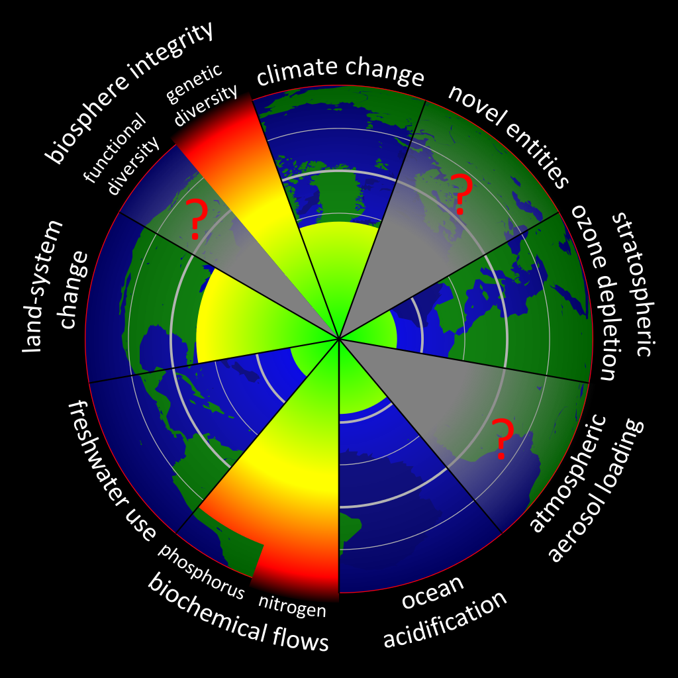
\includegraphics[width=0.6\linewidth]{figures/chap1/planetary_boundaries} 

}

\caption{The planetary boundaries (www.stockholmresilience.org)}\label{fig:f1}
\end{figure}

A more specific example of the plant-environment interactions is the
global carbon budget. We are currently facing this significant change in
biogeochemical cycling due to the rising fossil fuel emission over the
last 150 years. Figure \ref{fig:f2} represents the balance between
carbon sources (fossil carbon and land-use changes) and sinks (oceans,
land, and atmosphere). The more we emit, the more the Earth system is
capturing. Naturally, the emitted CO2 must go somewhere. Approximately
half of it is taken up by the ocean and the land (soil + vegetation)
sink. As stated earlier, roughly 25\% of the emitted CO2 is dissolved in
the ocean sink. The land sink is highly variable: land and soils are
very heterogeneous and difficult to model. Nevertheless, the land sink
has taken up more emissions in the past 60 years than it did before. The
atmosphere is responsible for most of the uptake. This takes us to a
question, frequently addressed by global vegetation models, about how
long these sinks will continue or not capture our increasing carbon
emissions. Note that there is an imbalance: there was more CO2 emitted
then absorbed. So, where did the surplus go? This is an active area of
research.

\begin{figure}

{\centering 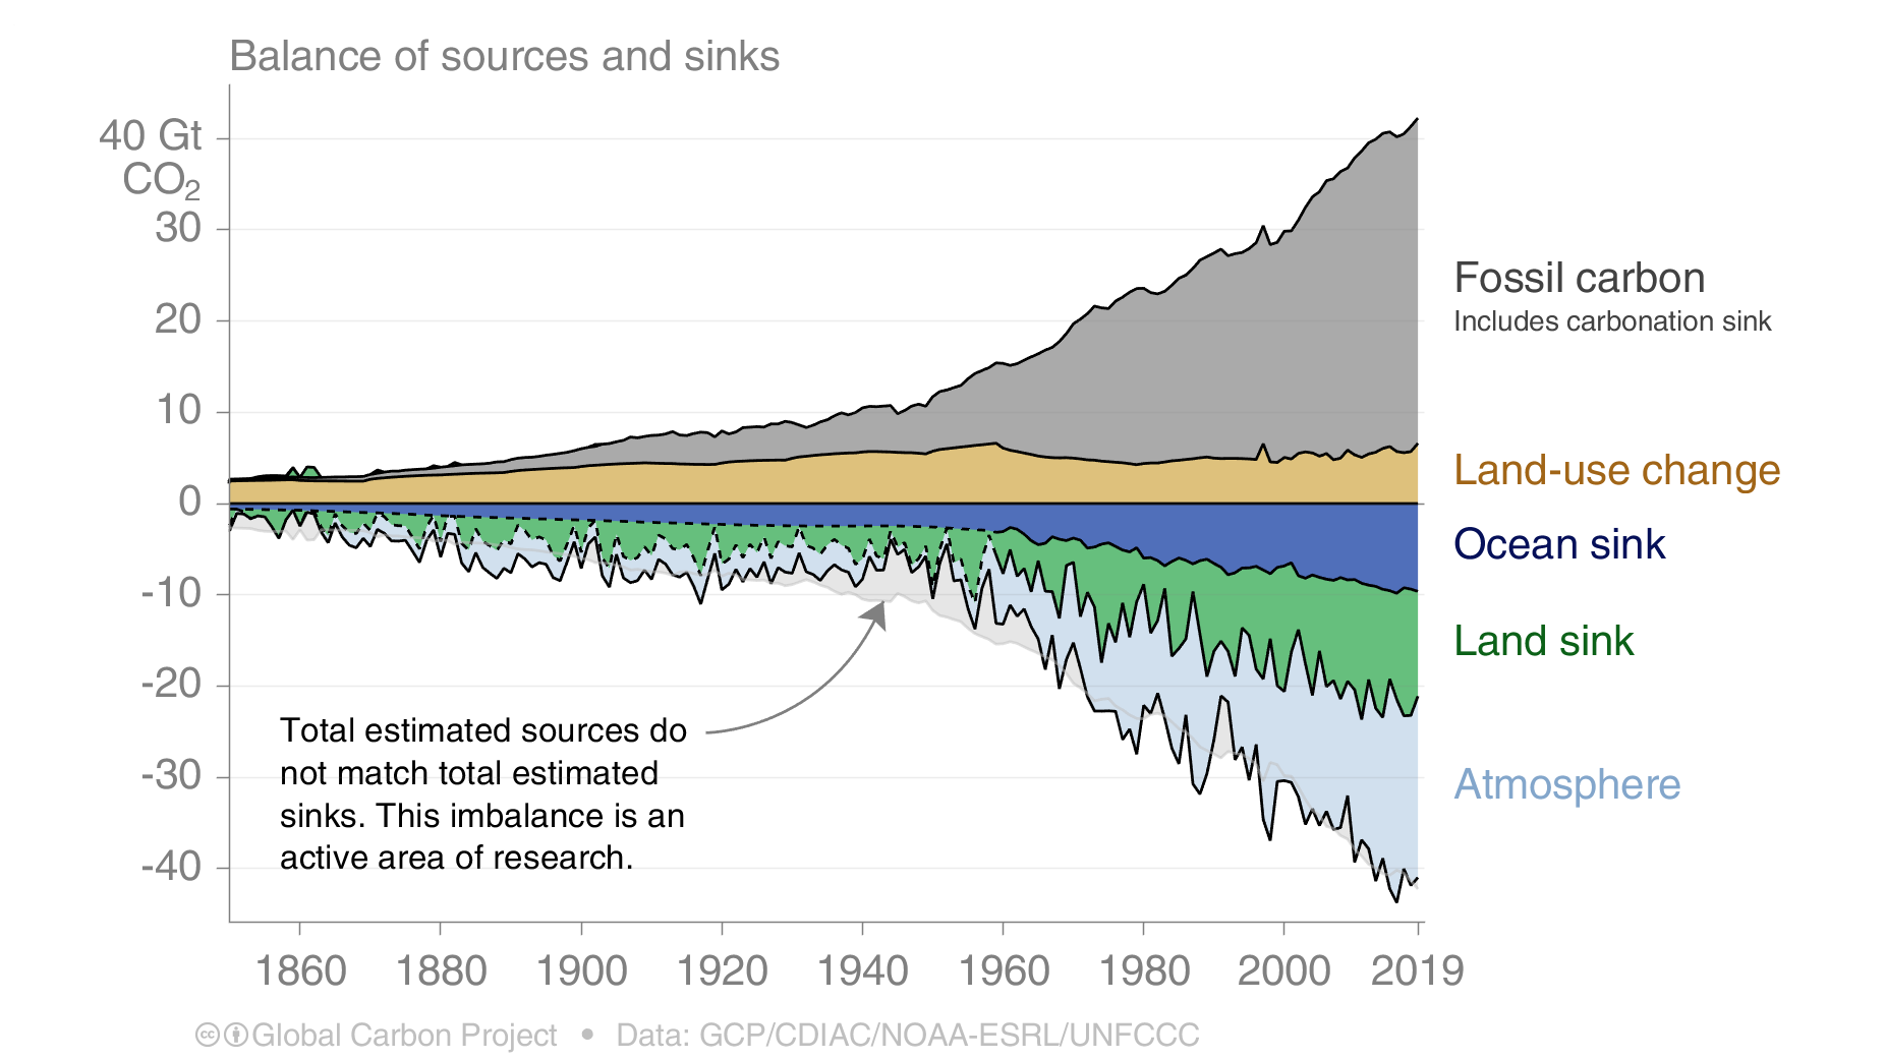
\includegraphics[width=0.8\linewidth]{figures/chap1/carbon_budget} 

}

\caption{The global carbon budget (www.globalcarbonproject.org)}\label{fig:f2}
\end{figure}

\textbf{Climate Models} predict how the long-term weather variation and
average weather will evolve. These models include an atmosphere, land
and ocean component (Figure \ref{fig:f3} top). The original climate
models focused on biophysics: energy and water balances, predicting
precipitation, radiation and fluxes between the three components. More
recently, climate models have evolved into \textbf{Earth System Models}
(ESM). ESM have a more complex concept because they represents more
processes (Figure \ref{fig:f3} bottom). Why? If you want to predict the
end of the century climate, we need to consider greenhouse gases and
thus the full carbon cycle. ESM are more complex but also more
realistic.

\begin{figure}

{\centering 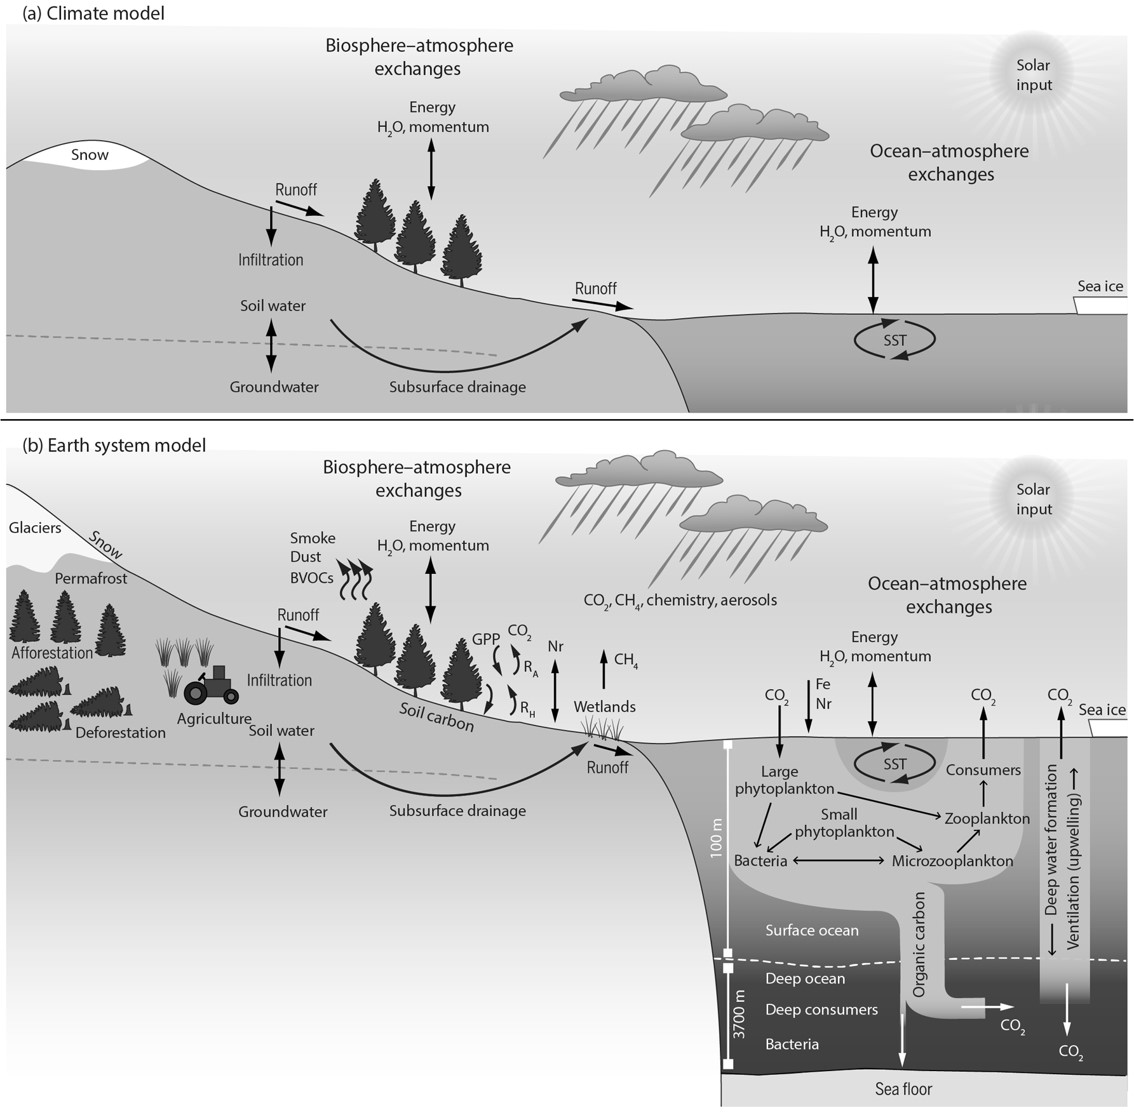
\includegraphics[width=0.7\linewidth]{figures/chap1/GCM_ESM} 

}

\caption{Scientific scope of (a) climate models and (b) earth system models. (Bonan 2019)}\label{fig:f3}
\end{figure}

Vegetation models are often the land component of an earth system model.
These `terrestrial biosphere models'(TBM) or `land surface models' (LSM)

\begin{itemize}
\tightlist
\item
  simulate \textbf{energy fluxes}: radiation, evapotranspiration and
  sensible heat fluxes between the land and the atmosphere. Depending on
  the vegetation type, the impacts are different.
\item
  simulate the \textbf{hydrology} and the \textbf{carbon cycle}.
\item
  simulate slower processes like \textbf{vegetation dynamics}: the
  succession of forest or \textbf{land use} and \textbf{urbanization}.
\end{itemize}

\begin{figure}

{\centering 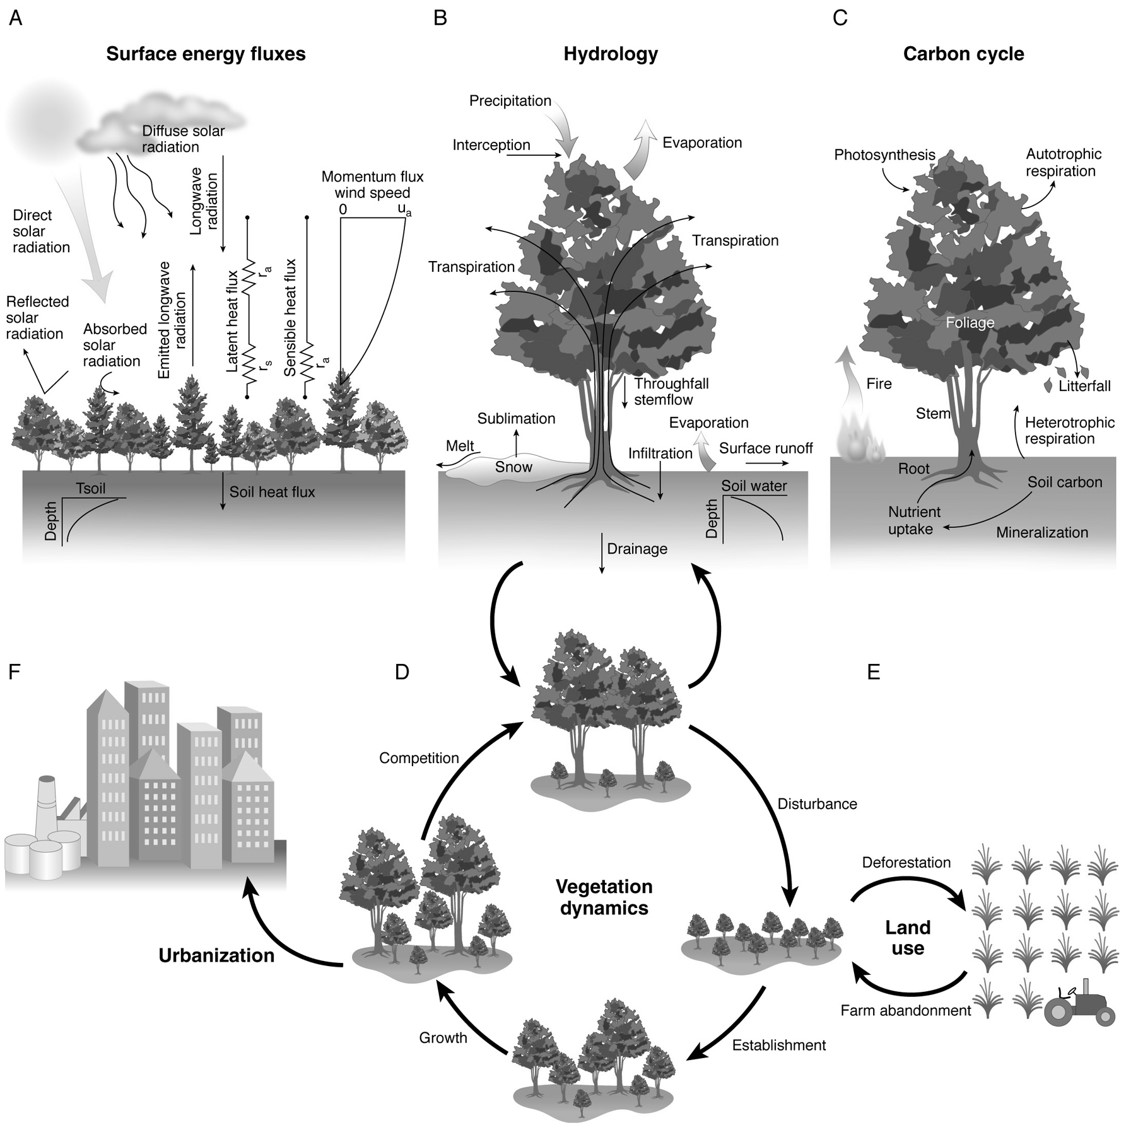
\includegraphics[width=0.8\linewidth]{figures/chap1/cycles_bonan} 

}

\caption{Scientific scope of terrestrial biosphere model. (Bonan 2019)}\label{fig:f4}
\end{figure}

The coupler is a system that links different models. For example the
terrestrial biosphere can be seen as the coupler between geochemistry
and hydrology. A coupler can be the link between more than two other
systems, so that a kind of satellite system is formed. The land model is
mostly seen as the coupler. This results in the fact that both fast and
slow processes depend on each other. The surface energy flux is an
example of a fast process since it varies over the course of one day
Vegetation dynamics on the other hand, is a slow process. Succession
does not happen overnight.

\section{Why do we need modelling?}\label{why-do-we-need-modelling}

Modelling has proven to be a essential tool:

\begin{itemize}
\tightlist
\item
  For \textbf{understanding}: we need good theoretical foundations
  (understand processes) to generalize knowledge and observations in
  space and time (upscaling). Studying the inaccuraies in models leads
  to the formulation of new hypotheses.
\item
  For \textbf{prediction}, how vegetation responds to expected changes
  (temperature or CO2) to develop management strategies and policies.
\item
  For \textbf{data integration}: a framework to bring together multiple
  data sources and to guide future data collection.
\end{itemize}

\section{Model types}\label{model-types}

How can we look at the different model types that exist (Table
\ref{table:example})? Models are to be placed in a continuum ranging
from empirical to process-based models. \textbf{Empirical models} are
based on data and correlations, not describing precisely the biophysical
processes --- \textbf{process-based models} describing the biophysical
processes and causal relations between the variables (Table
\ref{table:empiricial}). Most existing vegetation models are hybrid.

\begin{center}
\captionof{table}{Continuum of terrestrial biosphere/ecosystem models. (Bonan 2019)}
\label{table:example}

\begin{center}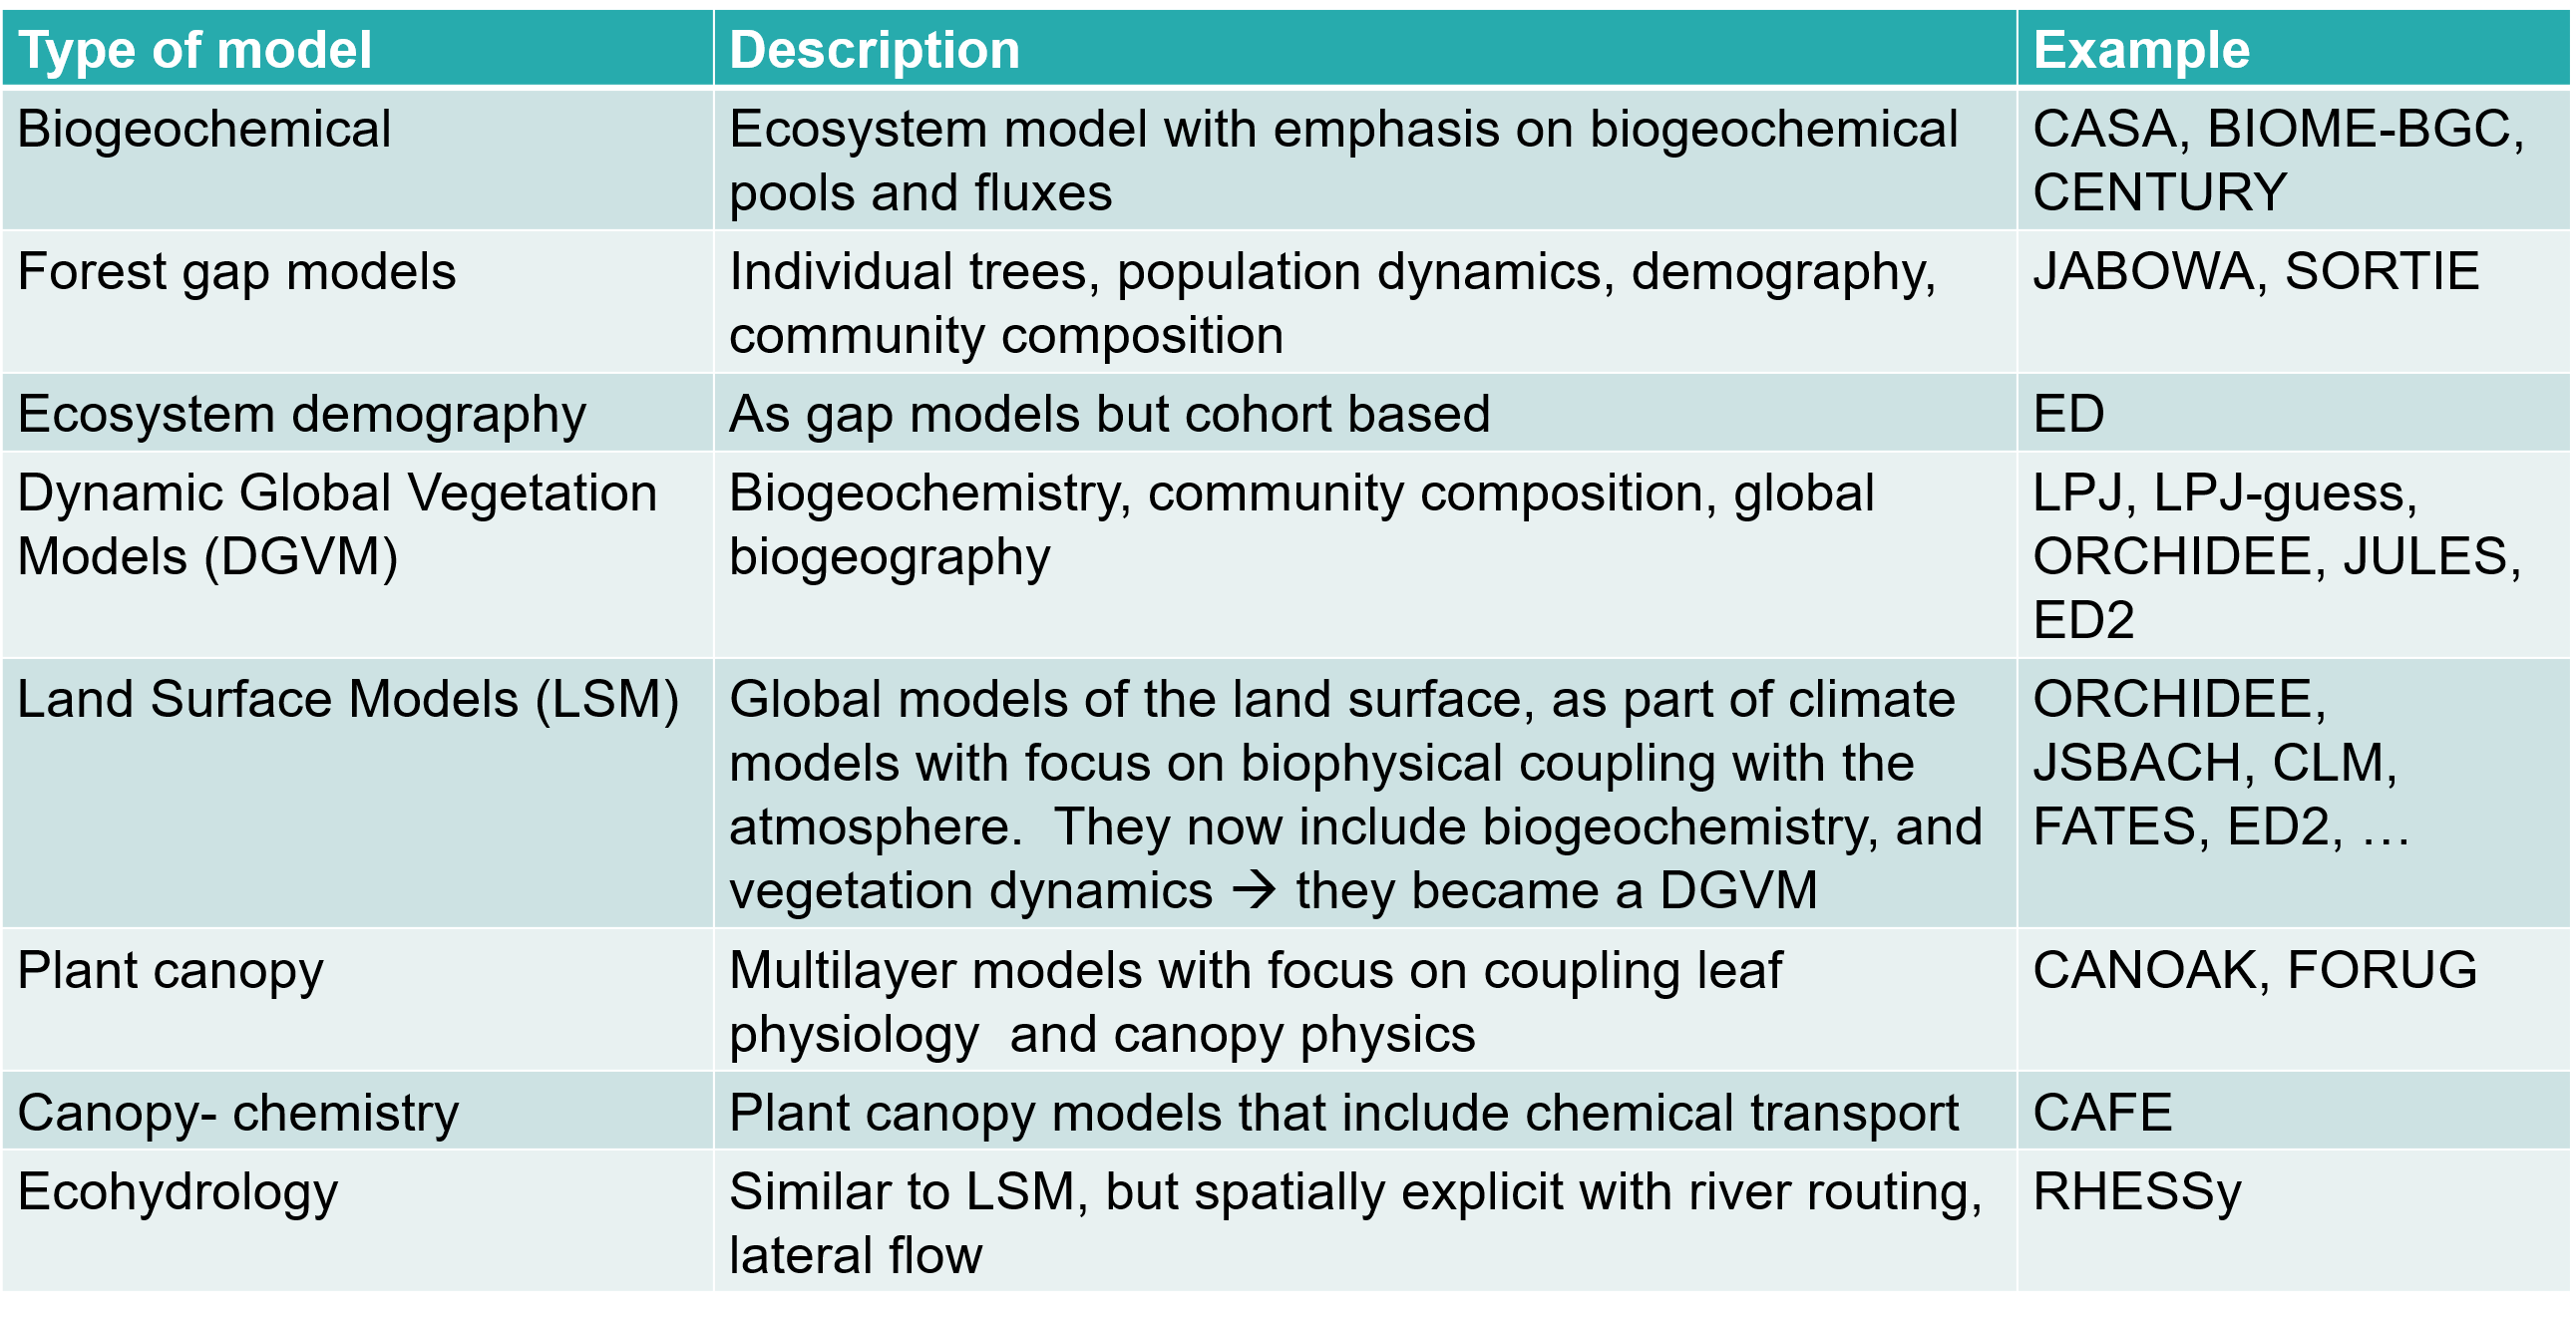
\includegraphics[width=0.8\linewidth]{figures/chap1/table_model_types} \end{center}
\end{center}

\begin{center}
\captionof{table}{Continuum of process-based versus empirical models. (Adams et al. 2013)}
\label{table:empiricial}

\begin{center}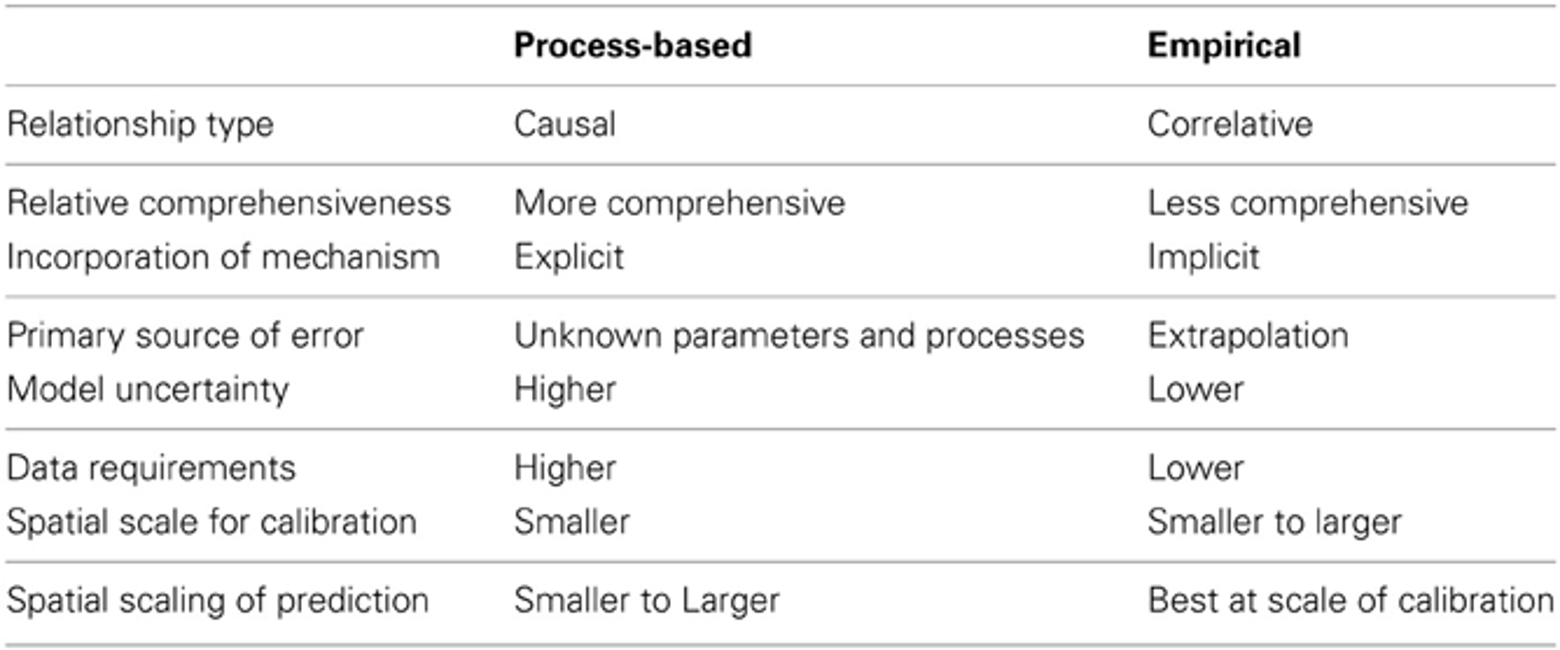
\includegraphics[width=0.8\linewidth]{figures/chap1/tables_PB_empirical} \end{center}
\end{center}

The model type depends on: - Purpose: will it be used for management
support, policy support, research. - Question: different people will be
interested in different questions (foresters, ecologists, policy
makers\ldots{}) - Scale: models that are to be applied for local use can
be much more detailed than worldwide models because data gathering is
much more straightforward on a small scale. Also the time-scale is of
importance: will the model be used for research about the past, the
present or the future?

\section{The history of vegetation
models}\label{the-history-of-vegetation-models}

The history of vegetation models is one that parallels that of the
computer. Computers made it possible to calculate much faster and much
more, which made them suitable for modelling. The first vegetation
models have emerged in the 1960s and 1970s.

One of the first models were the \textbf{box models} (1960); these
models describe the flow of mass and energy through boxes. These models
still exist in current biogeochemical models, where arrows represent the
fluxes between the pools. In parallel, \textbf{gap models} had emerged.
Gap models simulate the dynamics of the development of a gap in a forest
and the growth of plants in this gap. Gaps can be created by fallen
trees, by dead trees, \ldots{} . This kind of models are
individual-based and focused on population dynamics and the life cycle
of species: growth, regeneration and mortality while taking
environmental constraints in account. These models are the first models
that were ever used for upscaling: from tree level, to plot-level, to
landscape level. They were developed by forest scientists using forest
inventories to derive growth, regeneration, and mortality in response to
environmental variables. In 1973, the first model (MIAMI model by Lieth
(1973)) was developed to derive global net primary productivity (NPP),
relating NPP in an empirical way to climate variables (temperature) with
vegetation productivity. This was the first attempt to make a global
upscaling of a vegetation process. In the 1980s surged the first
\textbf{land surface models}. Land surface models are the models where
the other models start to integrate into, and evolved as such into --
\textbf{Terrestrial biosphere models} (see Figure \ref{fig:f7}), which
are now the state-of-the-art land components of ESMs. Vegetation
modelling therefore is a very interdisciplinary field because it
involves knowledge of different scientific fields, making it difficult
to find a common terminology. Global EMS are currently still not good to
simulate realistic vegetation dynamics.

\begin{figure}

{\centering 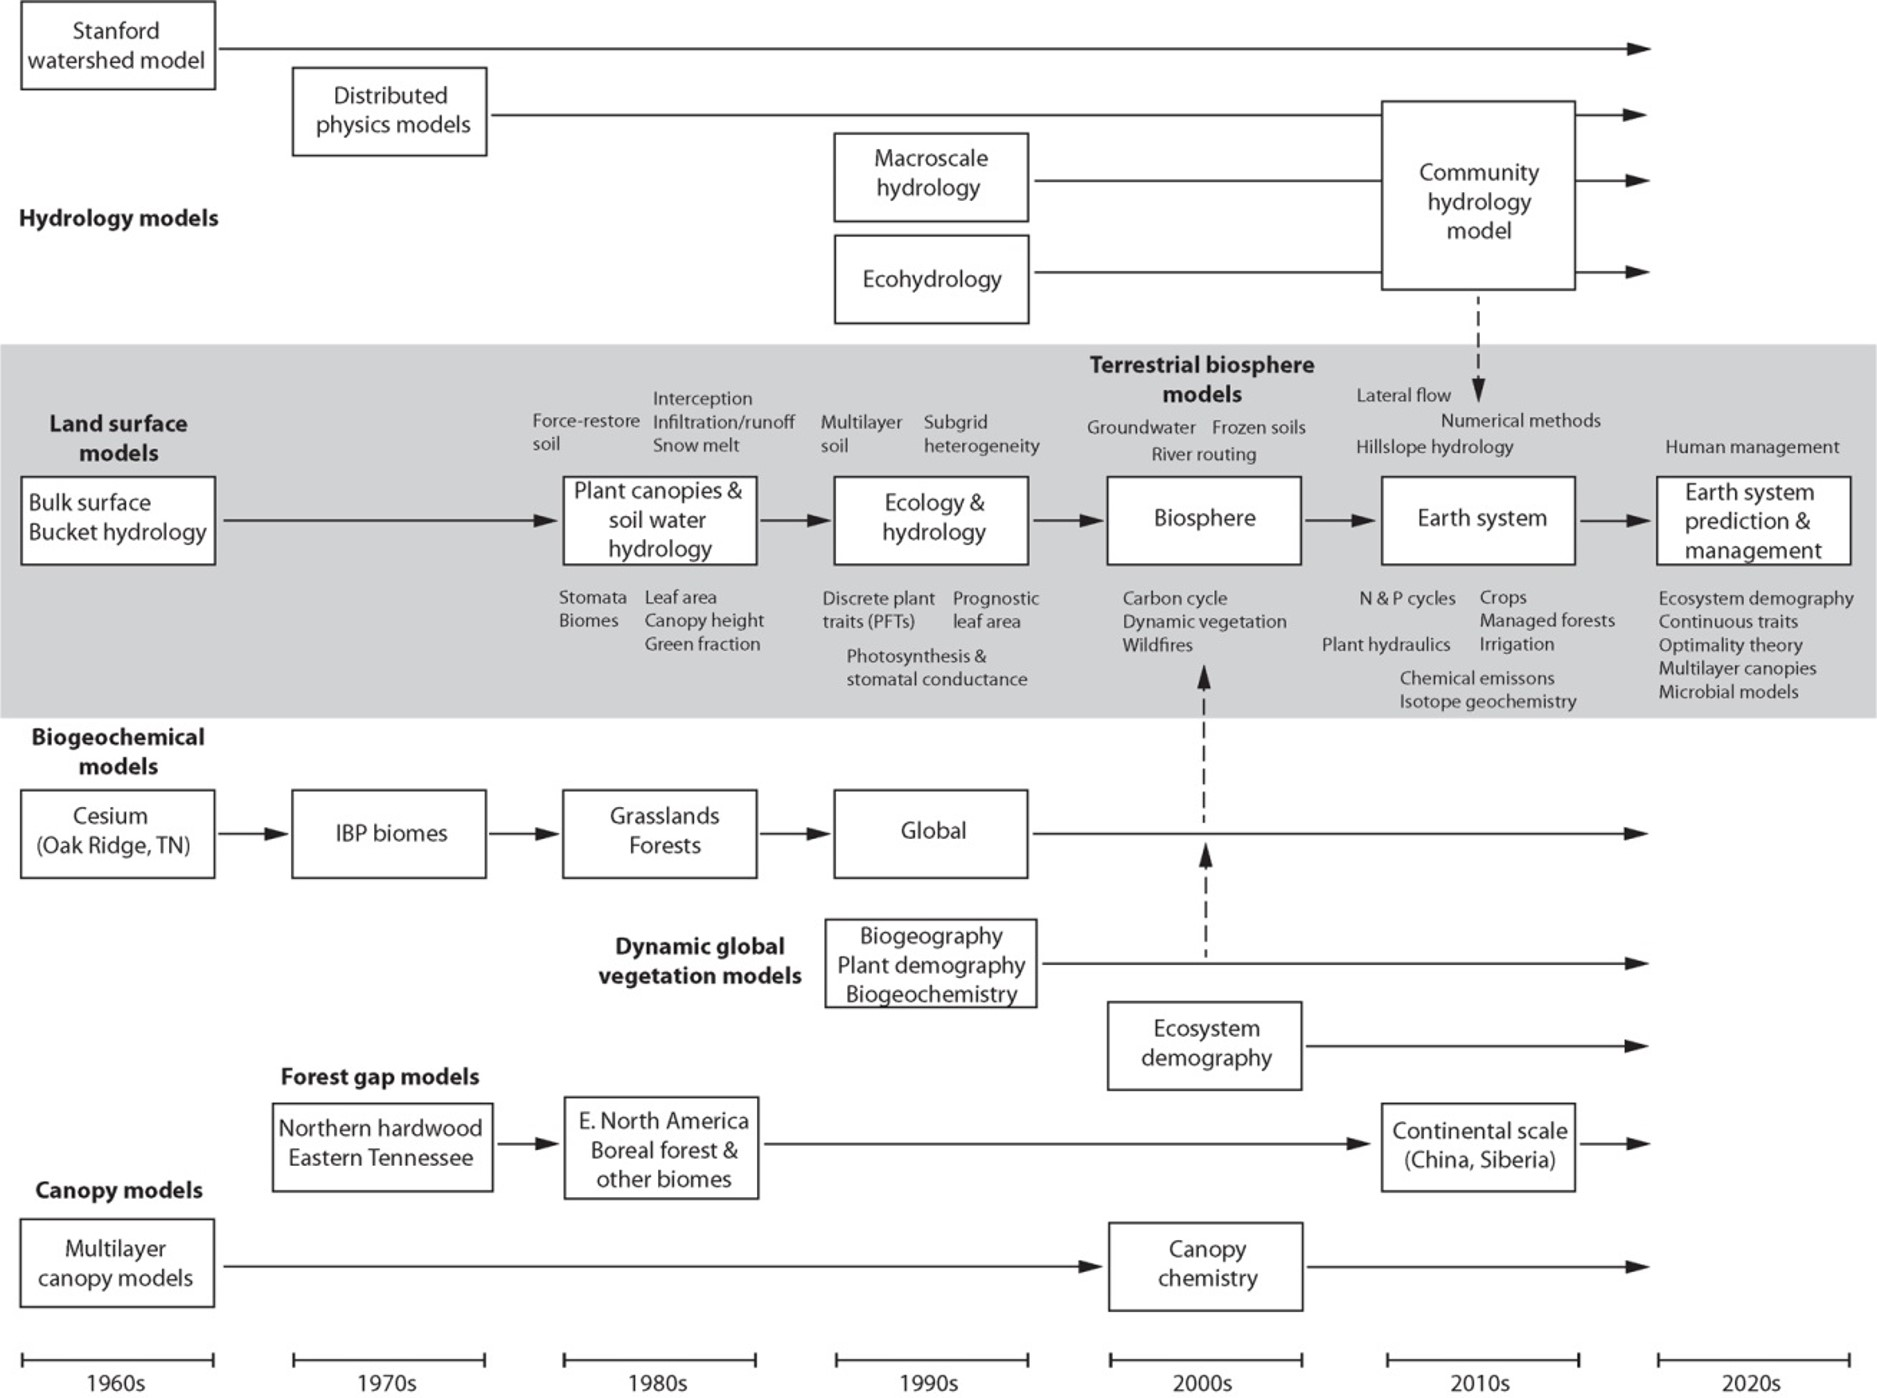
\includegraphics[width=0.8\linewidth]{figures/chap1/timeline} 

}

\caption{Timeline showing the parallel development of model types and the integration of model types into land surface models towards terrestrial biosphere models. (Bonan 2019)}\label{fig:f7}
\end{figure}

\section{Components of a model}\label{components-of-a-model}

What is a vegetation model? Two attempts for a definition:

\begin{itemize}
\tightlist
\item
  \textbf{Dynamic global vegetation models} (DGVMs) are powerful tools
  to project past, current and future vegetation patterns and associated
  biogeochemical cycles (Scheiter et al., 2013).
\item
  A \textbf{Dynamic Global Vegetation Model} (DGVM) is a computer
  program that simulates shifts in potential vegetation and its
  associated biogeochemical and hydrological cycles as a response to
  shifts in climate. DGVMs use time series of climate data and, given
  constraints of latitude, topography, and soil characteristics,
  simulate monthly or daily dynamics of ecosystem processes. DGVMs are
  used most often to simulate the effects of future climate change on
  natural vegetation and its carbon and water cycles (Wikipedia 2021).
\end{itemize}

\begin{center}
\captionof{table}{Definition of key model components and examples for a typical TBM}
\label{table:components}

\begin{center}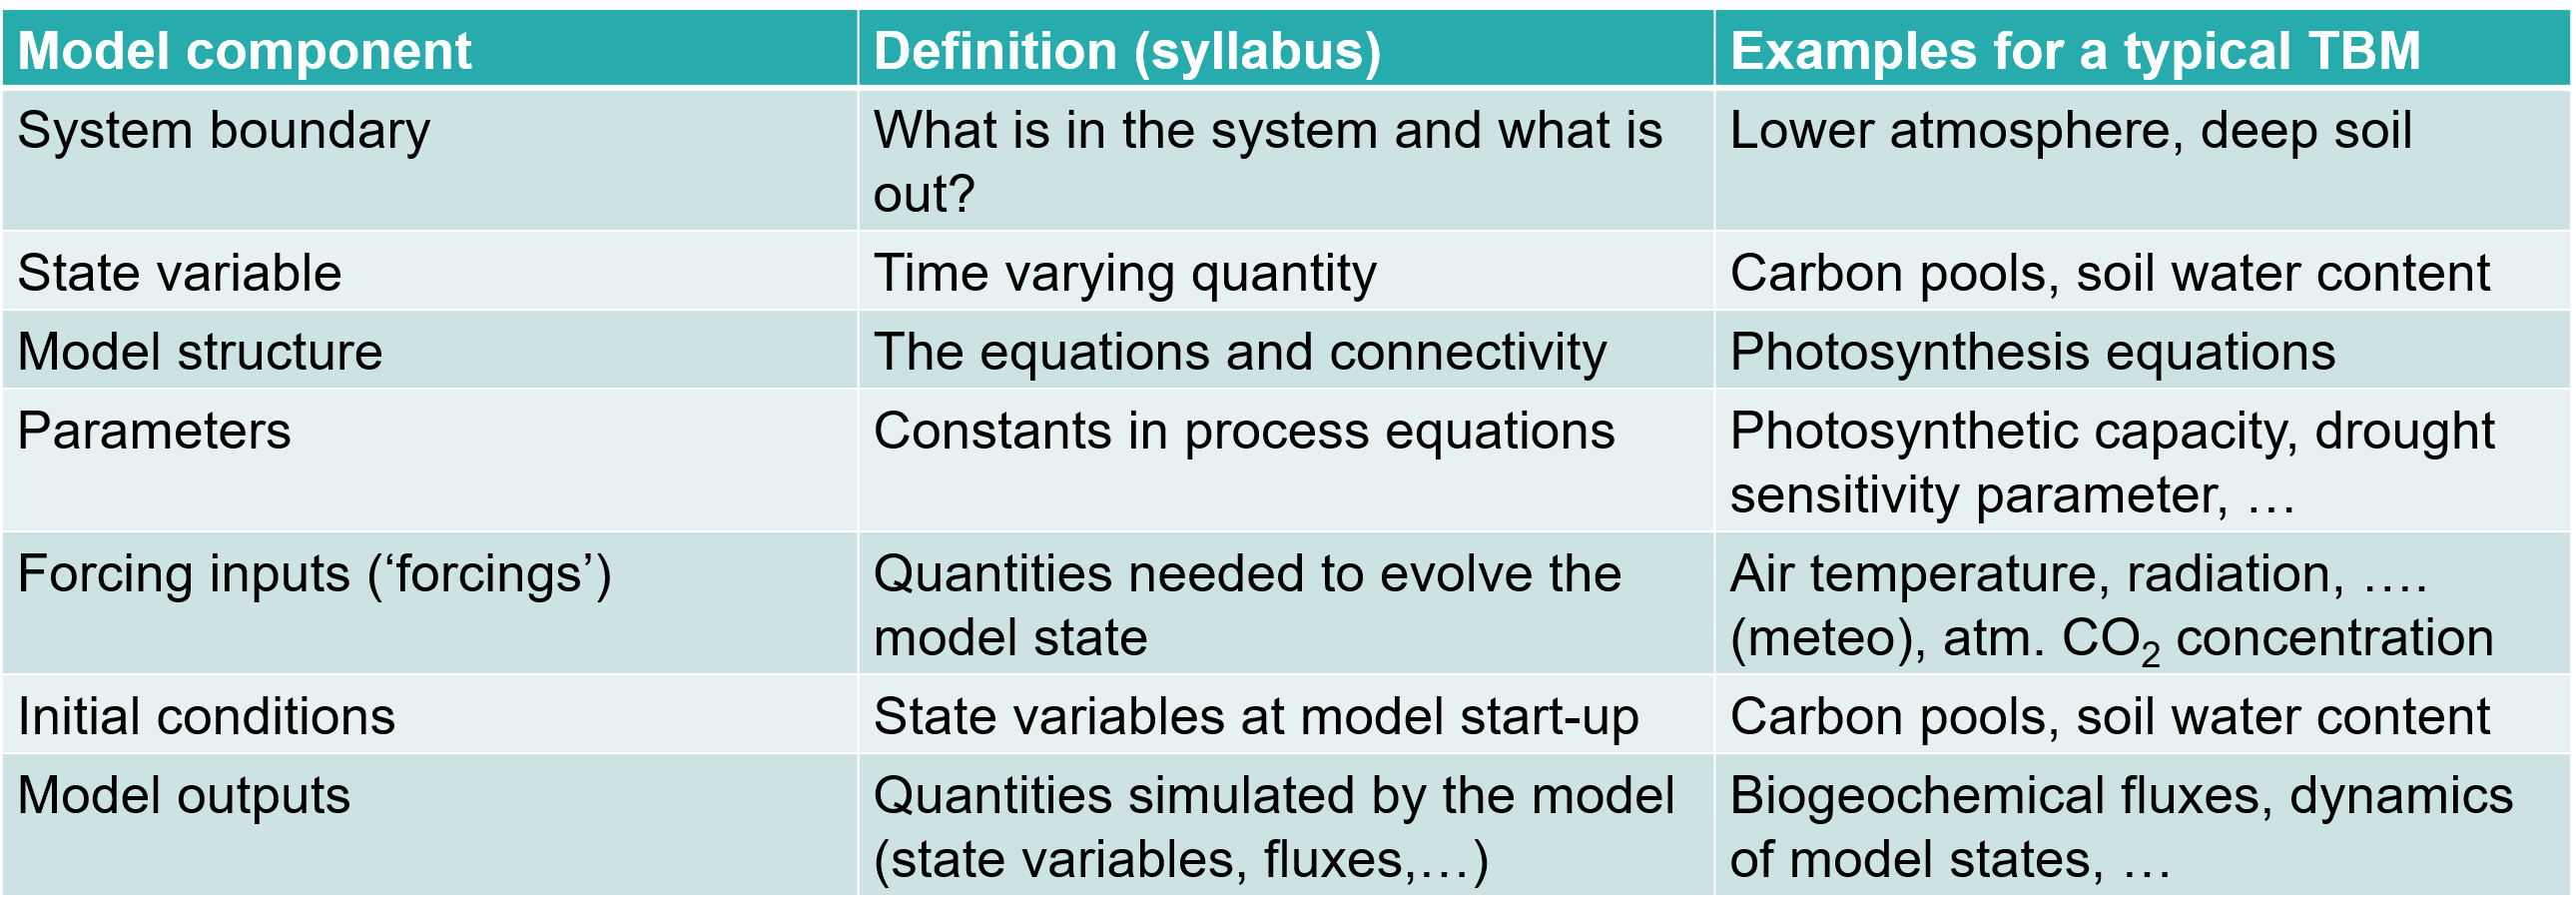
\includegraphics[width=0.9\linewidth]{figures/chap1/table_components} \end{center}
\end{center}

\subsection{Processes}\label{processes}

They are a key component because we are focusing on process-based models
in this course. There is a long list of processes (energy, water,
turbulent transport, canopy scaling, carbon, nitrogen, trace gasses,
demography,\ldots{}) that the models integrate, especially the more
complex ones. These processes will be discussed in detail in the
following theory chapters and we will mainly focus on how to translate
them into equations.

\subsection{Equations}\label{equations}

These are the mathematical representations of the processes. However,
there are important constraints to insert equations into a vegetation
model, such as the specific time scale at which a process operates. For
example, it makes little sense to resolve the equation for forest
composition (succession) on a daily calculation time step. This is a
prolonged process with an extremely low variance between consecutive
days. The solution for the equation for photosynthesis, on the other
hand, varies significantly throughout the day and between consecutive
days (cloudy day vs sunny day).

There are three types of equations within vegetation models: -
\textbf{prognostic equations}: time derivatives of differential
equations -- they calculate the state's change over time -
\textbf{conservation equations}: equations describing the conservation
of mass and energy - \textbf{diagnostic equations}: linking multiple
variables independent from the time.

Often there is no analytical solution of the equations describing
on-linear processes in biological systems; therefore, we must use
numerical methods to solve the equations.

\subsection{Parameters}\label{parameters}

These are the constants in the model. Some parameters are highly
uncertain because we cannot measure them very well at the relevant
scale. For example, we can make reliable measurements of the
photosynthetic capacity of a single leaf. However, upscaling this
parameter so that it is applicable for a forest or multiple PFTs (=
plant functional types) induces uncertainty. The more parameters a model
uses, the more uncertainties that are to be taken into account.

\subsection{Time Steps}\label{time-steps}

Vegetation models run at multiple timescales (combining processes that
are resolved at multiple timescales). Models present fast processes,
which are calculated every hour (e.g.~photosynthesis and energy
balance), intermediate processes calculated daily (e.g.~carbon
allocation and growth) and slow processes in order of years
(e.g.~mortality) (Fig.6).

\begin{figure}

{\centering 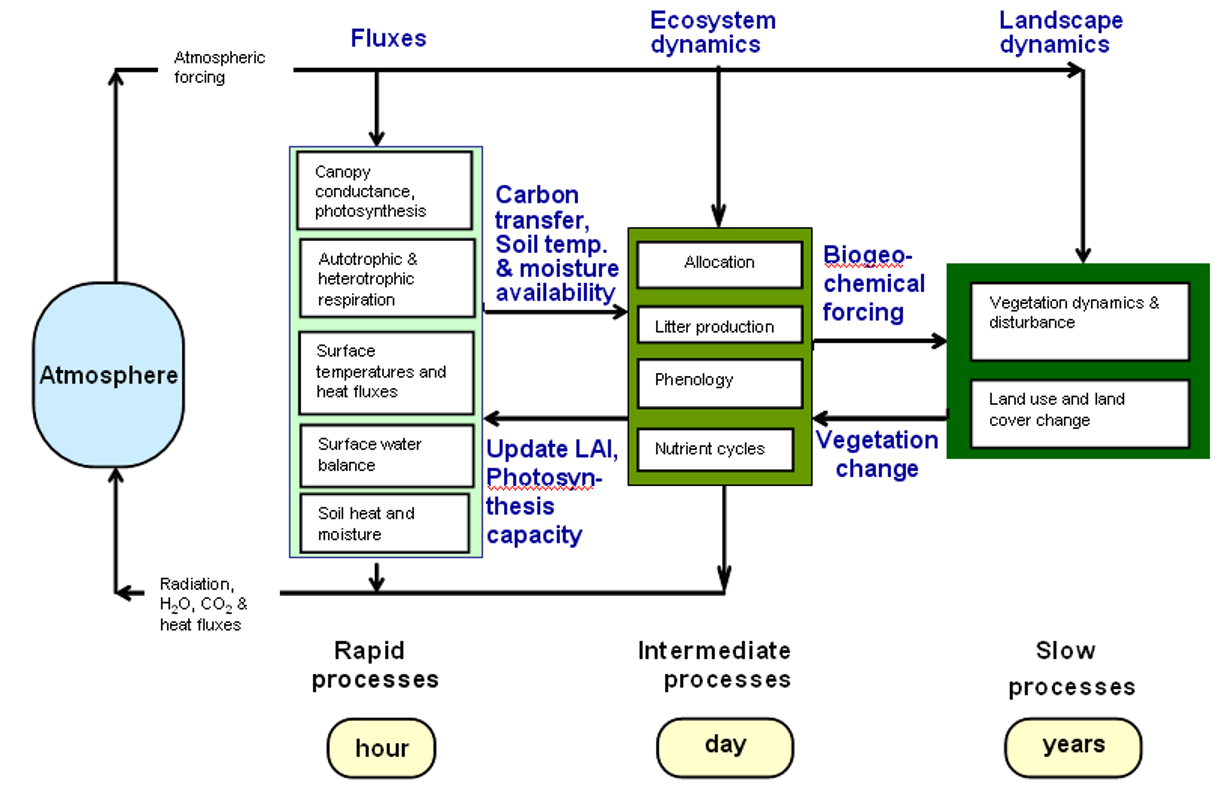
\includegraphics[width=0.8\linewidth]{figures/chap1/time_steps} 

}

\caption{Structure of a vegatation model indicating the different time steps at which each process is simulated (Williams et al. 2009)}\label{fig:f9}
\end{figure}

\subsection{Spatial structure}\label{spatial-structure}

The division of space in voxels, layers or grid cells and its resolution
determines how many times we repeat our calculations in space. Global
vegetation models have a typical spatial grid of 100km or even more and
divide the landscape into patches. In each patch, they simulate the
vegetation (forest, savannas, grassland\ldots{}). Models also have a
horizontal grid or horizontal layering: some models consider multiple
soil layers. The same is true for above ground layers, where some models
divide the canopy into multiple layers (Figure \ref{fig:f10}). For
example, the Ecosystem Demography Model (ED2.2) divides the forest into
multiple grid cells where the same meteorological conditions apply
within each grid cell. Then within each cell, this model has different
sites with different soils. Each site is divided into multiple patches
(forests with a similar disturbance history). For each patch, the model
simulates multiple cohorts of trees where size and plant functional
types play a role (Figure \ref{fig:f11}).

\begin{figure}

{\centering 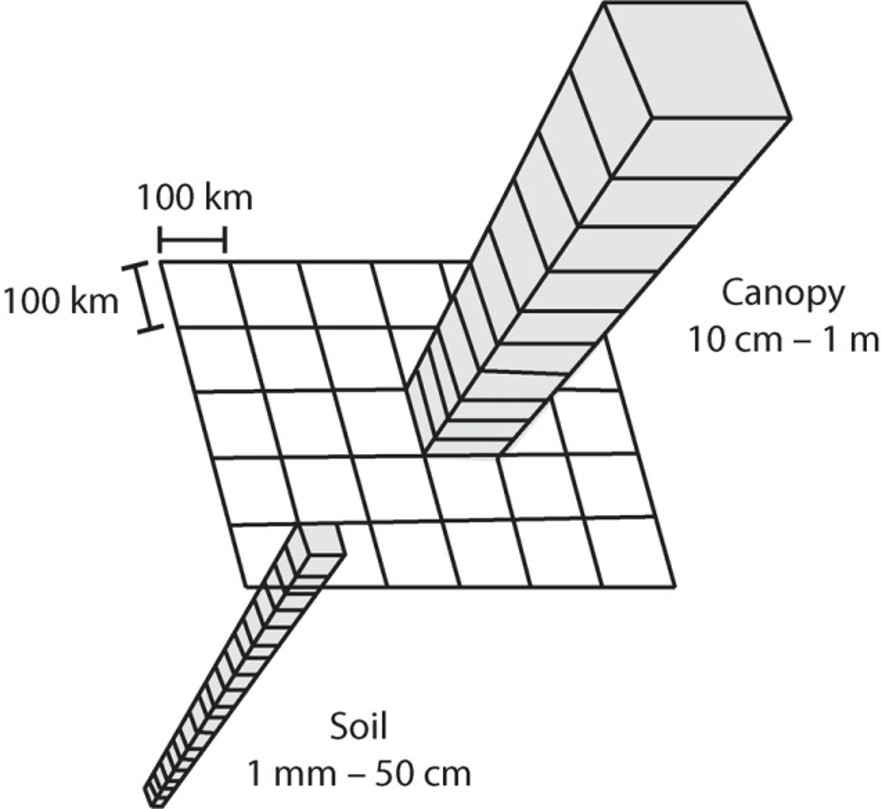
\includegraphics[width=0.5\linewidth]{figures/chap1/grid_vert_hor} 

}

\caption{Three dimensional grid of a TBM structured in terms of longitude x latitude x level. The number of soil and canopy layers and the geographical resolution is model dependent, (Bonan 2019)}\label{fig:f10}
\end{figure}

\begin{figure}

{\centering 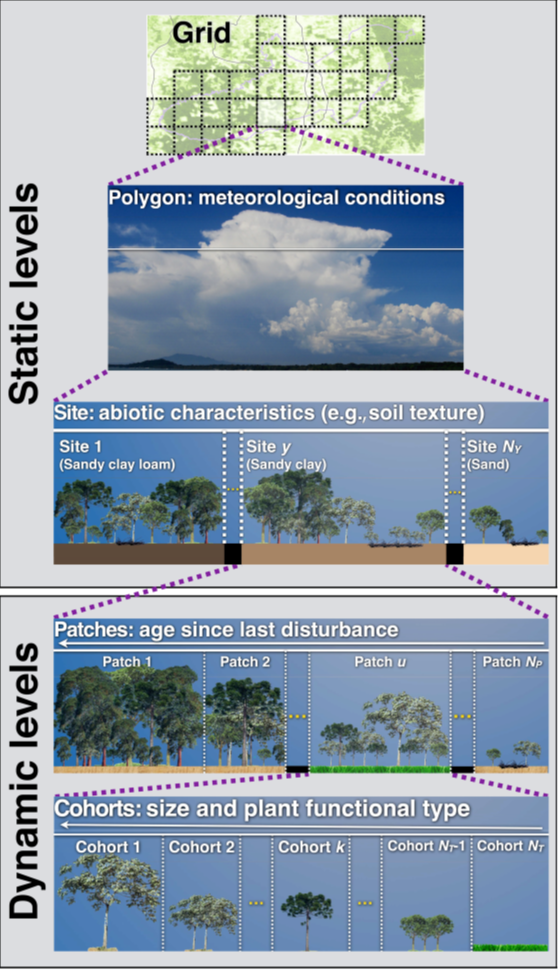
\includegraphics[width=0.7\linewidth]{figures/chap1/grid_ED2} 

}

\caption{Example: the spatial multi-level grid structure of of the ED2 vegetation model (Longo et al. 2019)}\label{fig:f11}
\end{figure}

\subsection{Model code, complexity and
uncertainty}\label{model-code-complexity-and-uncertainty}

There is a gap between equations and how the are implemented in the
actual model code. Also, a specific process can be implemented into an
equation in various ways. Usually, large models also contain a
``technical debt'', which means over the years, multiple modelers have
continued working on models and added code lines, but at some point, the
code is so large that none of the developers still knows the entire
code, resulting in persistent bugs or overlooked assumptions.

Models are always a simplification of the real world, but they tend to
become overly complex.

More complex models (adding more processes) become more realistic, but
we also add more sources of uncertainty. Therefore, we should choose our
model carefully based on the research question we want to adress.

\subsection{Data}\label{data}

It is not possible to develop models without data. In general, the more
data (multiple data sources), the better.

\section{Modelling workflow and structure of the
course}\label{modelling-workflow-and-structure-of-the-course}

Vegetation modelling is a multidisciplinary field. This course will
mainly focus on the mathematical formulation of processes and
translating these equations into a working model.

\begin{figure}

{\centering 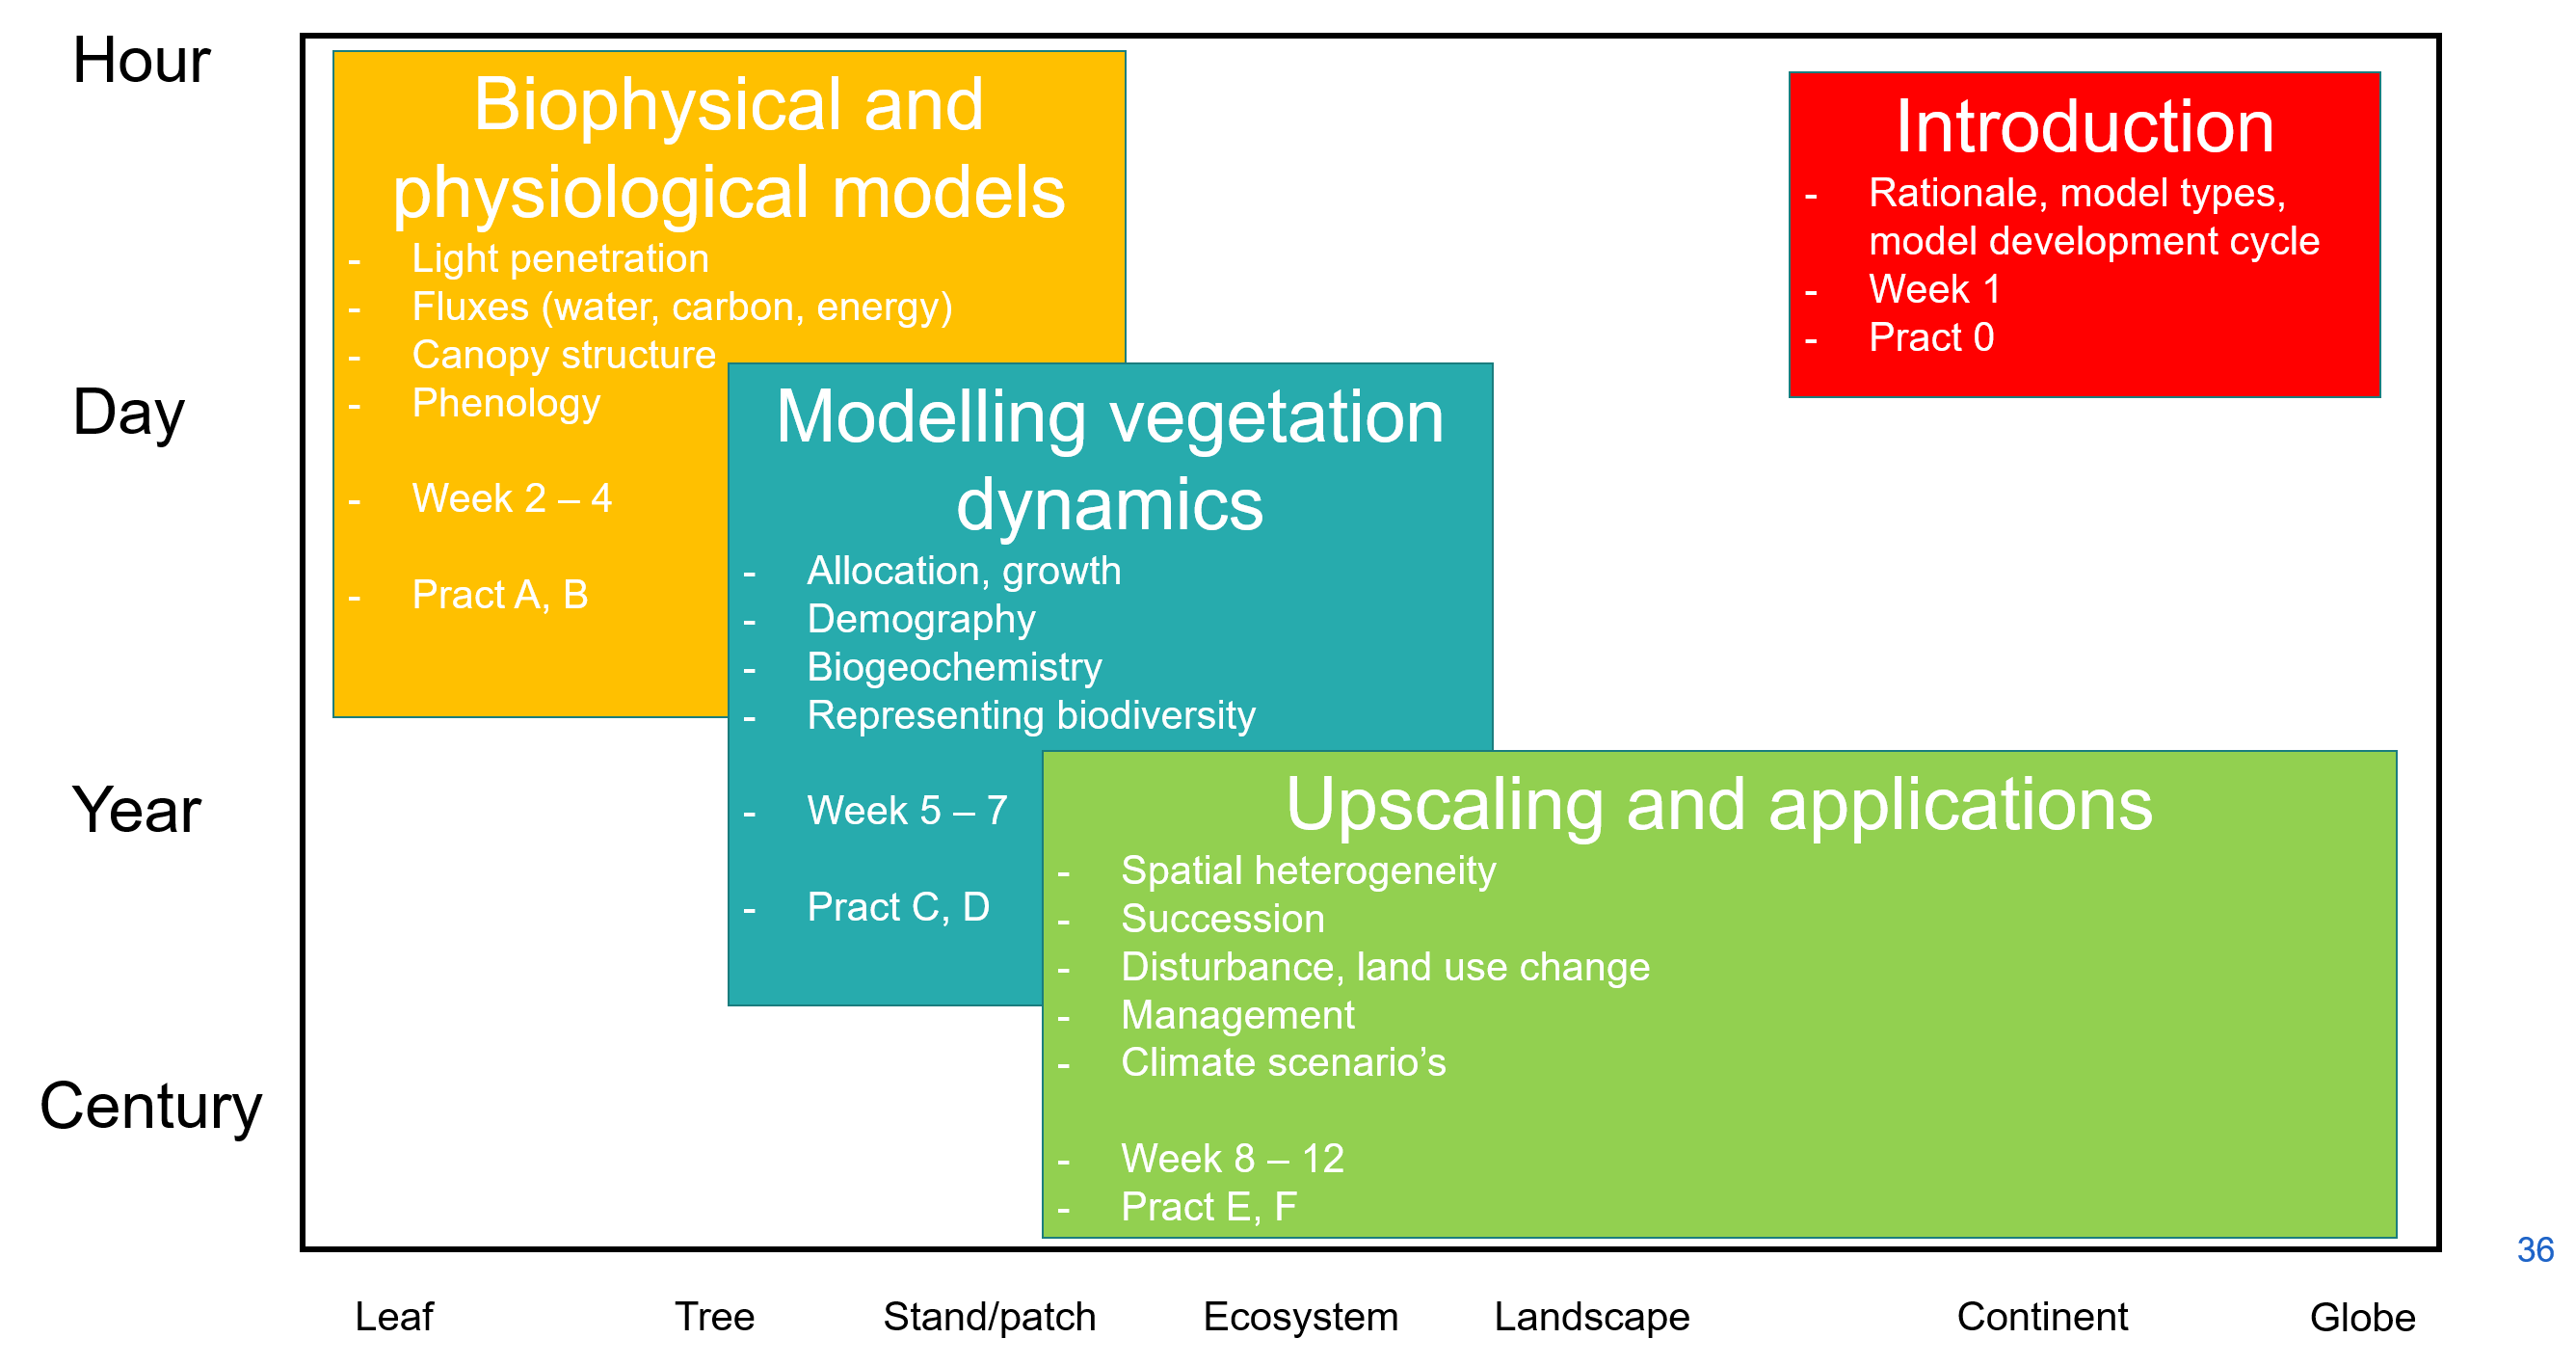
\includegraphics[width=0.9\linewidth]{figures/chap1/course_overview} 

}

\caption{Progression through spatial and temporal scales throughout this course}\label{fig:f12}
\end{figure}

The construction of a model is a continuous process -- a model is never
finished. As Figure 10 shows us, we start by describing our system in
the form of equations, then running the computer program to characterize
the model, perform parameter estimation and interpretation, and then
apply it to other locations and validate against independent data.

\begin{figure}

{\centering 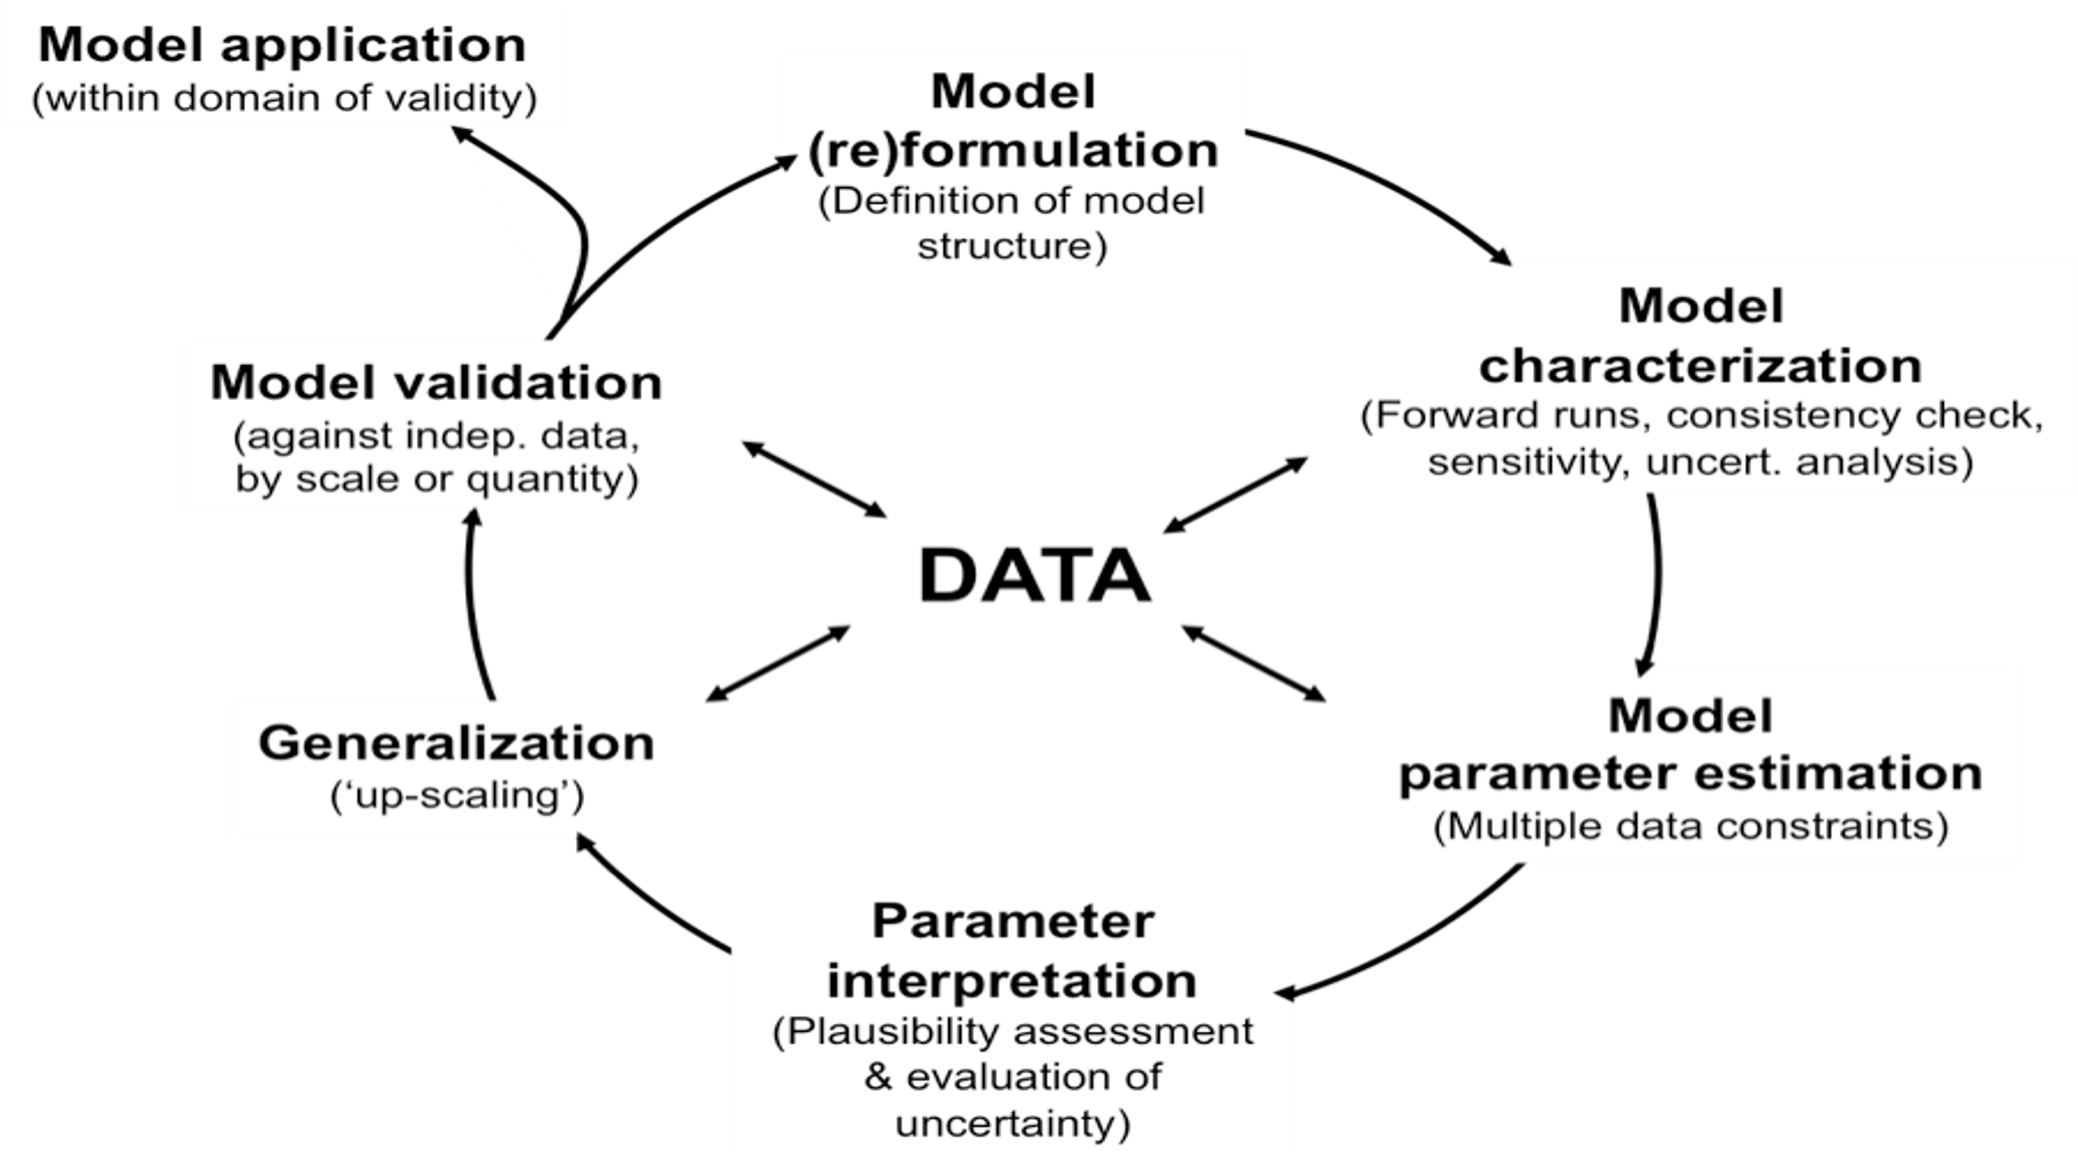
\includegraphics[width=0.8\linewidth]{figures/chap1/williams_fusion} 

}

\caption{Model data fusion in every step of the model development cycle (Williams et al. 2009)}\label{fig:f13}
\end{figure}

\begin{figure}

{\centering 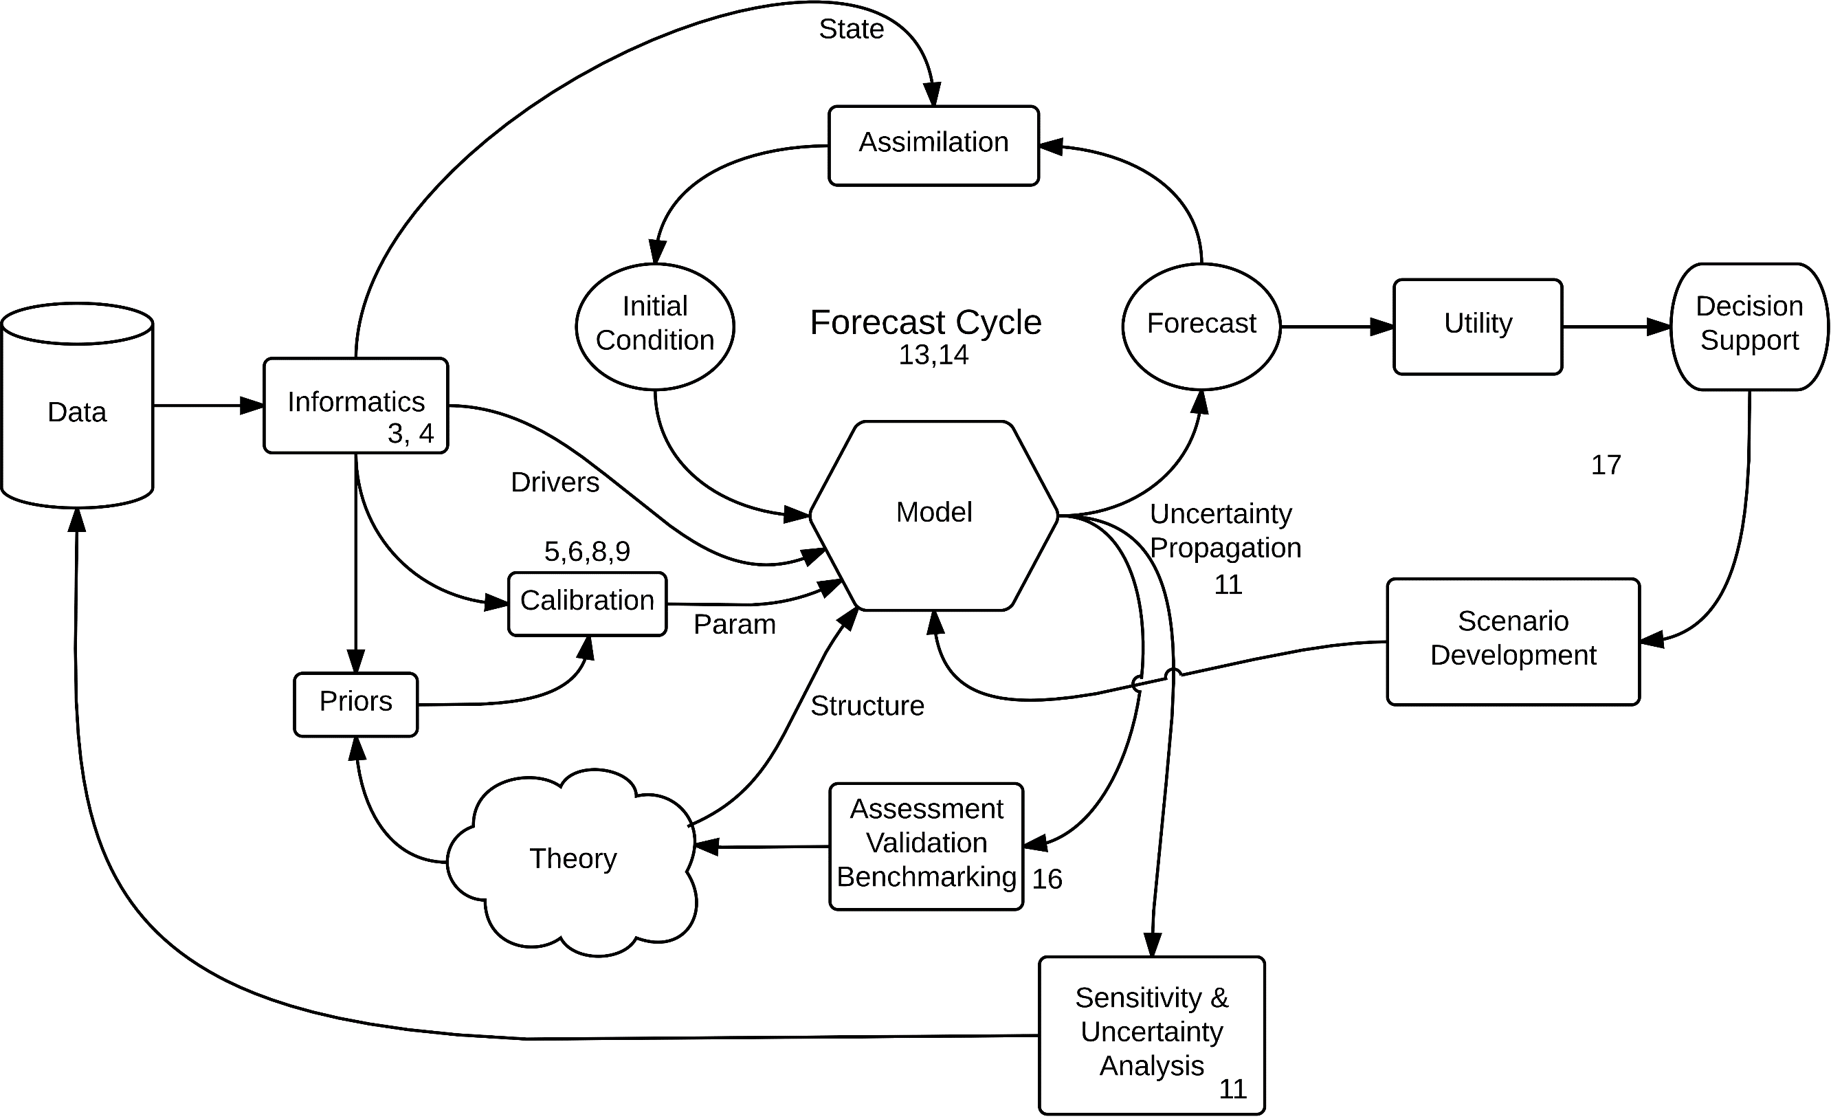
\includegraphics[width=0.8\linewidth]{figures/chap1/dietze_workflow} 

}

\caption{Methodological workflow of model data fusion (Dietze: Ecological Forecasting)}\label{fig:f14}
\end{figure}

\part{Biophysical and physiological
models}\label{part-biophysical-and-physiological-models}

\chapter{Modelling plant basic
processes}\label{modelling-plant-basic-processes}

\chaptermark{photsynthesis}

\textbf{For all processes, we provide an overview of existing models and
approaches and we will detail only one of them for the practical course.
This also apply for the other chapters, the idea of the course is to be
more conceptual about how we model vegetation and the different
applications and assumptions.}

\section{Photosynthesis models}\label{photosynthesis-models}

\subsection{Refreshing the basic
knowledge}\label{refreshing-the-basic-knowledge}

\begin{figure}

{\centering 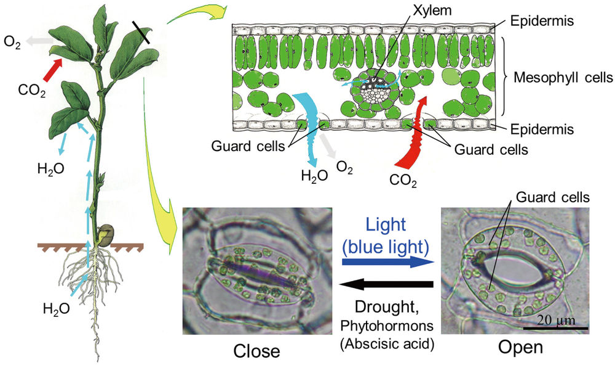
\includegraphics[width=0.8\linewidth]{figures/chap2/leaf_level_processes} 

}

\caption{Leaf level processes transpiration and photosysnthesis are strongy interlinked and both regulated by stomatal conductance}\label{fig:f21}
\end{figure}

\begin{figure}

{\centering 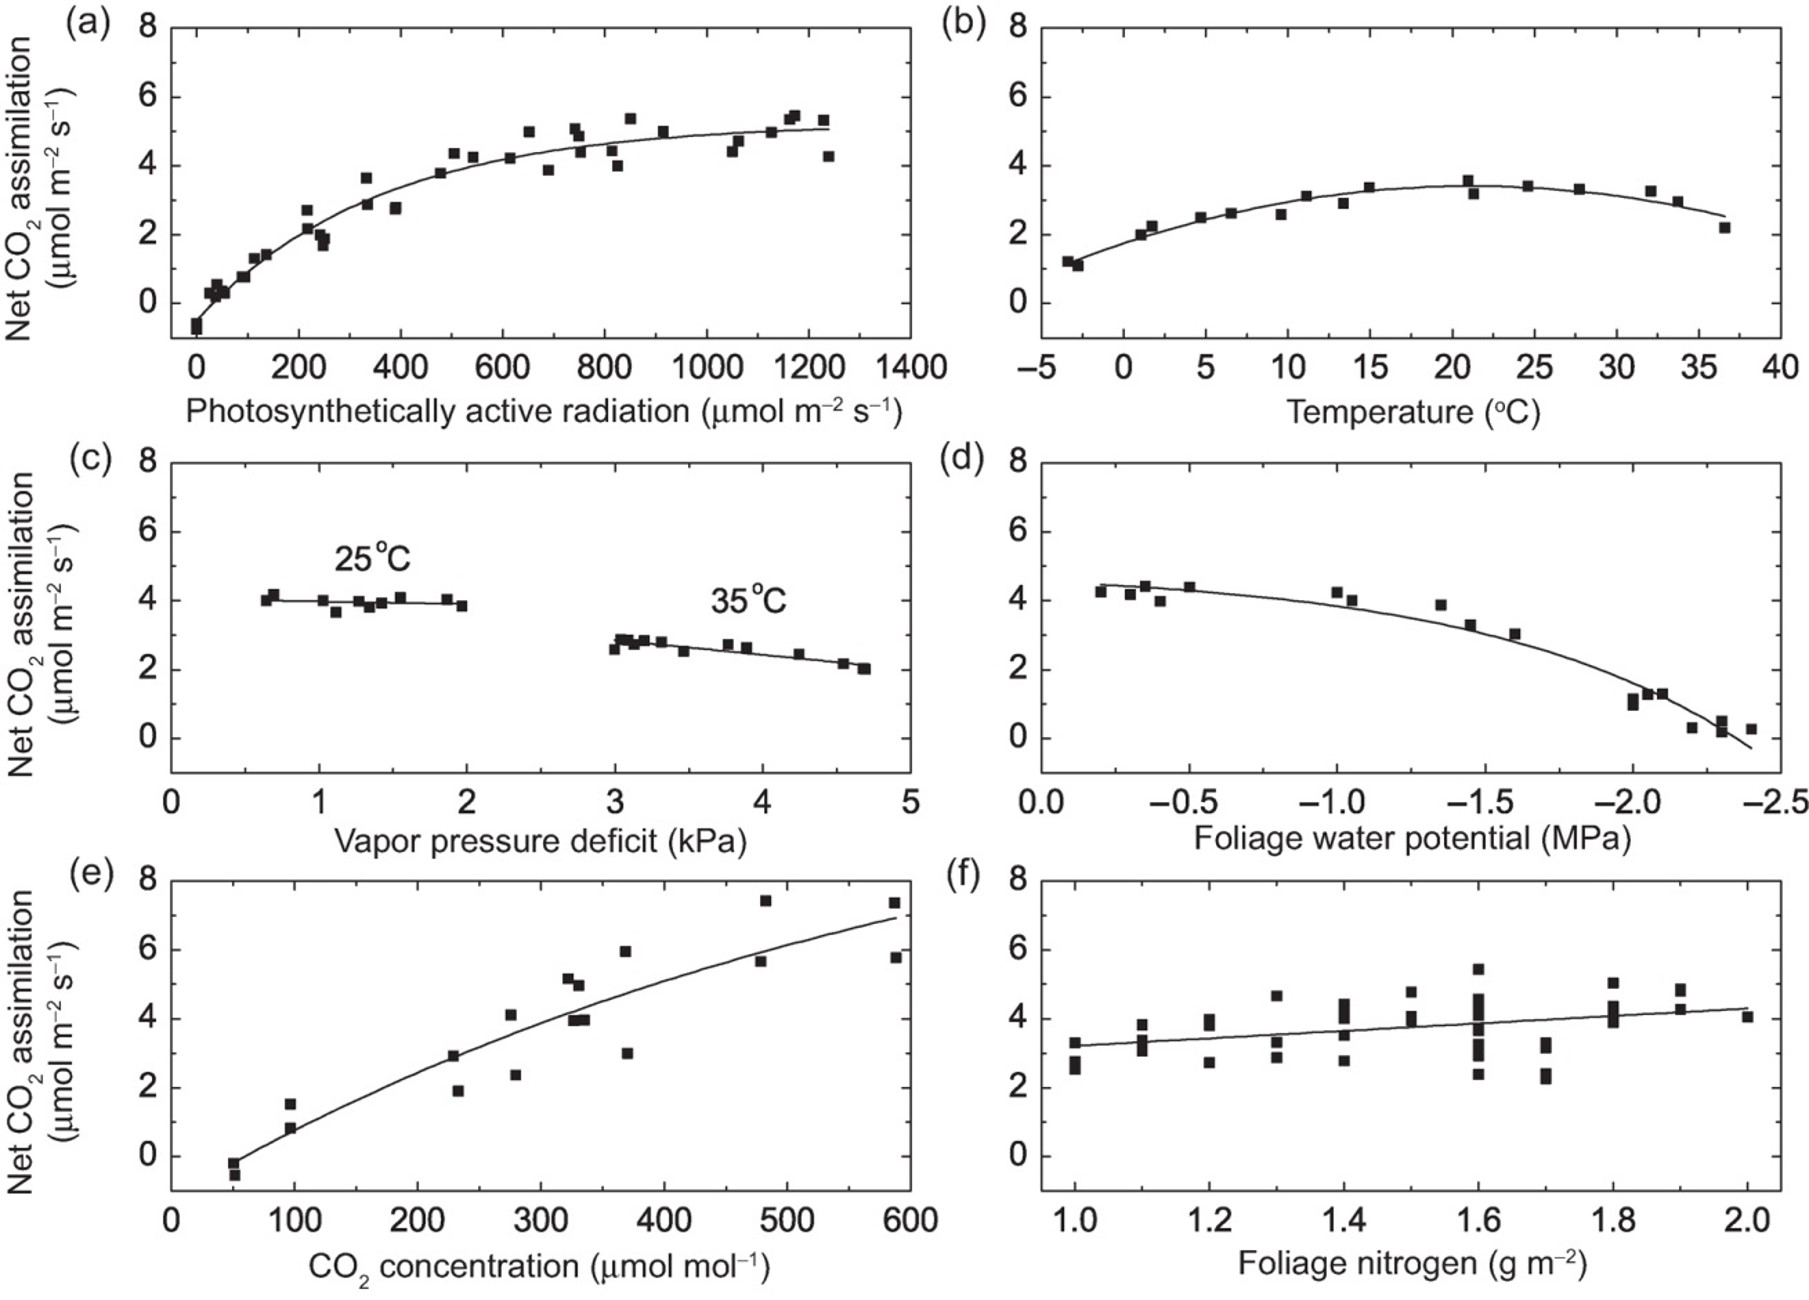
\includegraphics[width=0.8\linewidth]{figures/chap2/photosynthesis_obs} 

}

\caption{Photosynthesis in relation to (a) photosynthetically active radiation,(b) temperature, (c) vapor pressure deficit at 25°C and 35°C,(d) foliage water potential, (e) ambient CO2 concentration, and (f) foliage water potential for jack pine trees (Pinus banksiana). Bonan (2019)}\label{fig:f22}
\end{figure}

\begin{figure}

{\centering 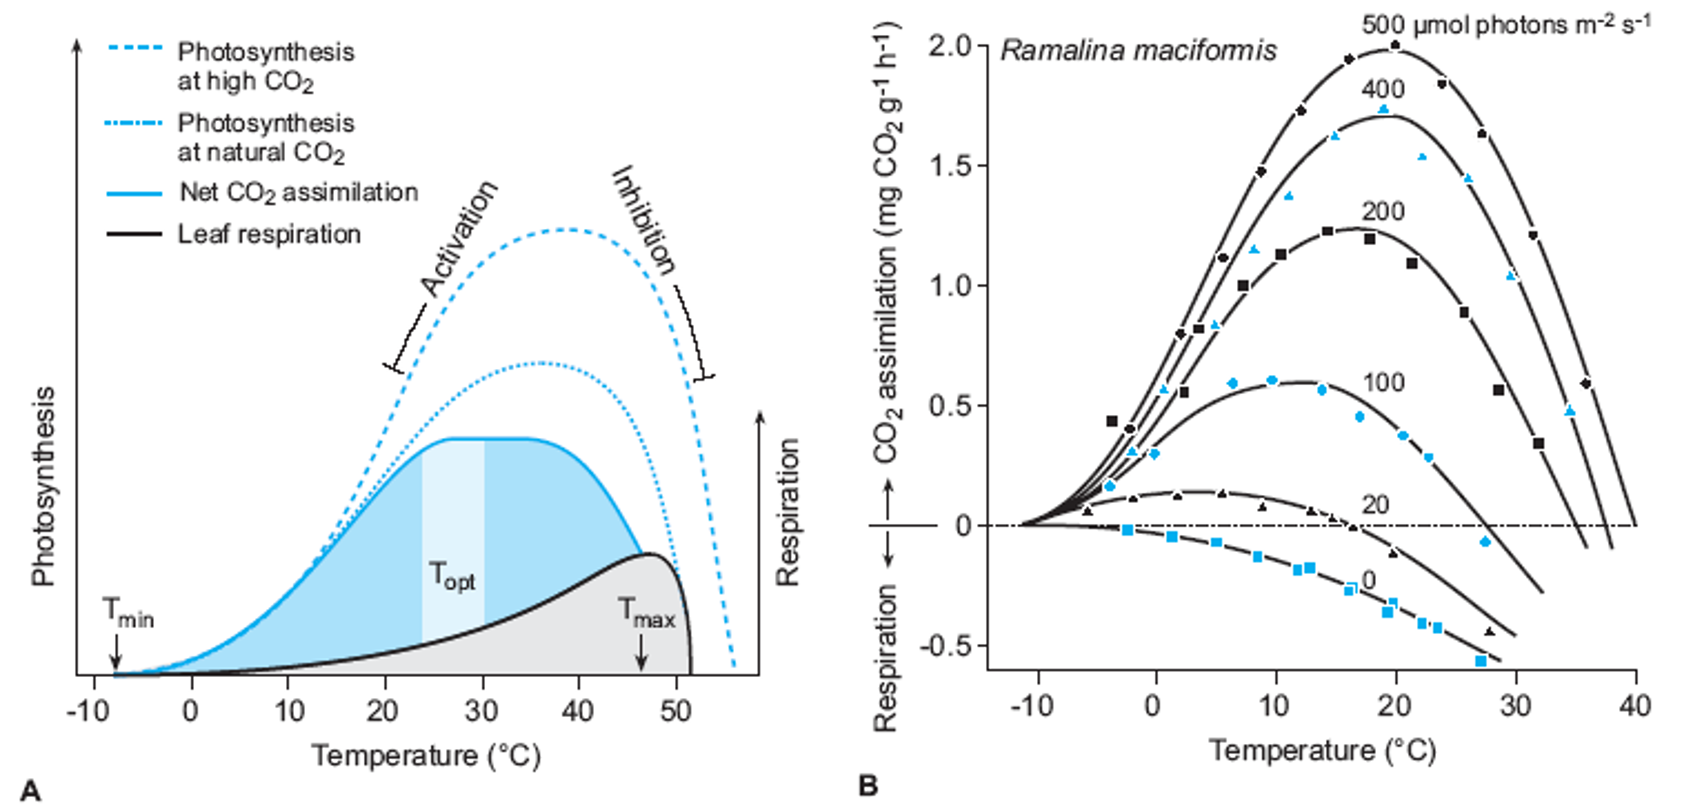
\includegraphics[width=0.8\linewidth]{figures/chap2/Trespons_interactions} 

}

\caption{Temperature responses of photosynthesis, respiration and net CO2 exchange, interaction with CO2 concentration (A) and light  (B)  Schulze ()}\label{fig:f23}
\end{figure}

\subsection{C3 photosynthesis}\label{c3-photosynthesis}

\subsubsection{Light response curve
models}\label{light-response-curve-models}

\begin{figure}

{\centering 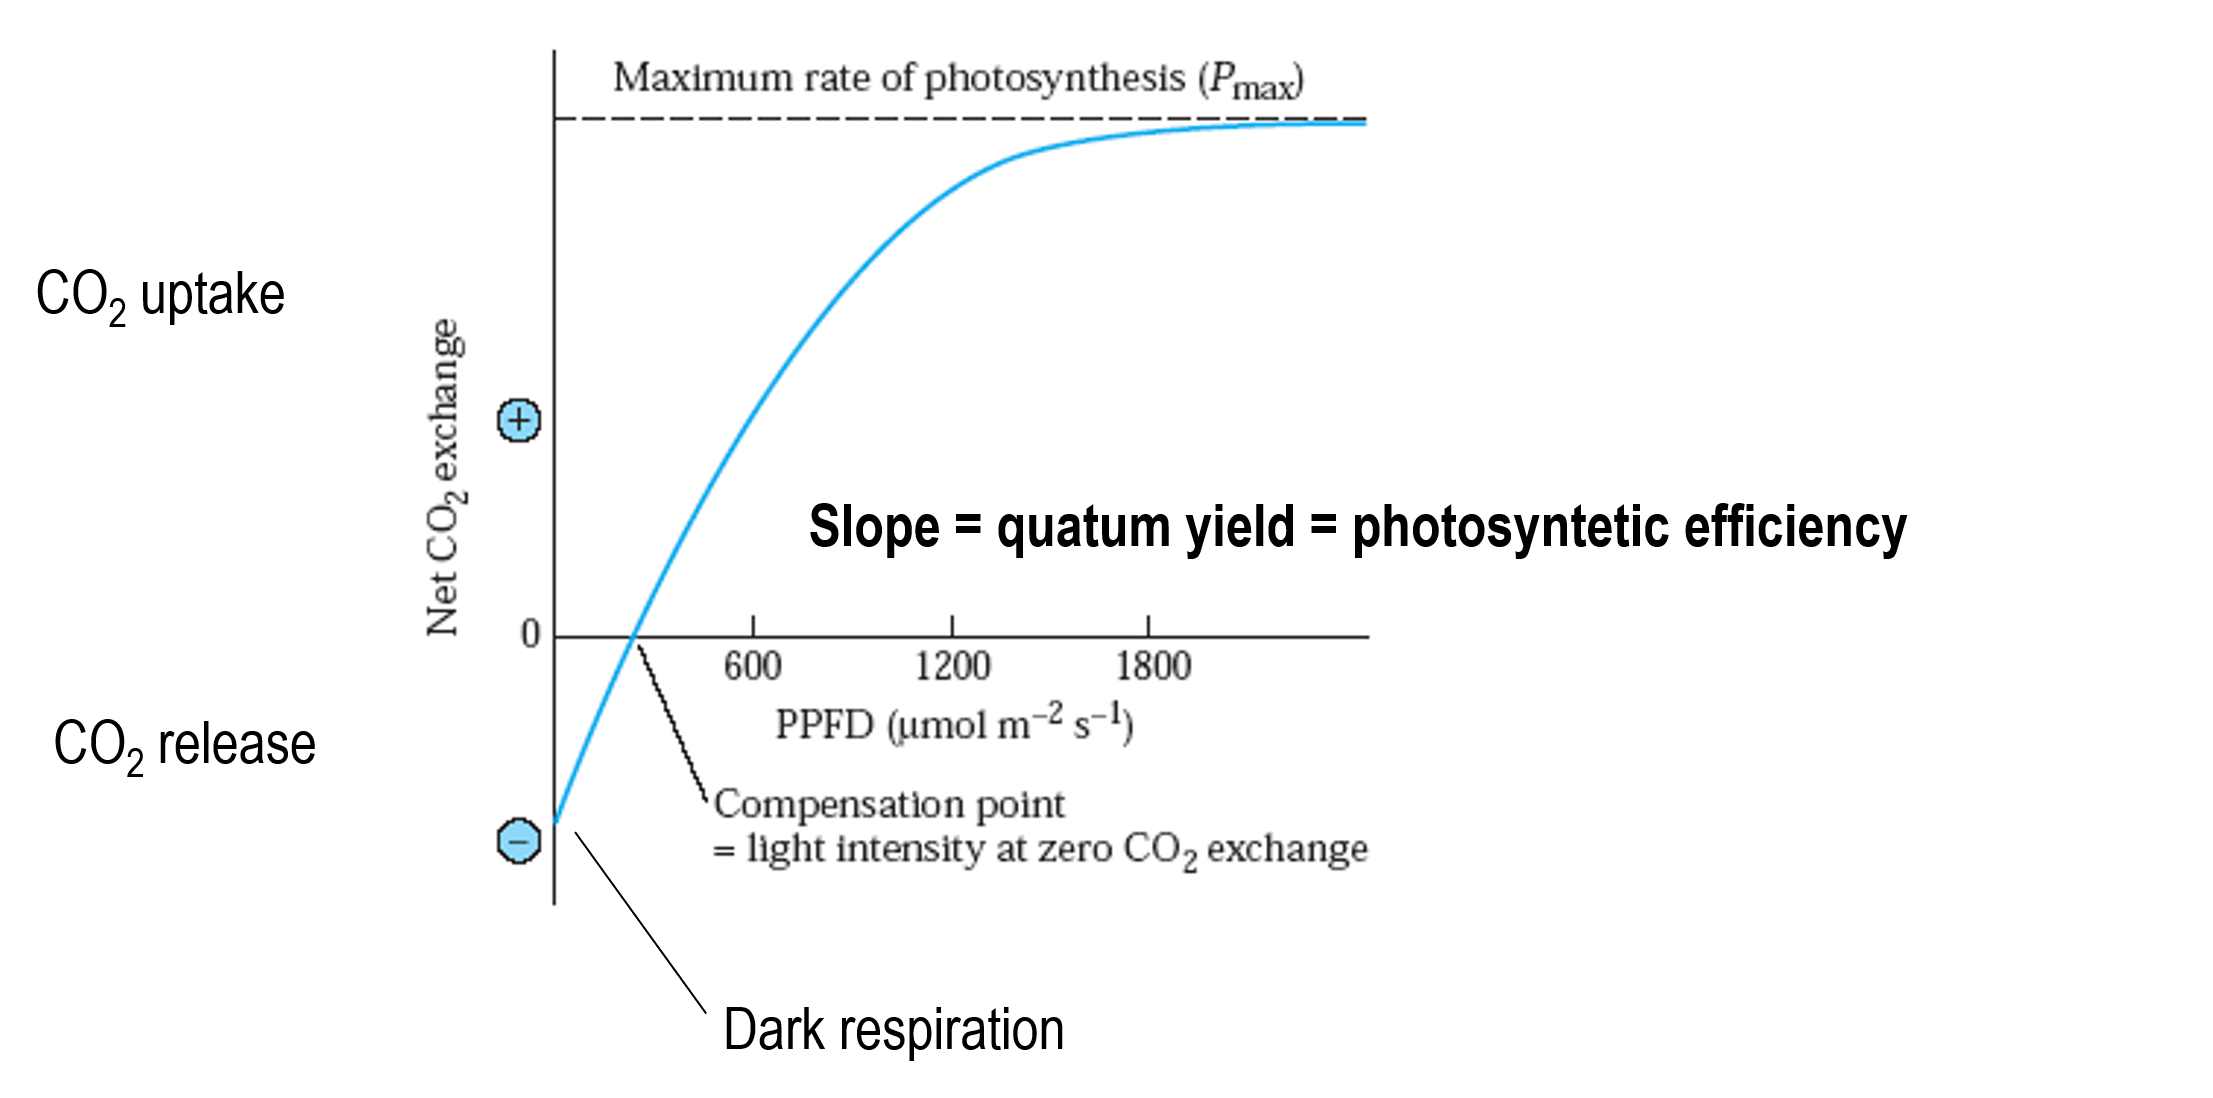
\includegraphics[width=0.8\linewidth]{figures/chap2/LRC} 

}

\caption{Conceptual figure of a leaf-level light reponse curve}\label{fig:f24}
\end{figure}

\begin{figure}

{\centering 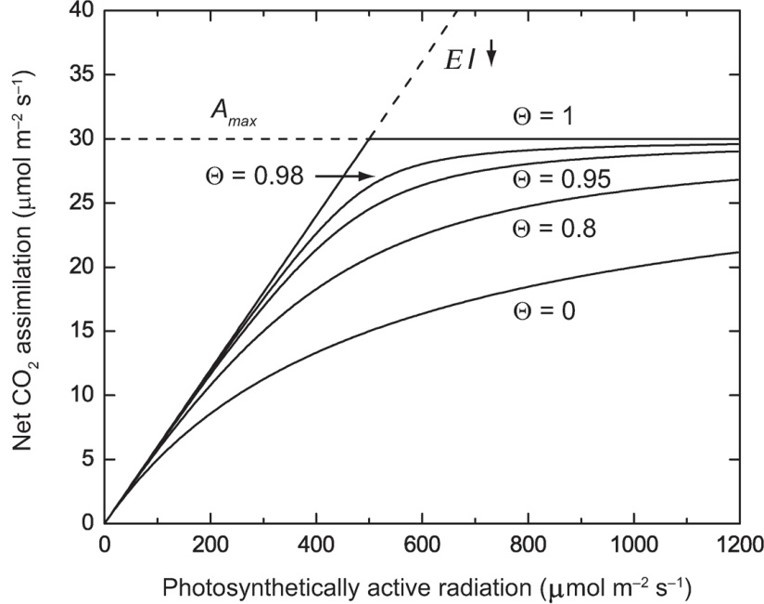
\includegraphics[width=0.8\linewidth]{figures/chap2/hyperbola} 

}

\caption{Co-limitation illustrated for photosynthetic response to light. The two dashed lines show the rates Amax adn EI The solid lines show the co-limited rate. (Bonan 2019)}\label{fig:f25}
\end{figure}

\subsubsection{Light use efficiency
models}\label{light-use-efficiency-models}

\begin{figure}

{\centering 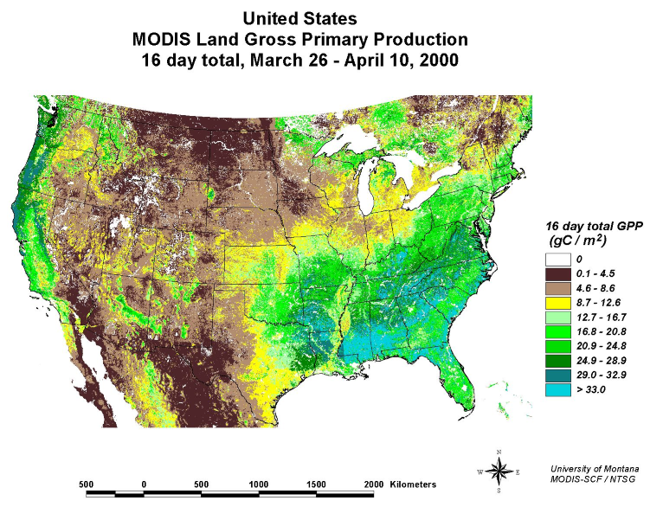
\includegraphics[width=0.8\linewidth]{figures/chap2/MODIS_GPP} 

}

\caption{MODIS based GPP map of the US, based on a LUE model.}\label{fig:f26}
\end{figure}

\subsubsection{The Farquahar model}\label{the-farquahar-model}

\begin{figure}

{\centering 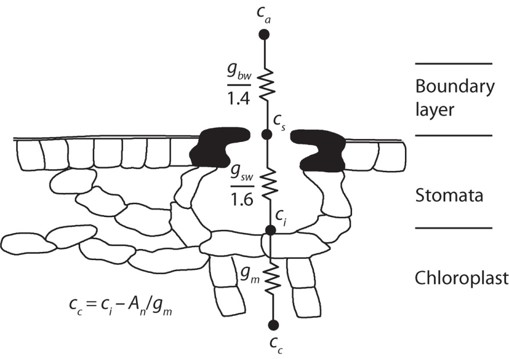
\includegraphics[width=0.8\linewidth]{figures/chap2/conductance} 

}

\caption{Diffusion of CO2 from free air across the leaf boundary layer and through stomata to the intercellular space. Diffusion to the chloroplast is additionally regulated by mesophyl conductance. (Bonan 2019)}\label{fig:f27}
\end{figure}

\begin{figure}

{\centering 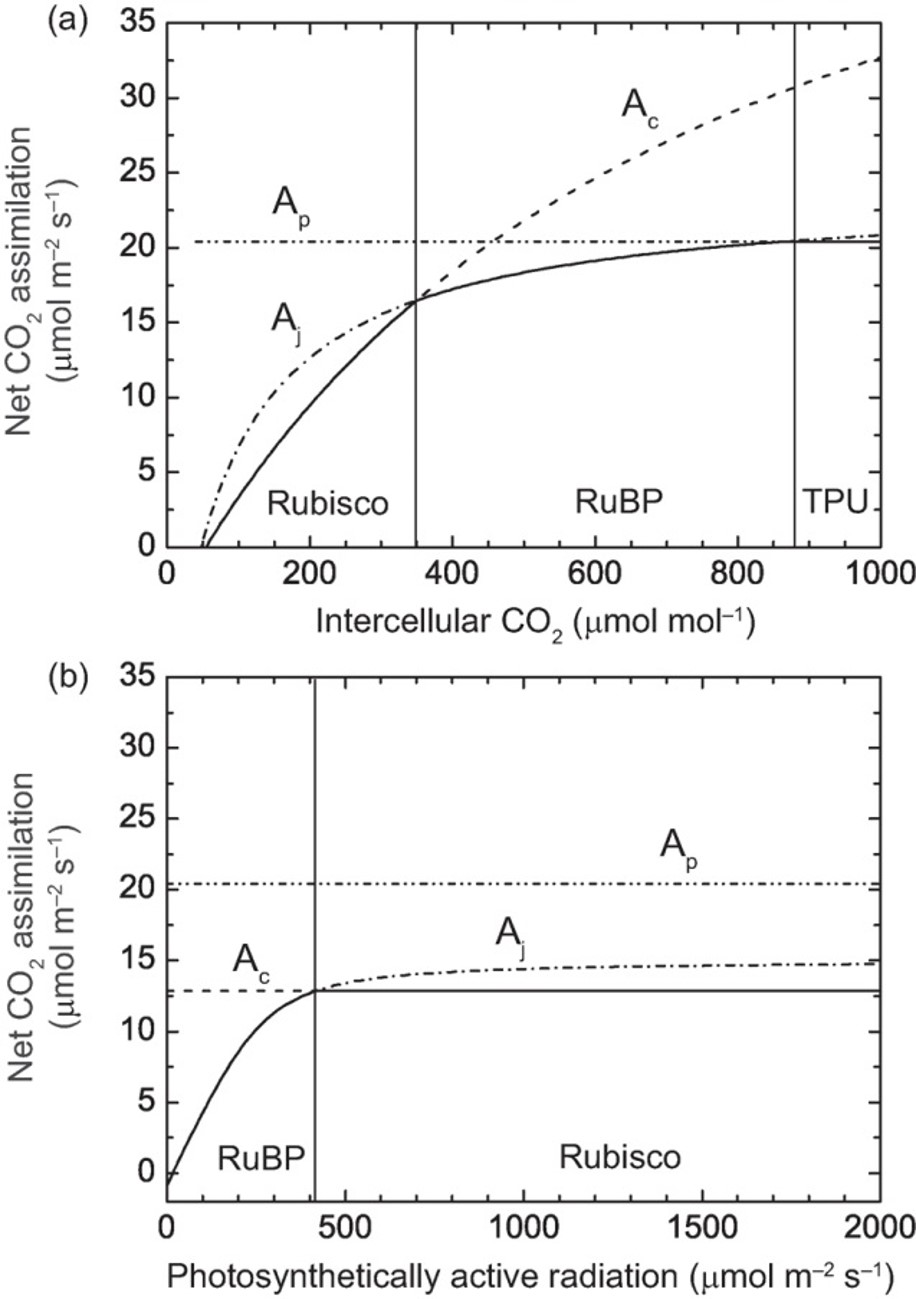
\includegraphics[width=0.8\linewidth]{figures/chap2/simulated_responses} 

}

\caption{Simulated responses of C3 photosynthesis in relation to (a) intercellular CO2 (at I↓ = 2000 μmol m–2 s–1) and (b) photosynthetically active radiation (at ci = 266 μmol mol–1). (Bonan 2019)}\label{fig:f28}
\end{figure}

\begin{itemize}
\tightlist
\item
  UCL 4.6.1
\item
  Bonan, Chapter 11.1 The FvCB model Most equations between 11.1 and
  11.31 Figure 11.2 a and b Table 11.1 for parameters values + a few
  simulations to illustrate Table 11.4
\end{itemize}

\subsection{Parameter and temperature
dependencies}\label{parameter-and-temperature-dependencies}

\begin{figure}

{\centering 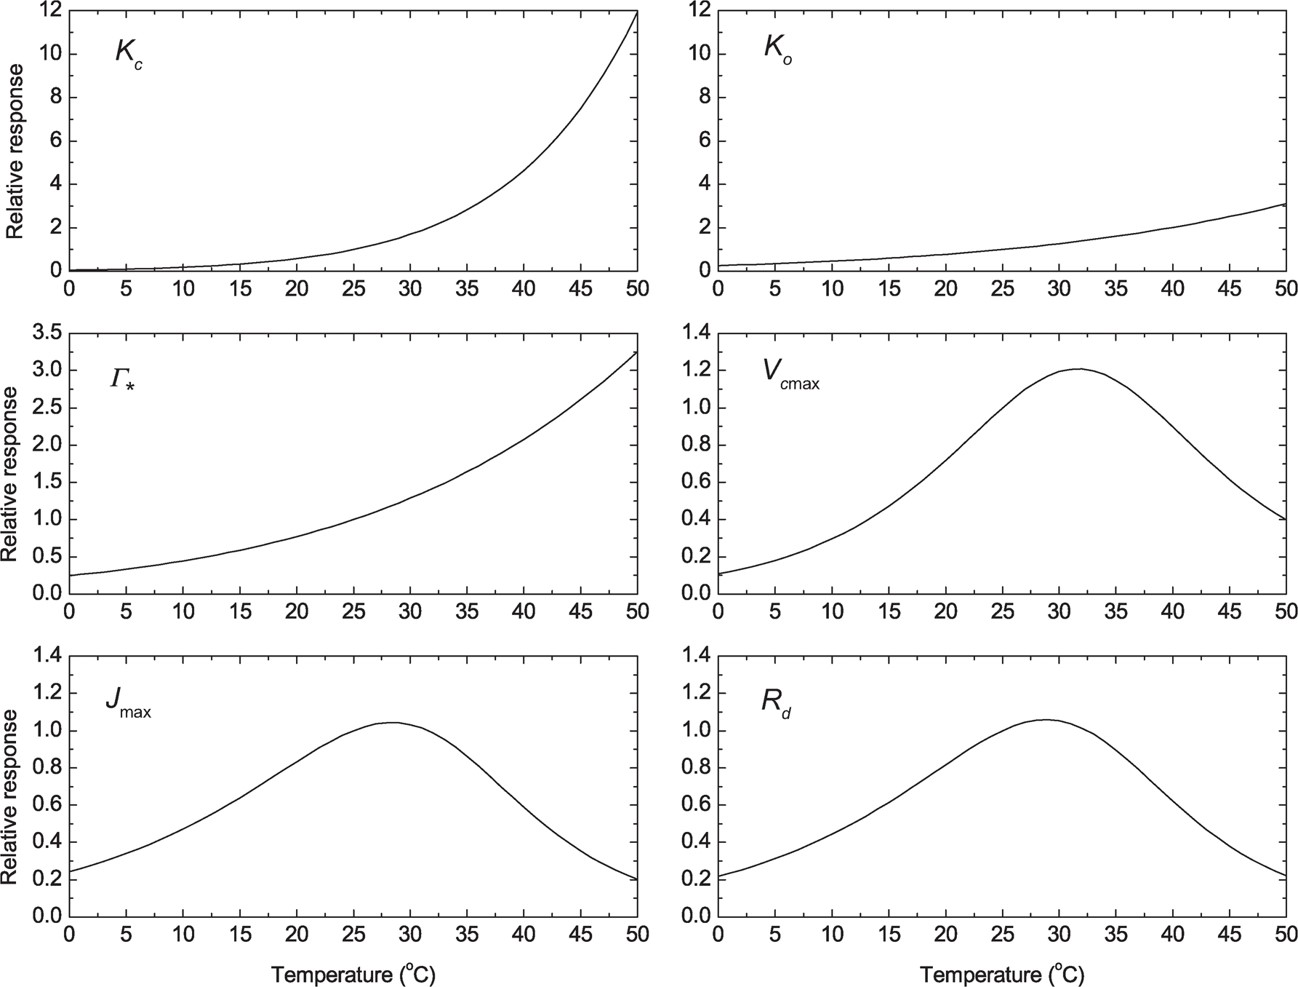
\includegraphics[width=0.8\linewidth]{figures/chap2/temp_responses} 

}

\caption{Relative temperature responses of the parameters of the Farquhar model (Bonan 2019)}\label{fig:f28bis}
\end{figure}

\begin{figure}

{\centering 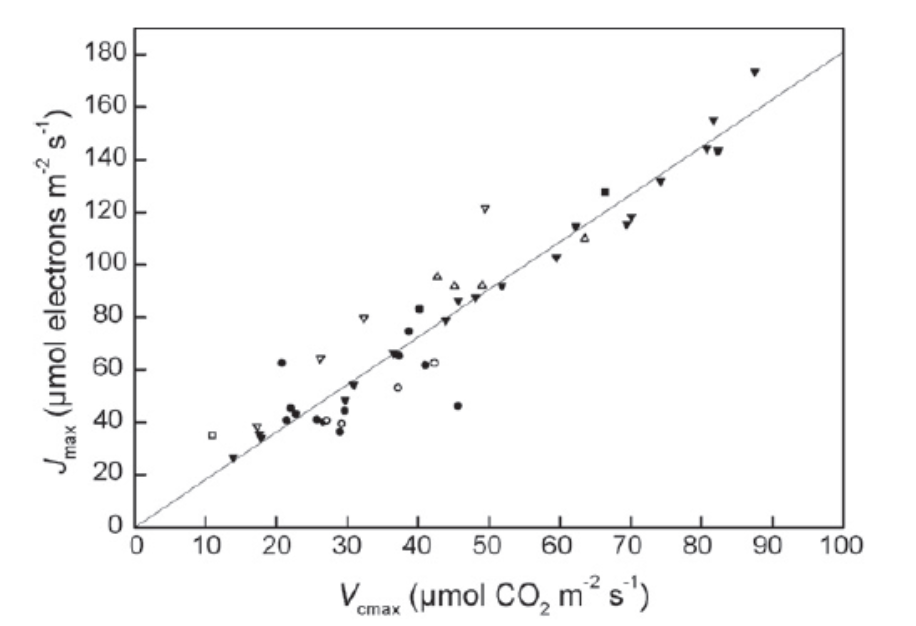
\includegraphics[width=0.8\linewidth]{figures/chap2/vcmax_jmax} 

}

\caption{Linear relation between observed Vcmax and Jmax values for Beech (Verbeeck et al. 2008)}\label{fig:f29}
\end{figure}

\begin{figure}

{\centering 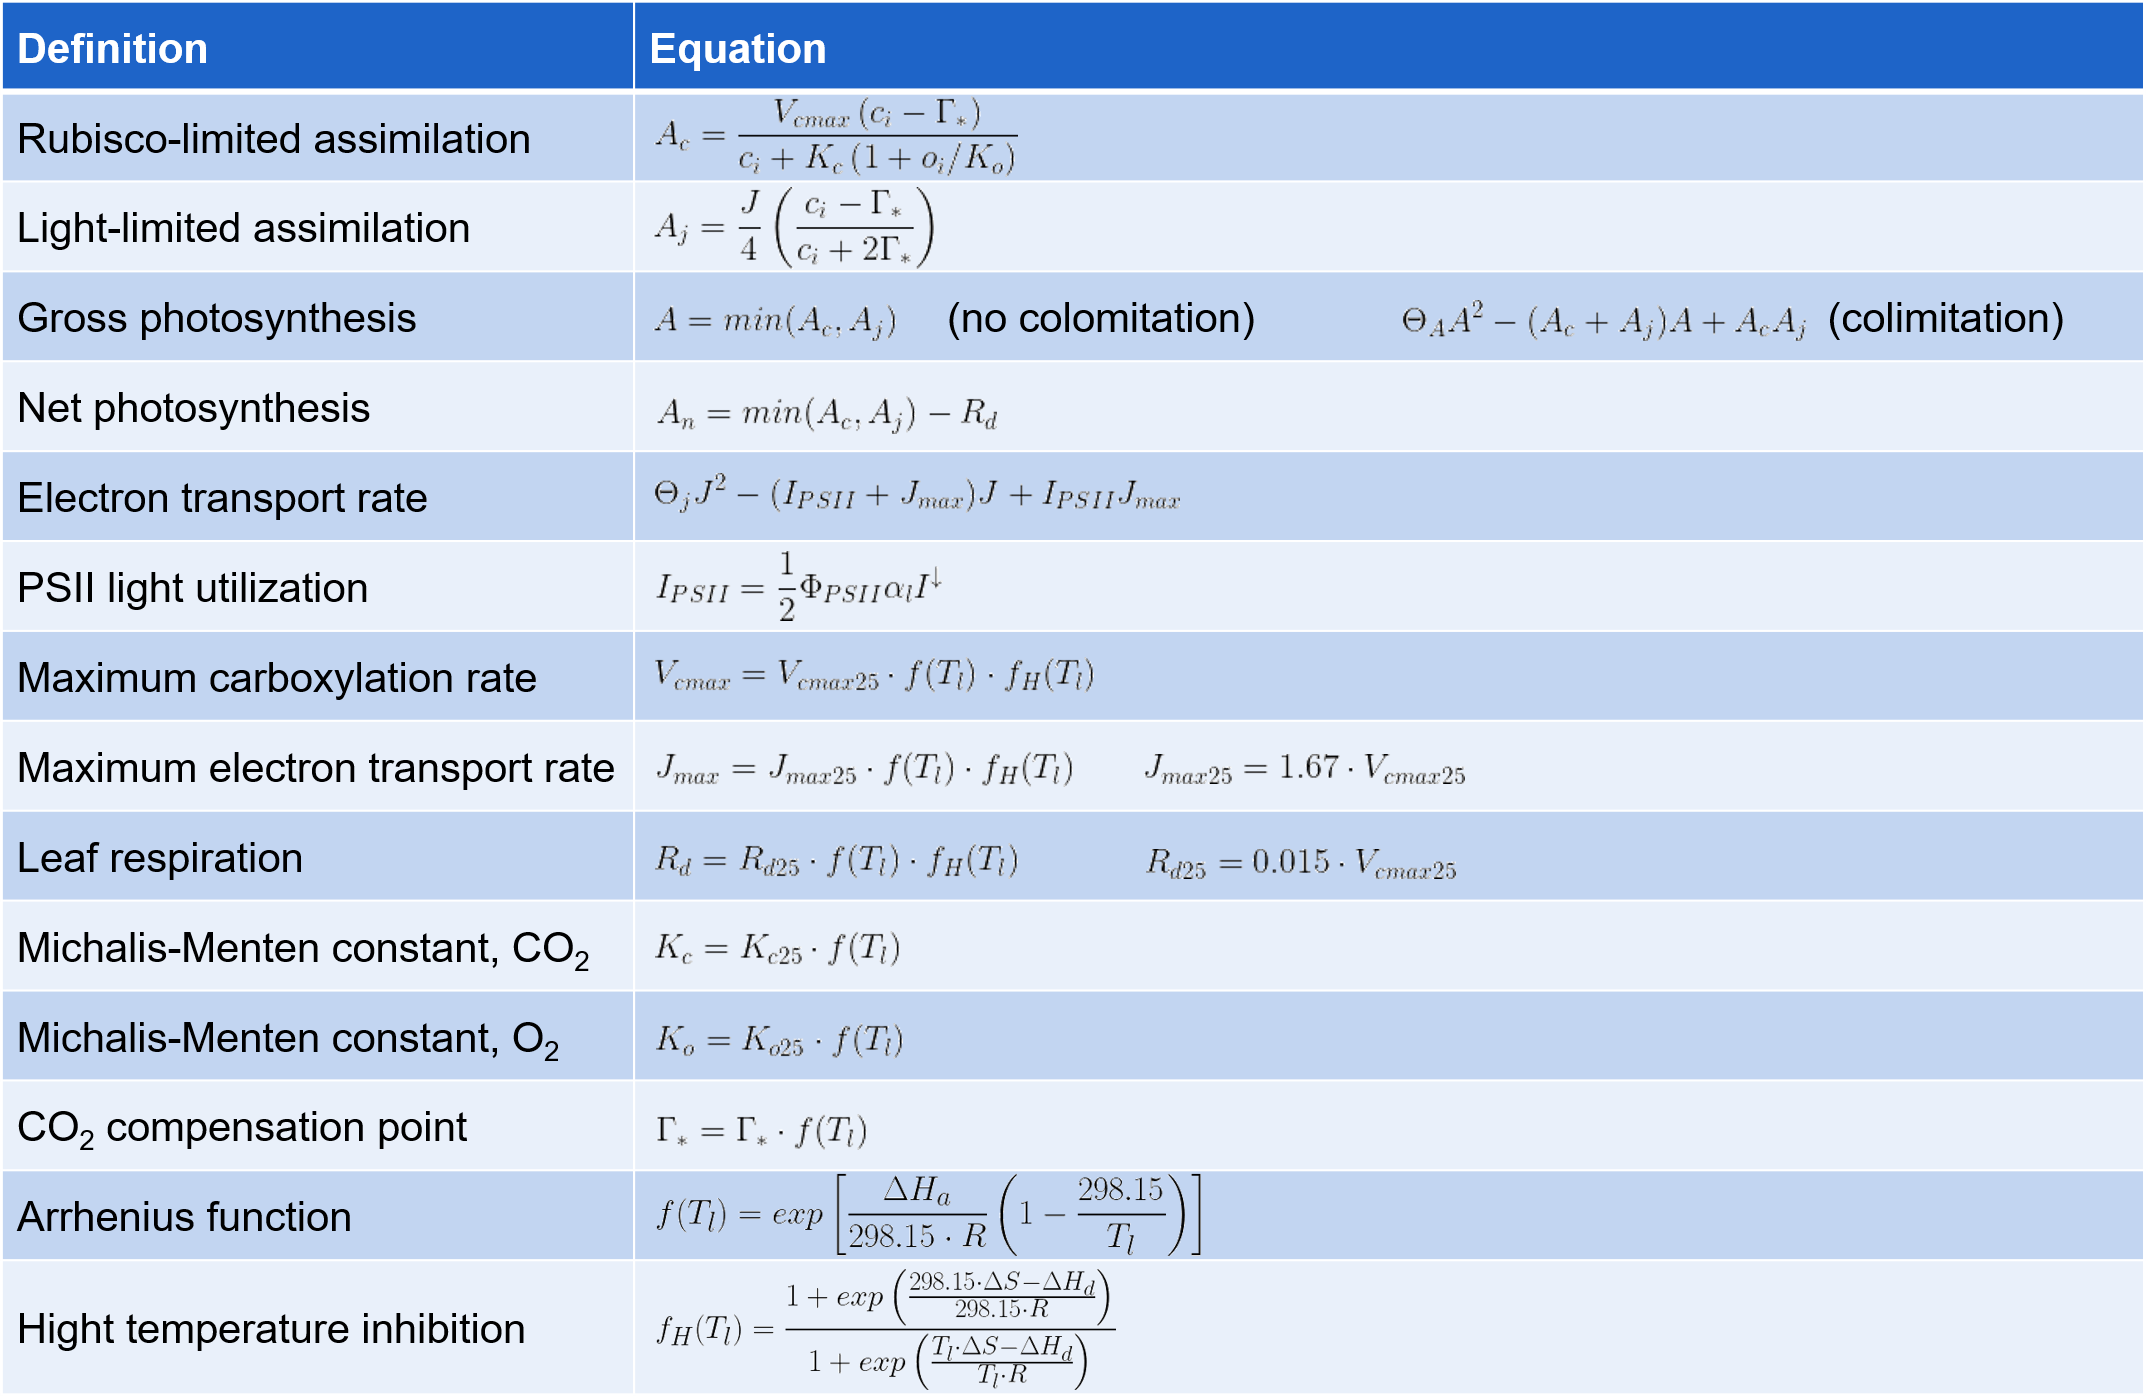
\includegraphics[width=0.8\linewidth]{figures/chap2/full_farquhar} 

}

\caption{Equations of the full Farquhar model}\label{fig:f210}
\end{figure}

\begin{itemize}
\tightlist
\item
  Bonan, Chapter 11.2 Equations 11.34-11.37 Table 11.2 Figure 11.3 for
  illustration
\end{itemize}

Summary with Table 11.5 and Figure 11.4

\subsection{C4 photosynthesis}\label{c4-photosynthesis}

\begin{itemize}
\tightlist
\item
  Bonan, Chapter 11.7 PEP carboxylase Equations 11.69-11.74 Find an
  illustration
\end{itemize}

\begin{figure}

{\centering 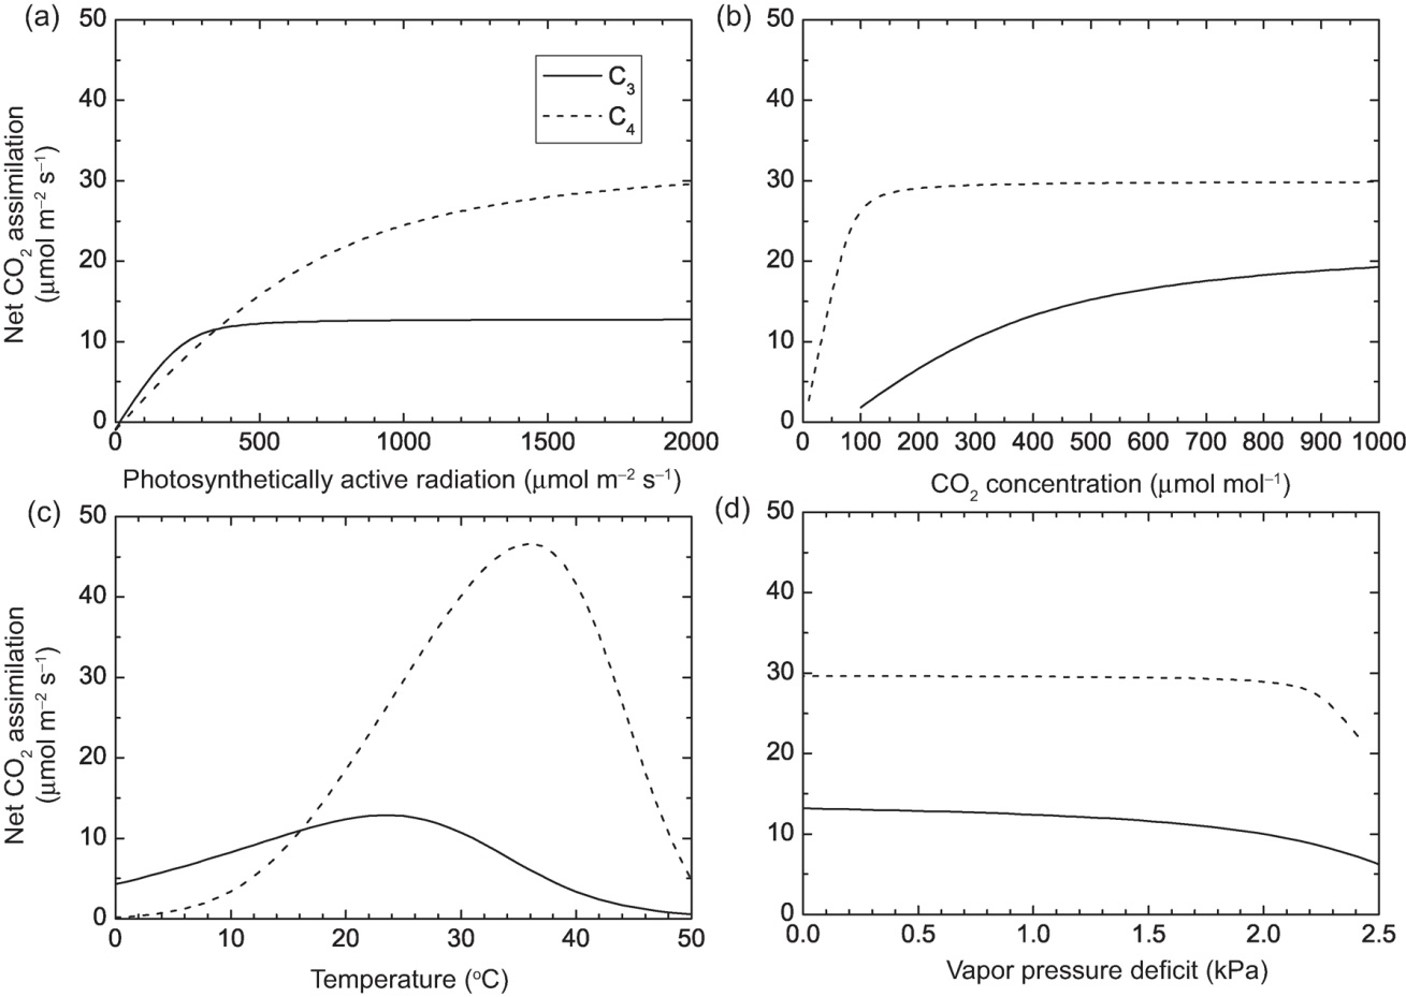
\includegraphics[width=0.8\linewidth]{figures/chap2/c3_c4} 

}

\caption{Comparison of C3 and C4 photosynthesis in response to (a) photosynthetically active radiation, (b) ambient CO2 concentration, (c) leaf temperature, and (d) vapor pressure deficit. In this figure, stomatal conductance is calculated using the Ball–Berry model and ci is obtained from the diffusion equation}\label{fig:f210b}
\end{figure}

\section{Stomatal models}\label{stomatal-models}

\subsection{Refreshing the basic
knowledge}\label{refreshing-the-basic-knowledge-1}

\begin{figure}

{\centering 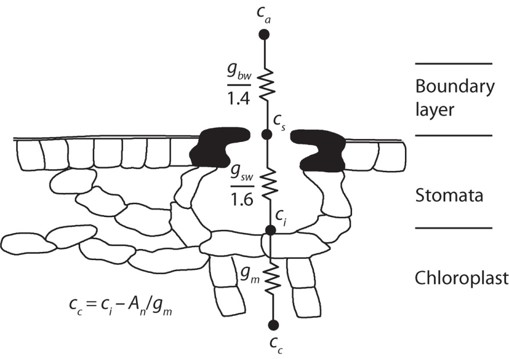
\includegraphics[width=0.8\linewidth]{figures/chap2/conductance} 

}

\caption{Diffusion of CO2 from free air across the leaf boundary layer and through stomata to the intercellular space. Diffusion to the chloroplast is additionally regulated by mesophyl conductance. (Bonan 2019)}\label{fig:f211}
\end{figure}

\begin{figure}

{\centering 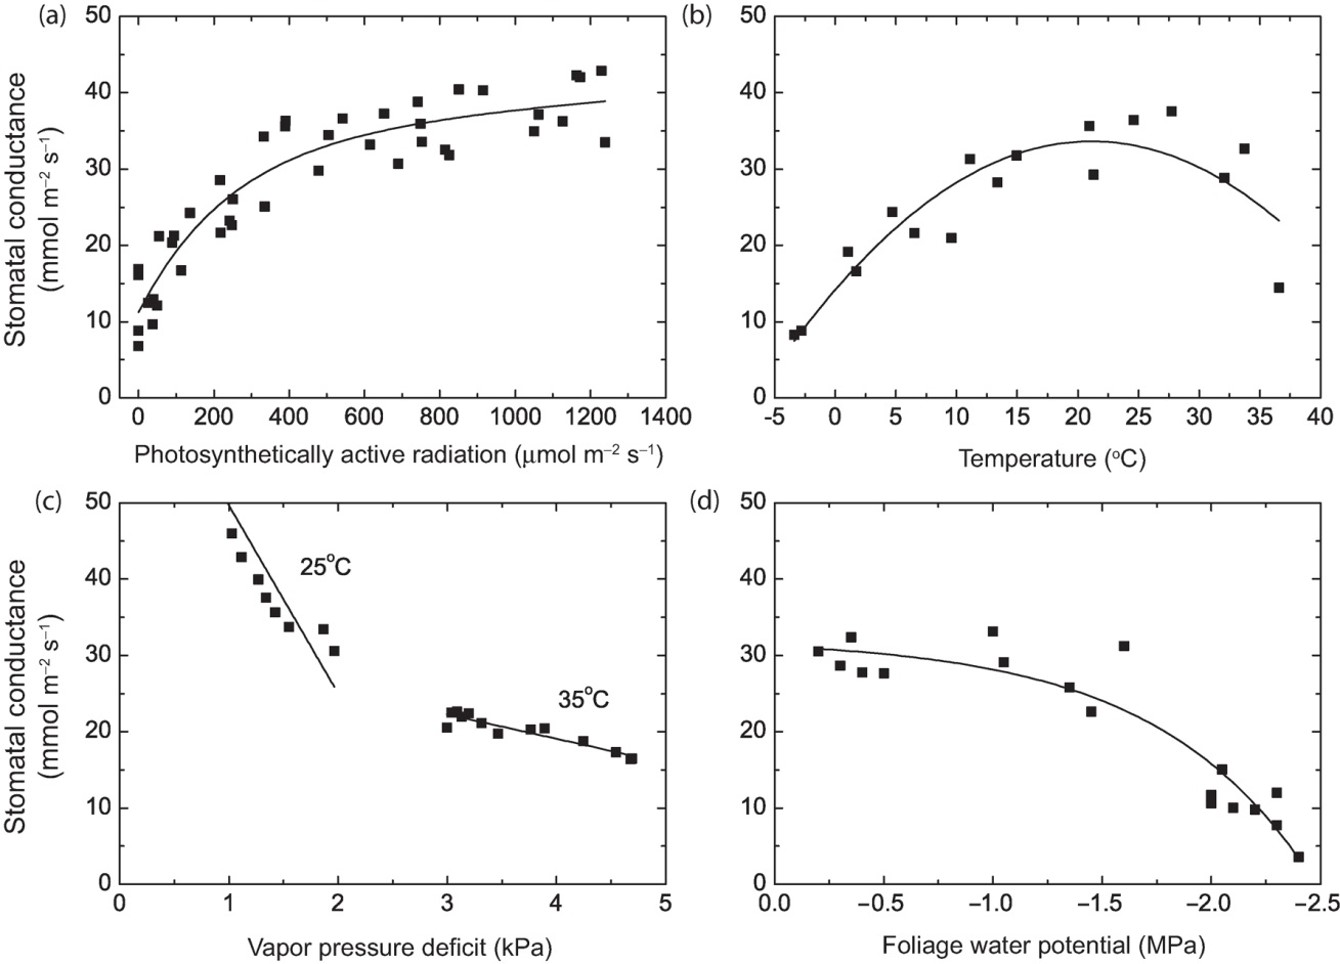
\includegraphics[width=0.8\linewidth]{figures/chap2/gs_obs} 

}

\caption{Observed responses of stomatal conductance for Pinus banksiana. (Bonan 2019)}\label{fig:f212}
\end{figure}

\subsection{Empirical multiplicative
models}\label{empirical-multiplicative-models}

\begin{itemize}
\tightlist
\item
  Bonan, Chapter 12.2
\end{itemize}

\subsection{Semiempirical photosynthesis-based
models}\label{semiempirical-photosynthesis-based-models}

\begin{itemize}
\tightlist
\item
  Bonan, Chapter 12.3
\end{itemize}

\begin{figure}

{\centering 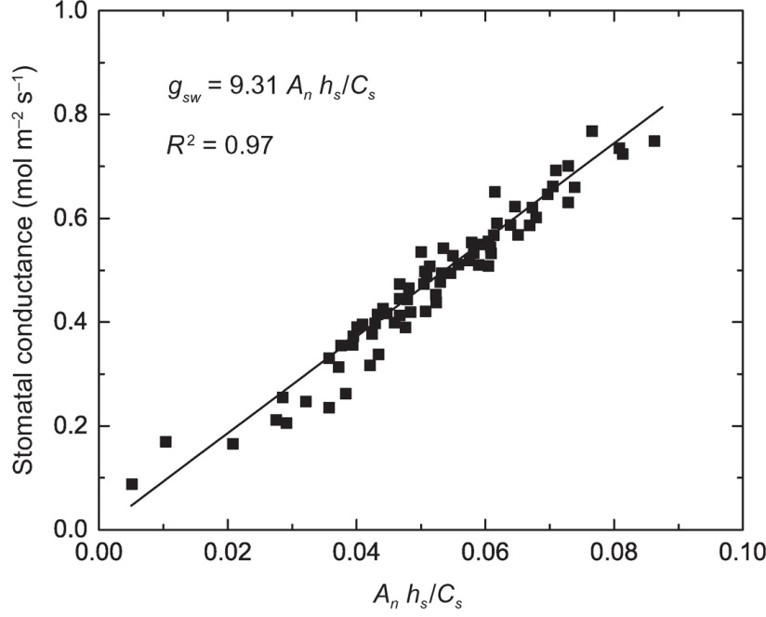
\includegraphics[width=0.8\linewidth]{figures/chap2/ball_berry} 

}

\caption{Relationship between stomatal conductance and Anhs/cs for soybean.(Bonan 2019)}\label{fig:f213}
\end{figure}

\begin{figure}

{\centering 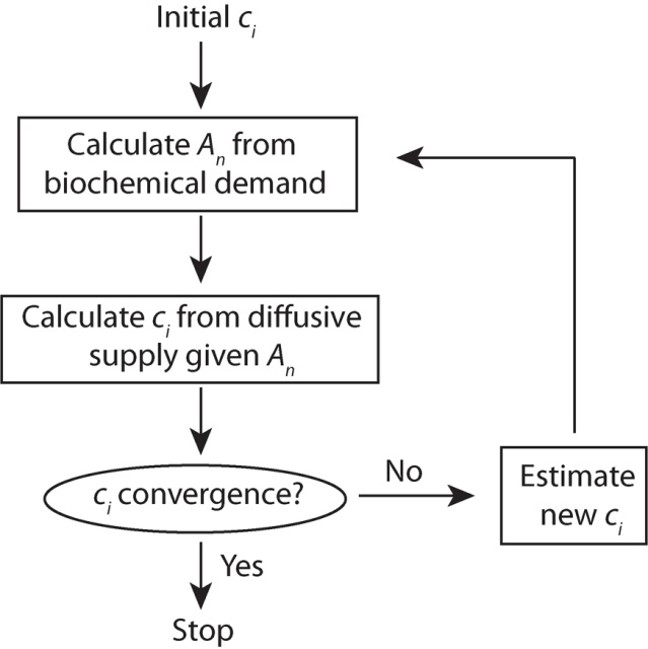
\includegraphics[width=0.8\linewidth]{figures/chap2/numerical_solution} 

}

\caption{Flow diagram of the iterative procedure to numerically calculate ci.(Bonan 2019)}\label{fig:f214}
\end{figure}

\subsection{WUE models and optimality
theory}\label{wue-models-and-optimality-theory}

\begin{itemize}
\tightlist
\item
  Bonan, Chapter 12.4 + add optimality approach from Prentice et al.
\end{itemize}

\begin{figure}

{\centering 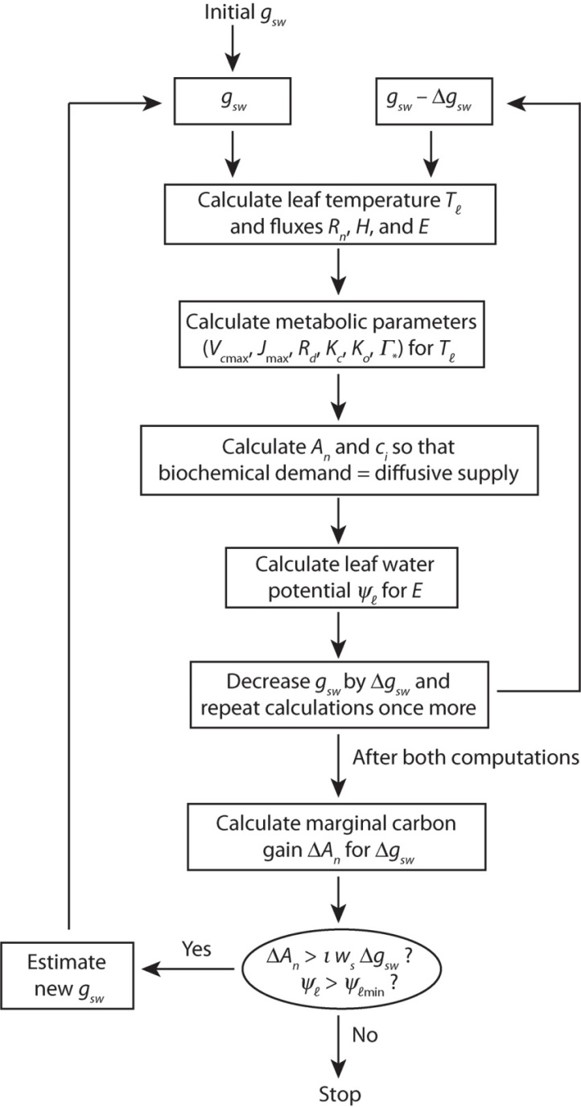
\includegraphics[width=0.8\linewidth]{figures/chap2/optimality} 

}

\caption{Flow diagram of leaf flux calculations to numerically solve for stomatal conductance that optimizes water-use efficiency.(Bonan 2019)}\label{fig:f215}
\end{figure}

\subsection{Soil drought stress}\label{soil-drought-stress}

\begin{figure}

{\centering 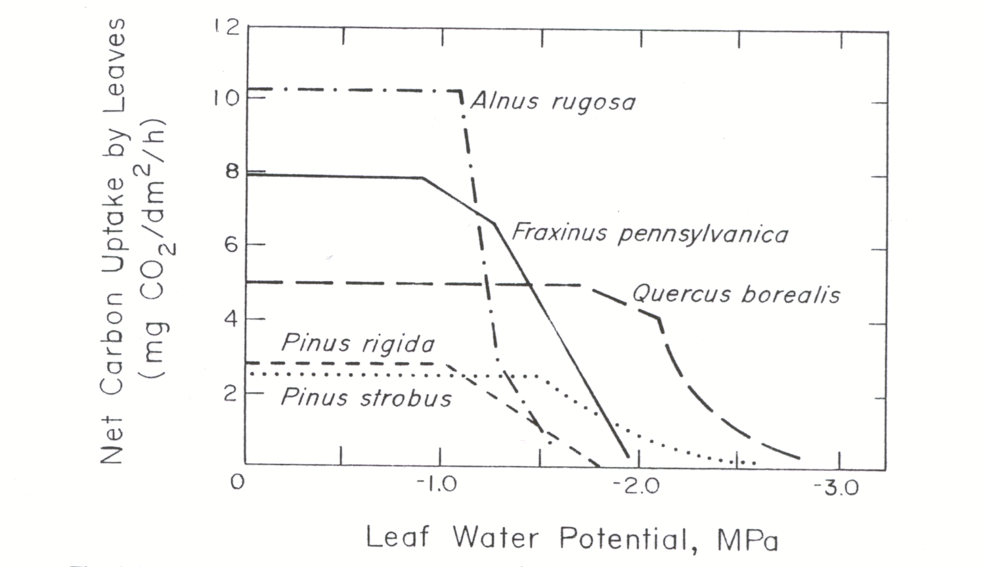
\includegraphics[width=0.8\linewidth]{figures/chap2/leafWP} 

}

\caption{Leaf carbon uptake in response to leaf water potential for multiple tree species.}\label{fig:f216}
\end{figure}

\begin{figure}

{\centering 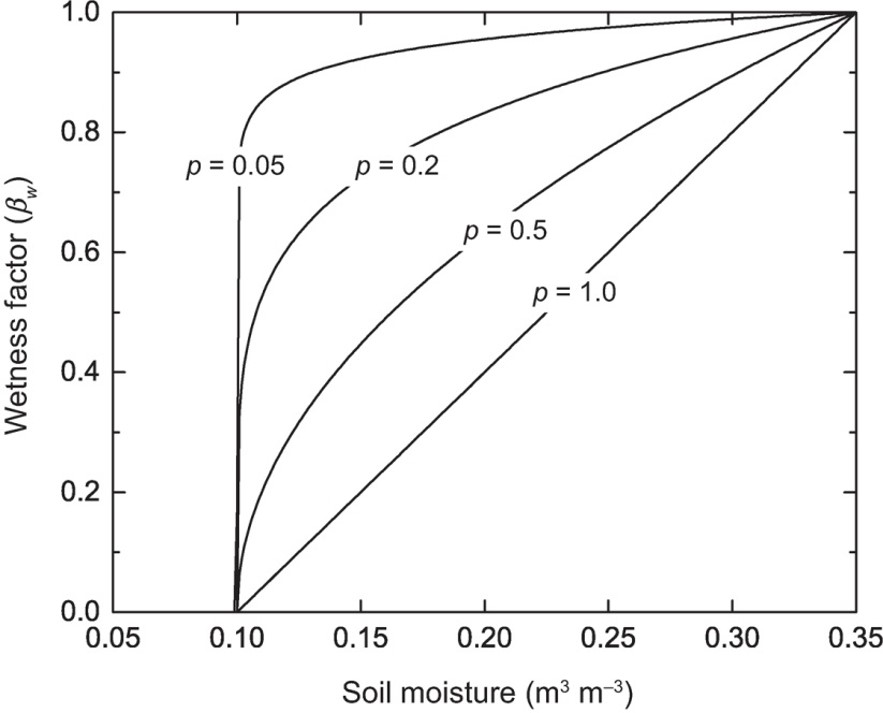
\includegraphics[width=0.8\linewidth]{figures/chap2/SWfactor} 

}

\caption{Soil moisture wetness factor in relation to volumetric water content. (Bonan 2019)}\label{fig:f217}
\end{figure}

\subsection{Hydraulic models}\label{hydraulic-models}

\begin{figure}

{\centering 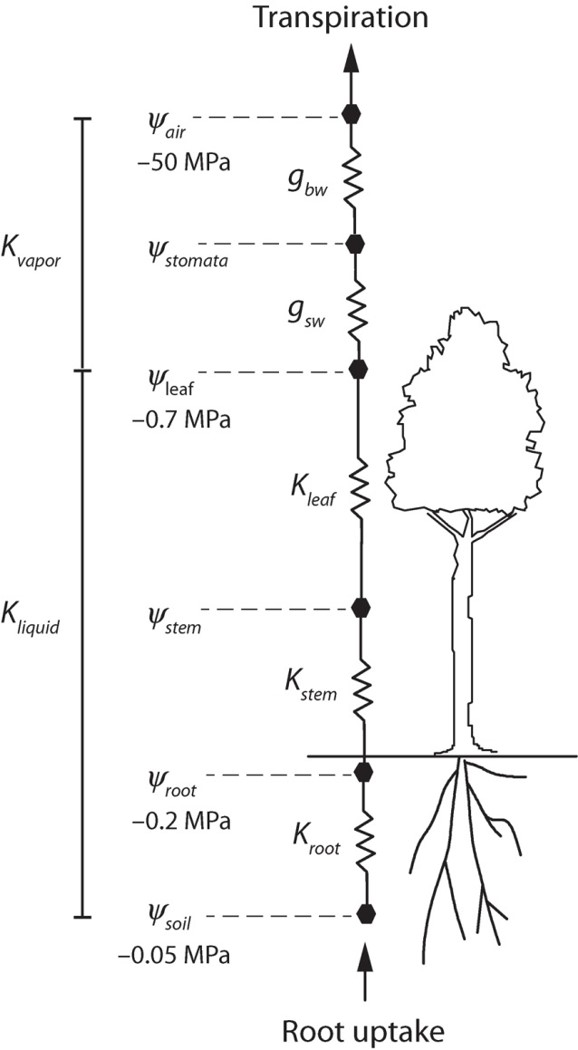
\includegraphics[width=0.8\linewidth]{figures/chap2/hydraulics} 

}

\caption{Flow of water and representative water potentials along the soil–plant–atmosphere continuum. Also shown are conductances along the hydraulic pathway.(Bonan 2019)}\label{fig:f218}
\end{figure}

\begin{figure}

{\centering 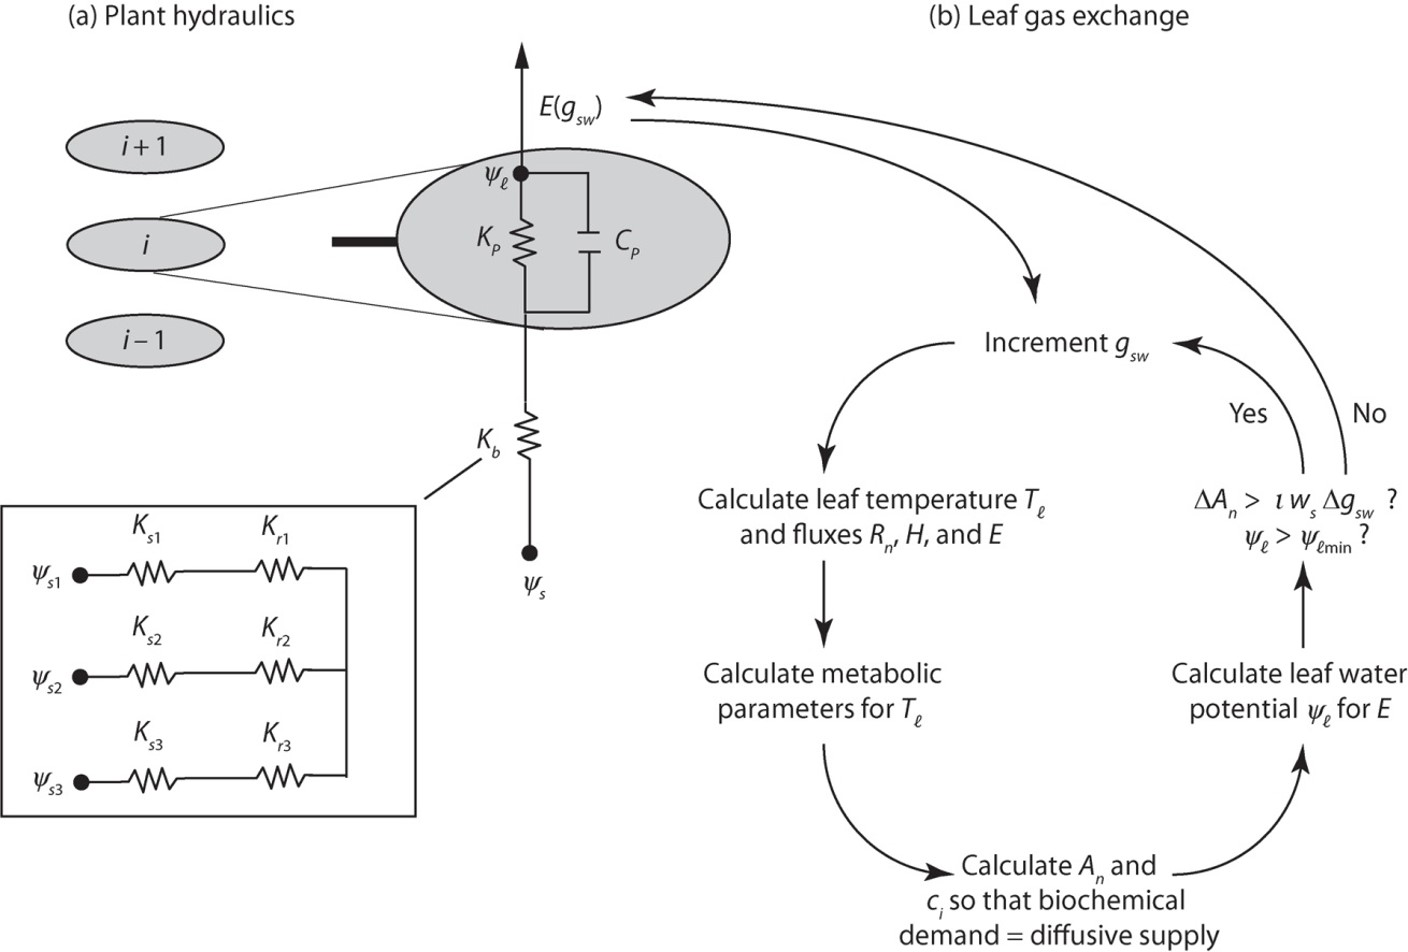
\includegraphics[width=0.8\linewidth]{figures/chap2/SPA} 

}

\caption{Depiction of (a) plant hydraulics and (b) leaf gas exchange in the Soil–Plant–Atmosphere (SPA) model. SPA is a multilayer canopy model.(Bonan 2019)}\label{fig:f219}
\end{figure}

\begin{figure}

{\centering 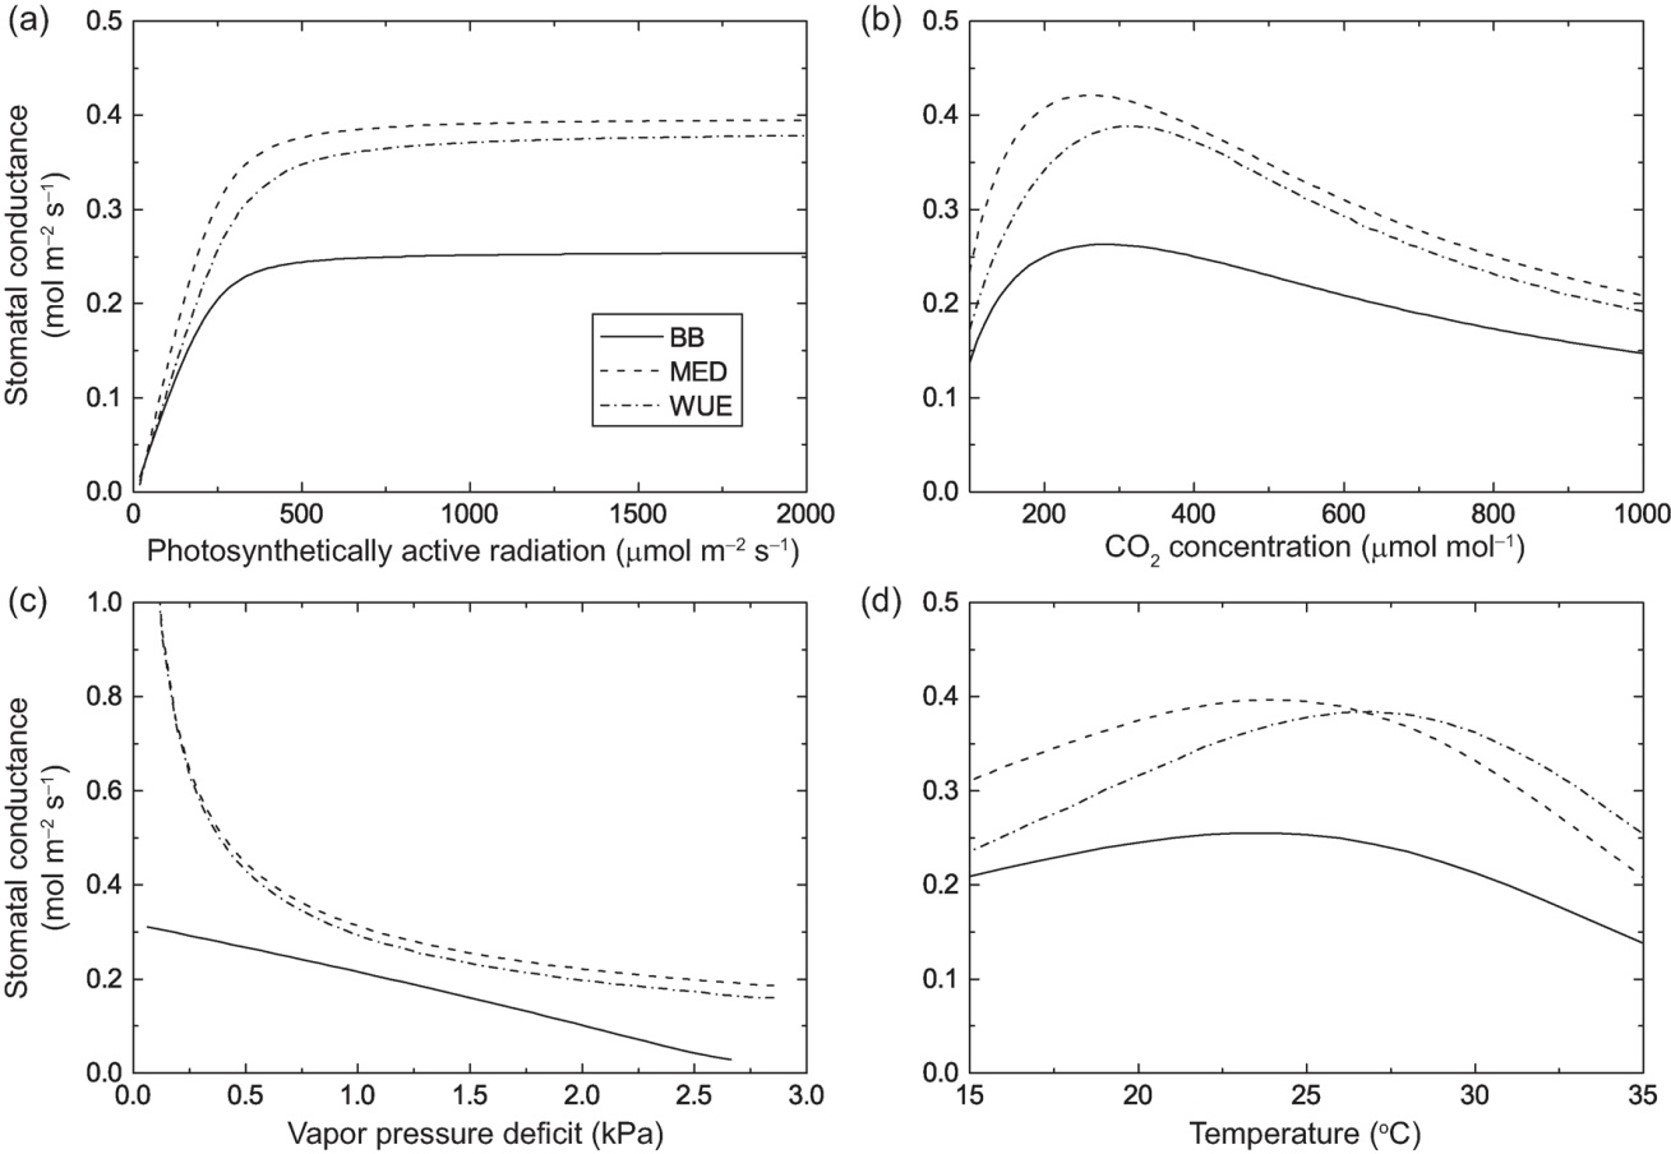
\includegraphics[width=0.8\linewidth]{figures/chap2/modelling_approaches} 

}

\caption{Simulated stomatal responses for various modelling approaches. (Bonan 2019)}\label{fig:f220}
\end{figure}

Figure 13.1 The soil-plant-atmosphere model Leaf water potential Plant
water uptake Resistance analogy Multinode models

\section{Upscaling from leaf to
canopy}\label{upscaling-from-leaf-to-canopy}

\begin{itemize}
\tightlist
\item
  Quickly introduce the problem of scaling in ecology (review paper of
  Jerome Chave) and refer to chapter 10 on upscalling
\item
  Canopy integration: LAI layers, etc\ldots{} Nice transition to chap 3
  with the interception of light by the canopy
\end{itemize}

Leaf microclimate and boundary layer processes in relation to leaf
dimension for sun and shade conditions.

\begin{figure}

{\centering 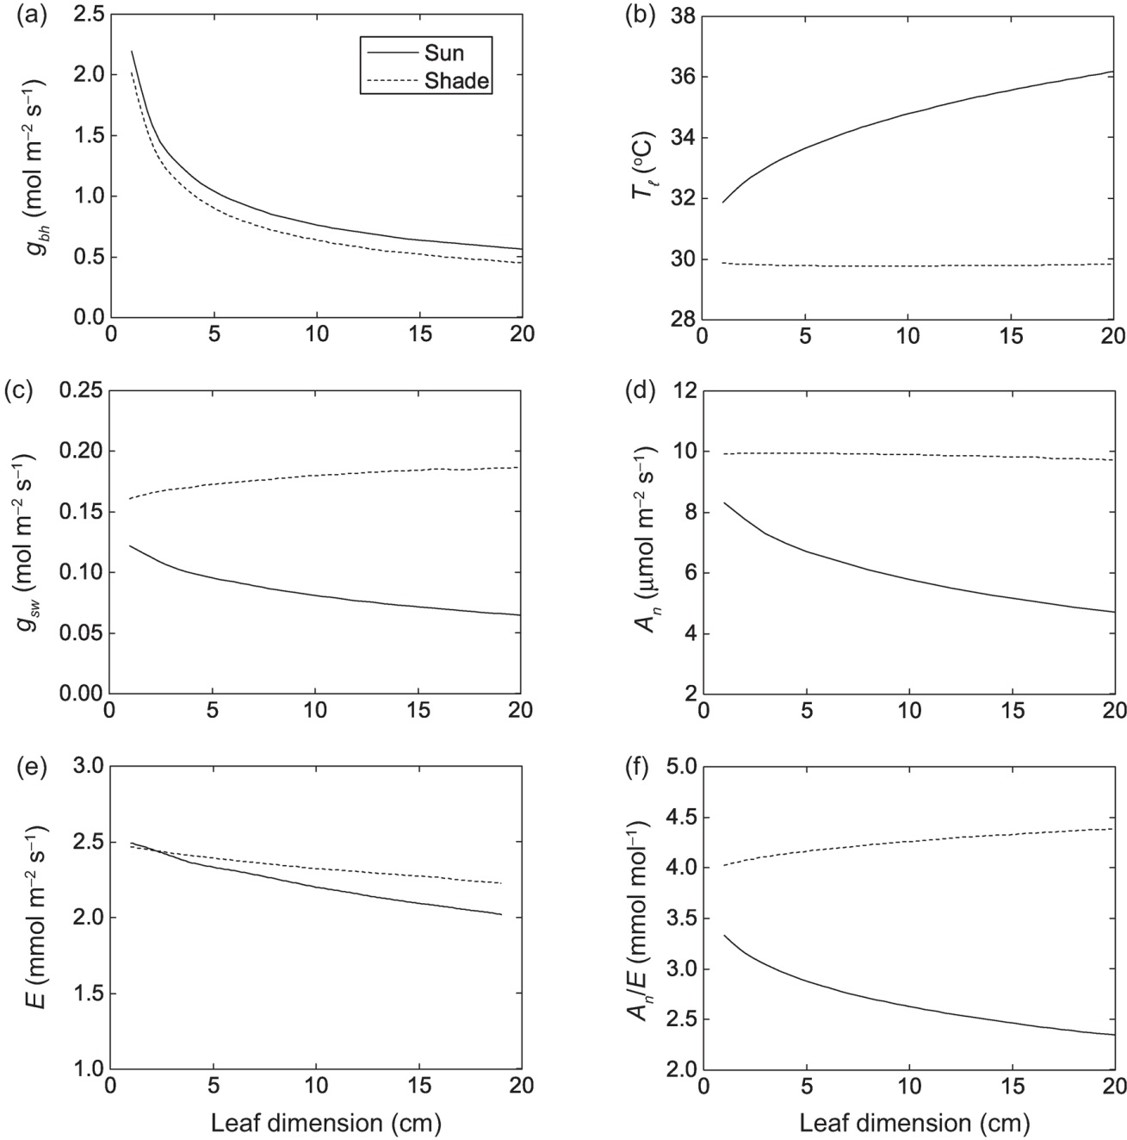
\includegraphics[width=0.8\linewidth]{figures/chap2/sun_shade} 

}

\caption{Leaf microclimate and boundary layer processes in relation to leaf dimension for sun and shade conditions.(Bonan 2019)}\label{fig:f221}
\end{figure}

\begin{figure}

{\centering 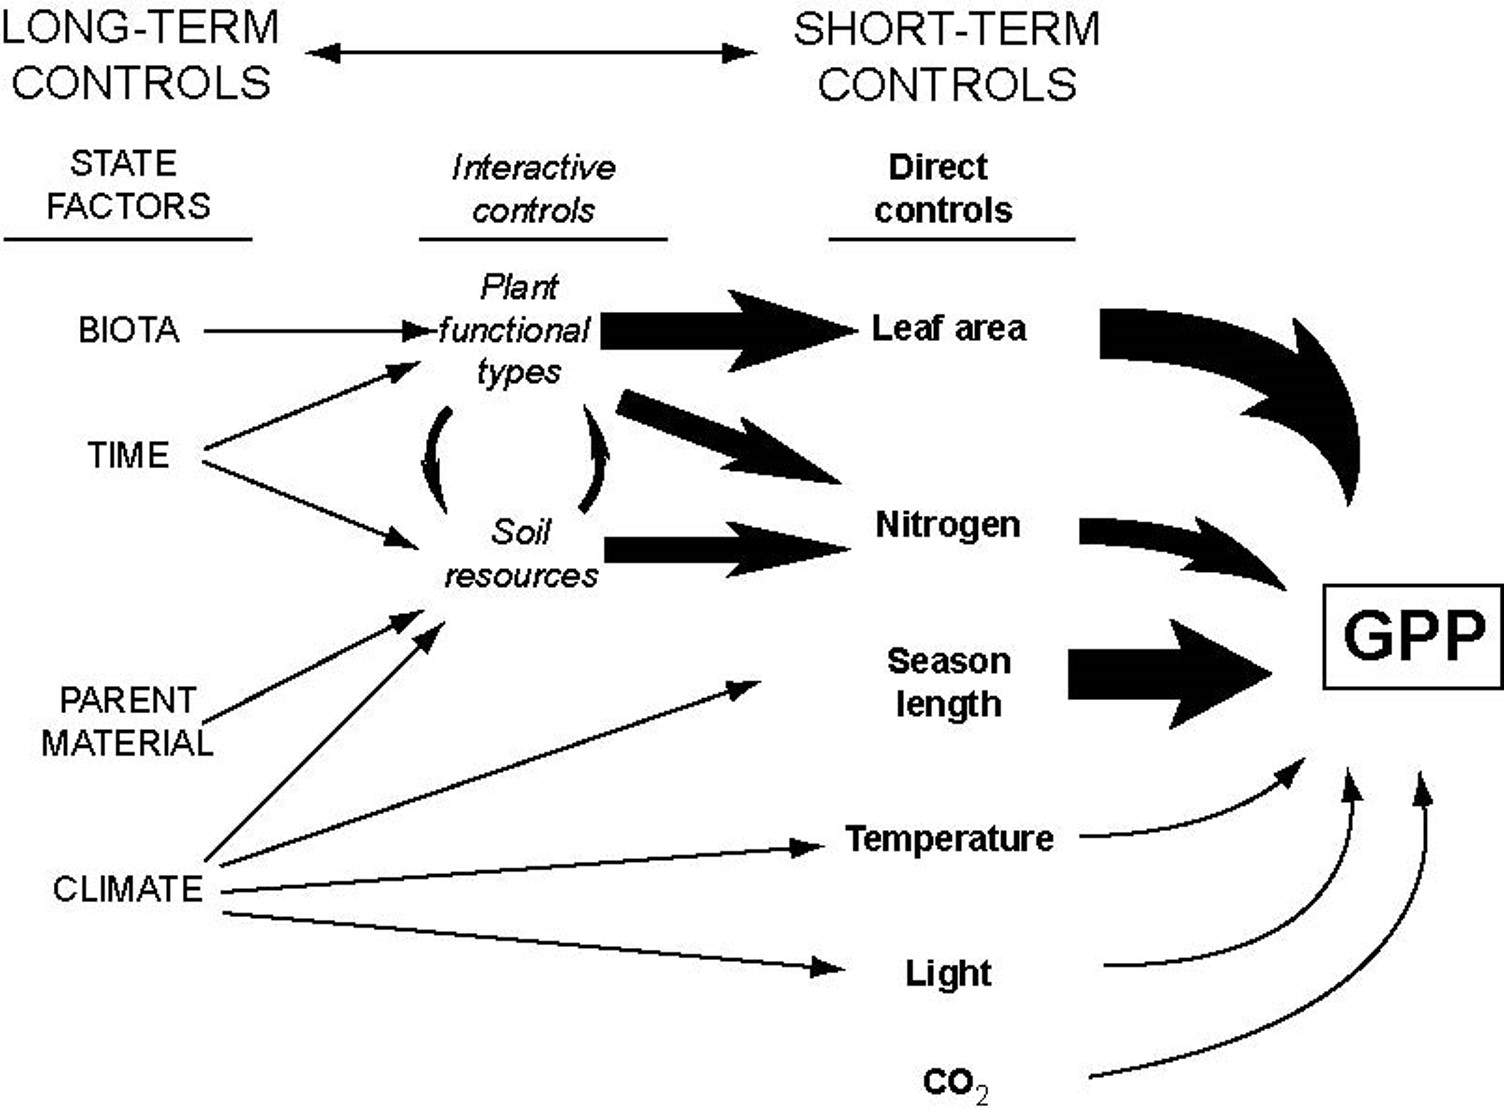
\includegraphics[width=0.8\linewidth]{figures/chap2/GPPcontrols} 

}

\caption{Controlling facors on ecosystem GPP. (Chapin)}\label{fig:f222}
\end{figure}

\section{Case studies}\label{case-studies}

\subsection{Case study 2.1 Ozone impact on global
GPP}\label{case-study-2.1-ozone-impact-on-global-gpp}

\begin{figure}

{\centering 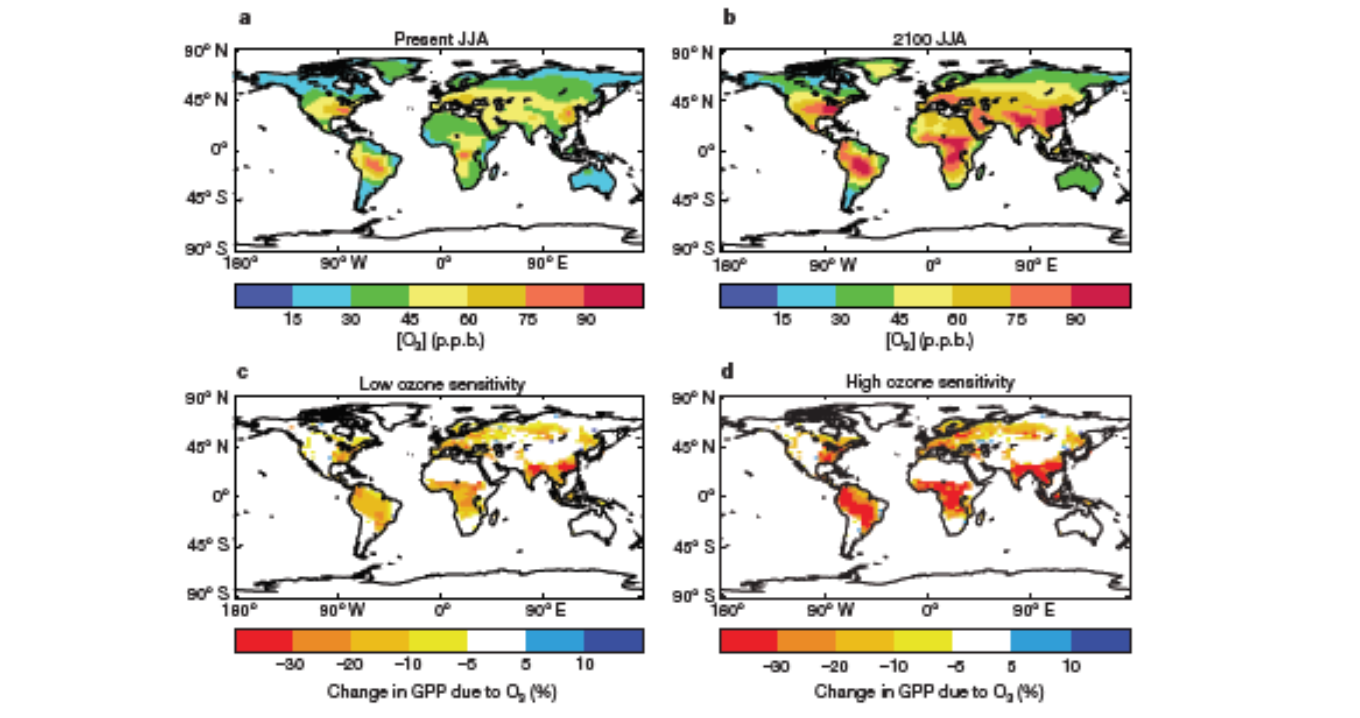
\includegraphics[width=0.8\linewidth]{figures/chap2/ozone} 

}

\caption{Simulated global GPP reduction in response to current and future atmospheric ozone concentrations}\label{fig:f223}
\end{figure}

\subsection{Case study 2.2 Drought impact on rainforest
GPP}\label{case-study-2.2-drought-impact-on-rainforest-gpp}

\begin{figure}

{\centering 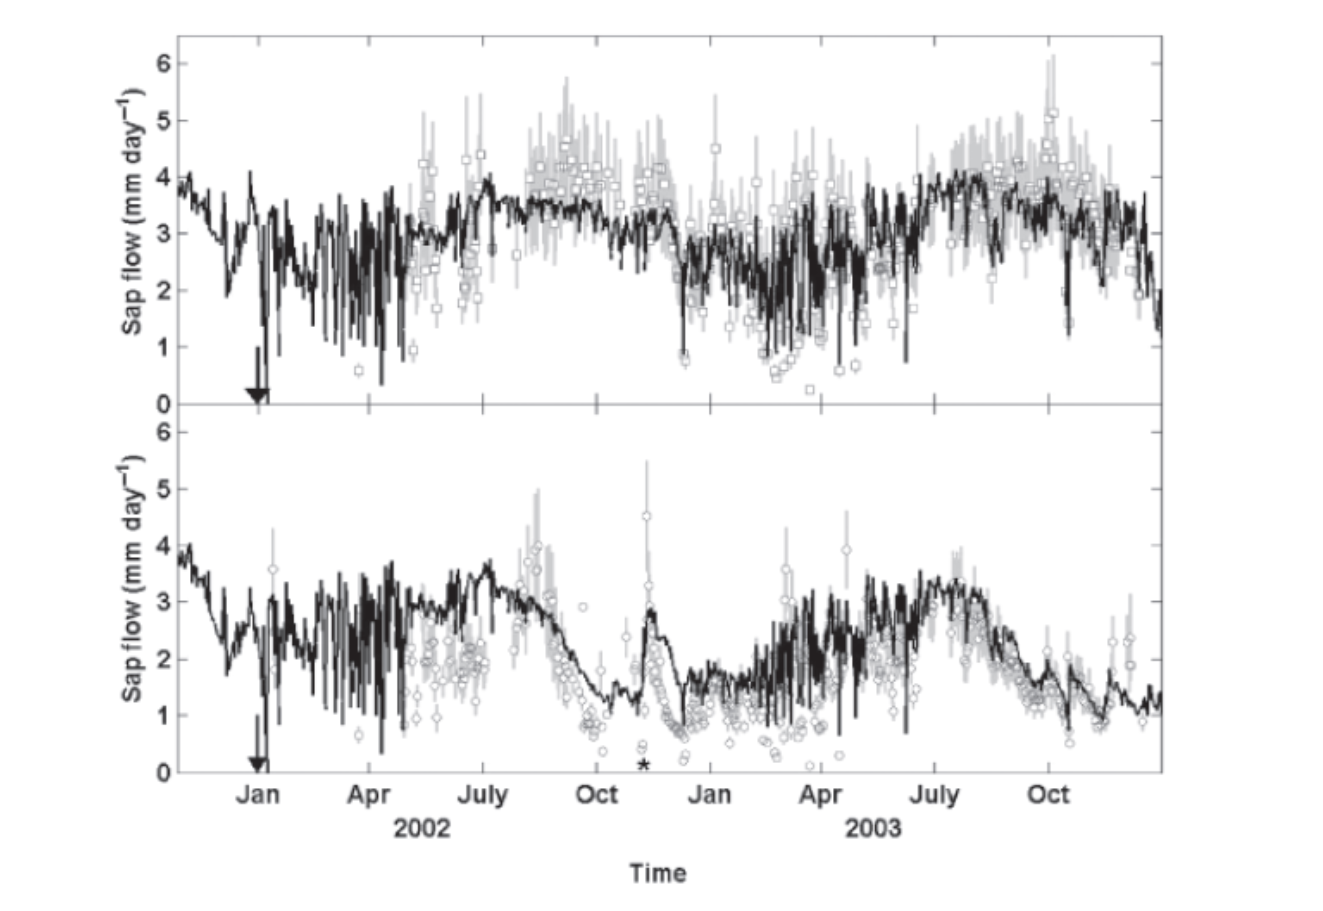
\includegraphics[width=0.8\linewidth]{figures/chap2/fisher1} 

}

\caption{Simulated (SPA model) and observed sapflow for a drought experiment in the Amazon; Fisher et al. 2007}\label{fig:f224}
\end{figure}

\begin{figure}

{\centering 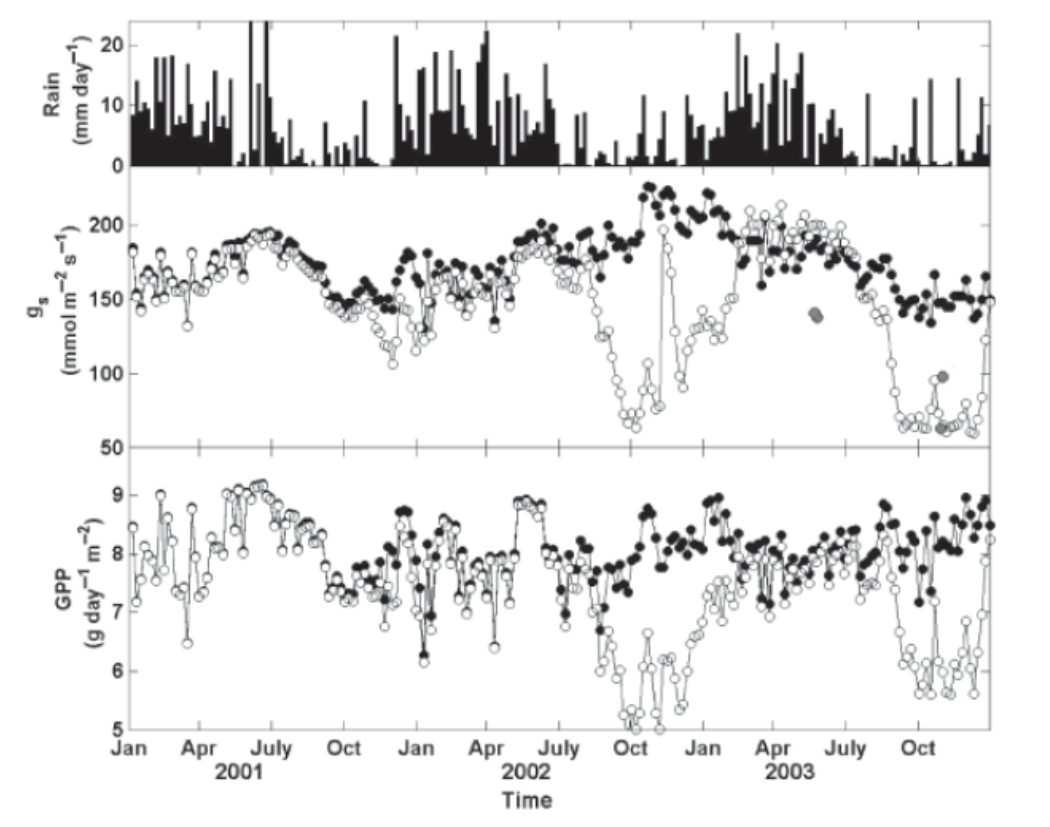
\includegraphics[width=0.8\linewidth]{figures/chap2/fisher2} 

}

\caption{Simulated (SPA model) gs and GPP for a drought experiment in the Amazon. Fisher et al. 2007}\label{fig:f225}
\end{figure}

\chapter{Modelling radiation, vegetation canopies, and energy
balance}\label{modelling-radiation-vegetation-canopies-and-energy-balance}

\chaptermark{Light}

\section{Introduction}\label{introduction}

\begin{figure}

{\centering 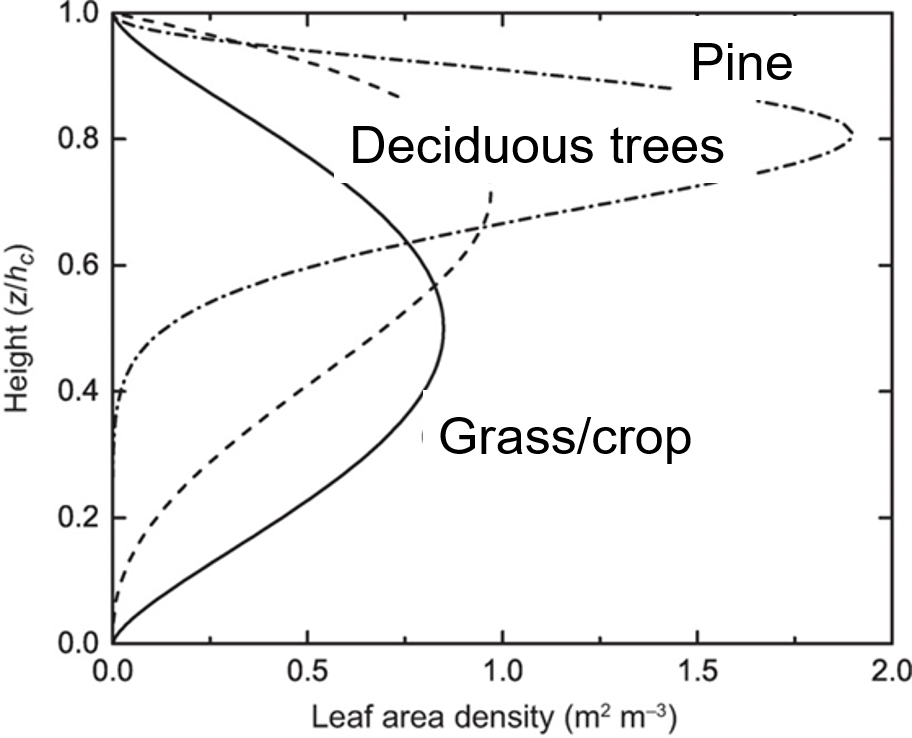
\includegraphics[width=0.8\linewidth]{figures/chap3/f31_LAD} 

}

\caption{Generalized profiles of leaf area density in plant canopies. (Bonan)}\label{fig:f31}
\end{figure}

\begin{figure}

{\centering 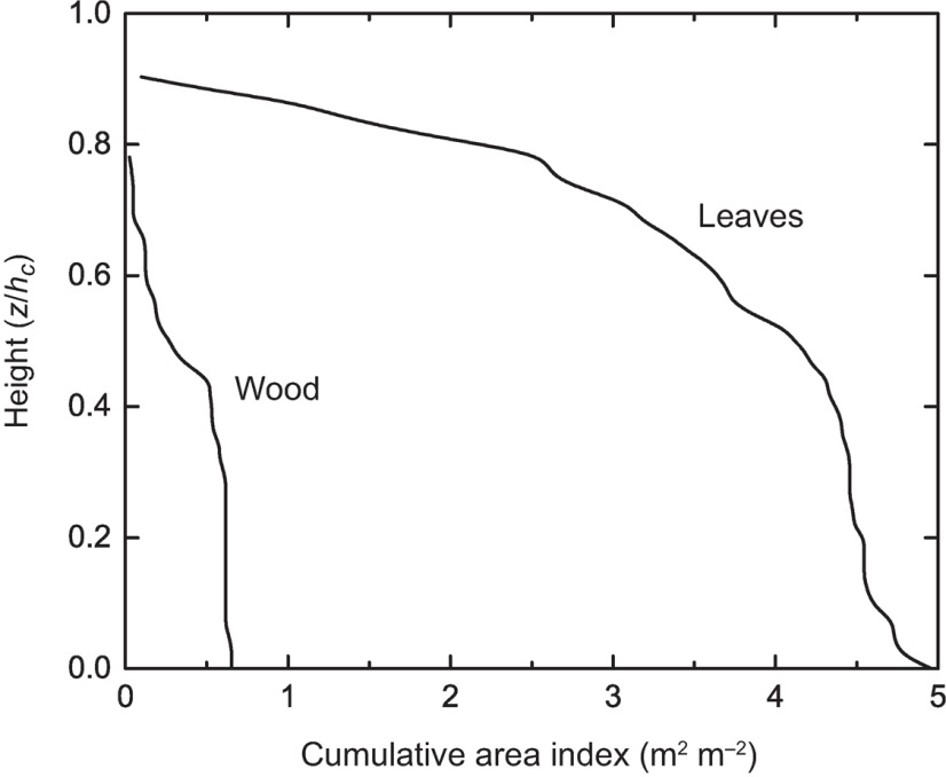
\includegraphics[width=0.8\linewidth]{figures/chap3/f32_cLAI} 

}

\caption{Cumulative LAI and WAI in a deciduous oak-hickory forest. (Bonan)}\label{fig:f32}
\end{figure}\begin{figure}

{\centering 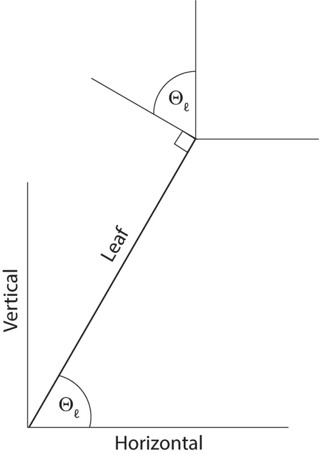
\includegraphics[width=0.8\linewidth]{figures/chap3/f33_Langle} 

}

\caption{Illustration of a leaf (thick line) oriented at an angle Θℓ to horizontal. (Bonan)}\label{fig:f33}
\end{figure}

\begin{figure}

{\centering 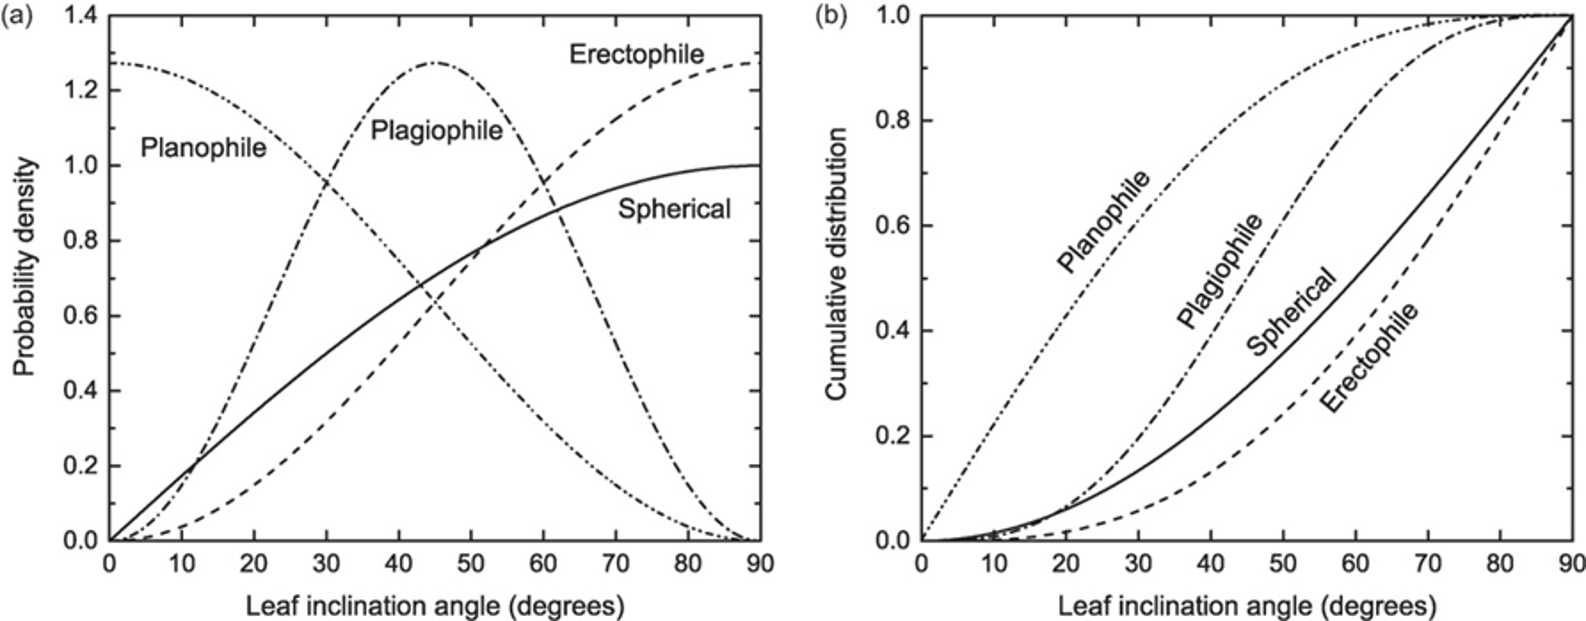
\includegraphics[width=0.8\linewidth]{figures/chap3/f34_angle_distr} 

}

\caption{Planophile, erectophile, plagiophile, and spherical leaf angle distributions showing (a) the probability density function f(Θℓ) and (b) the cumulative distribution F(Θℓ). (Bonan)}\label{fig:f34}
\end{figure}

\begin{figure}

{\centering 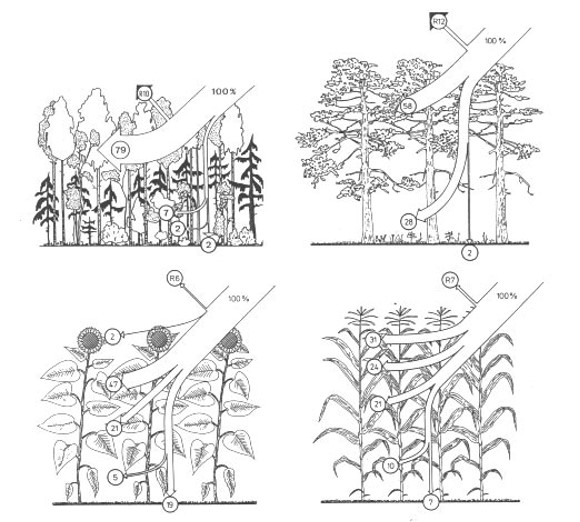
\includegraphics[width=0.8\linewidth]{figures/chap3/f35_architecture} 

}

\caption{Illustration of leaf angle distributions and canopy architecture in general influences radiation attenuation in vegetation canopies.}\label{fig:f35}
\end{figure}

\begin{figure}

{\centering 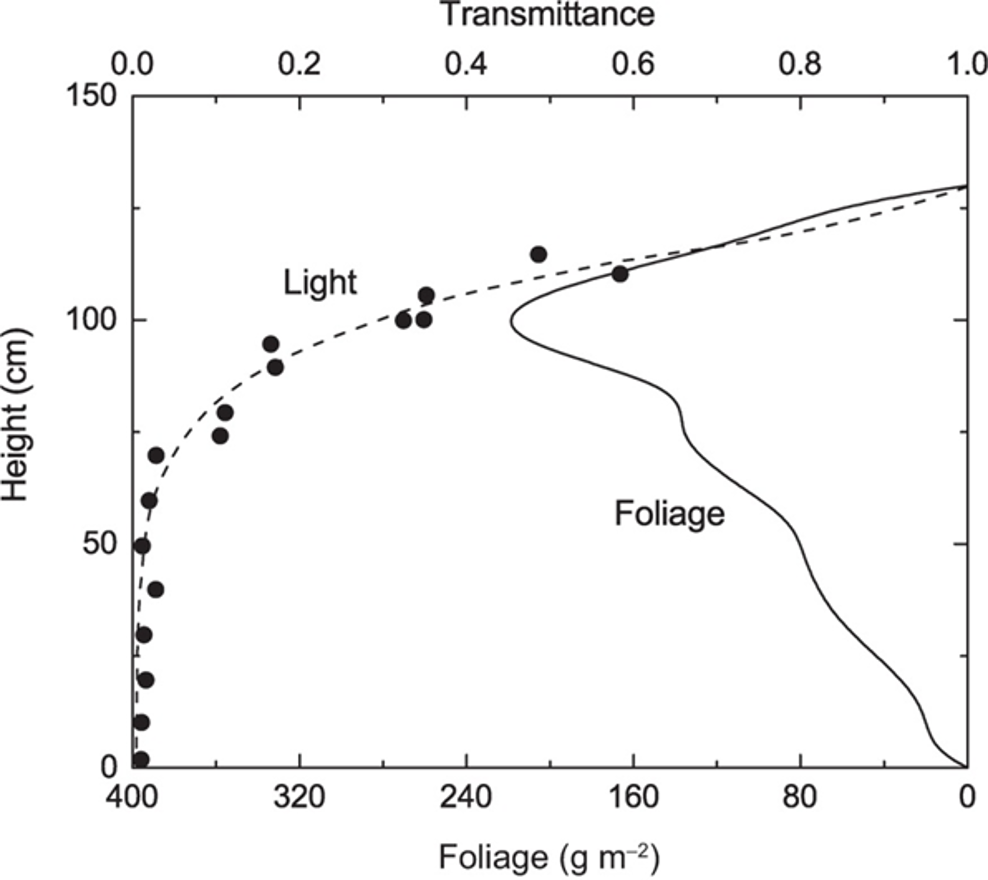
\includegraphics[width=0.8\linewidth]{figures/chap3/f36_obs_profile} 

}

\caption{Profile of light and foliage in a stand of herbaceous plants approximately 130 cm tall. The horizontal axis shows transmittance as a fraction of incident radiation (top axis) and foliage mass (bottom axis) at various heights in the canopy. (Bonan)}\label{fig:f36}
\end{figure}

\section{Radiative transfer
modelling}\label{radiative-transfer-modelling}

\begin{figure}

{\centering 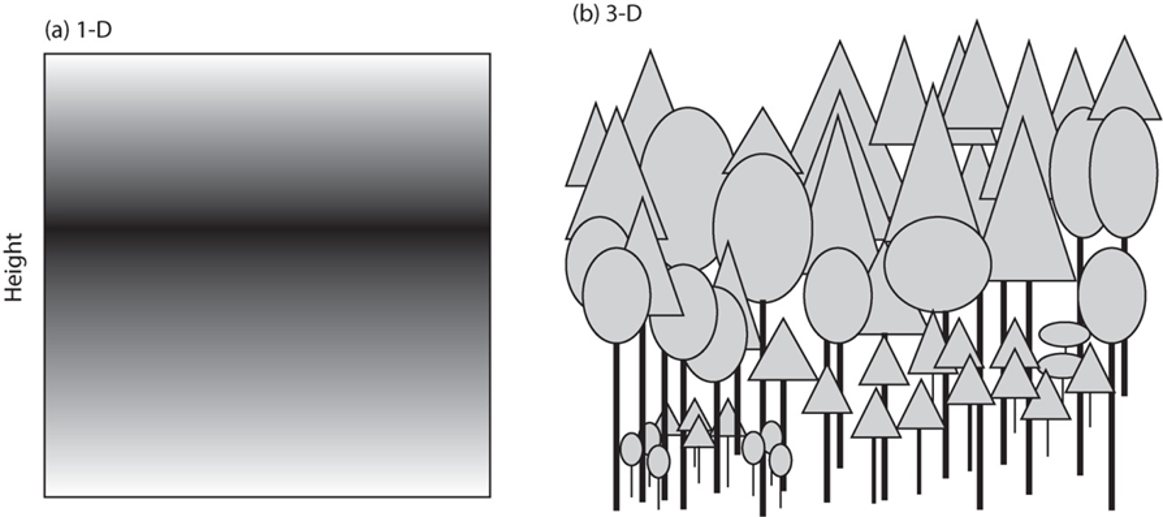
\includegraphics[width=0.8\linewidth]{figures/chap3/f37_RT_principle} 

}

\caption{Representation of a canopy as (a) one-dimensional with a vertical profile of leaf area (shown by grayscale gradation in which darker shading denotes more leaves) that is horizontally homogenous and (b) threedimensional with vertical and spatial structure determined by crown geometry and spacing. (Bonan)}\label{fig:f37}
\end{figure}

\subsection{Leaf optical properties}\label{leaf-optical-properties}

\begin{figure}

{\centering 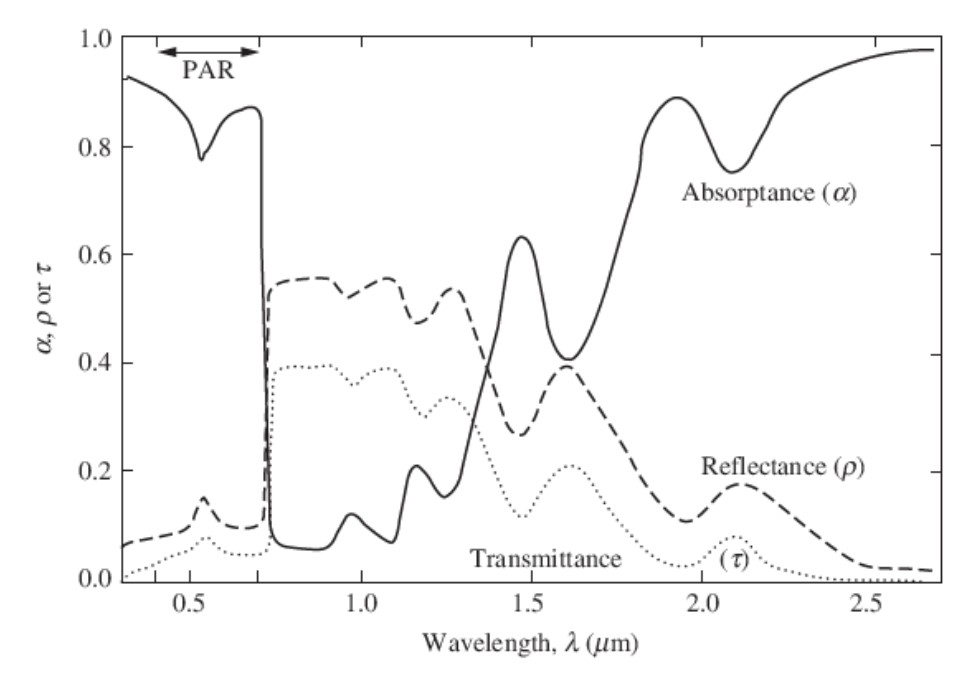
\includegraphics[width=0.8\linewidth]{figures/chap3/f37_leaf_optical} 

}

\caption{Spectrum of absorptance, reflectance and transmittance of a typical plant leaf (Jones, 2014)}\label{fig:f37b}
\end{figure}

\begin{figure}

{\centering \includegraphics[width=0.8\linewidth]{figures/chap3/f38_table_optical} 

}

\caption{Table showing typical reflectance and absorptance values for leaves and vegetation canopies of different Plant Functional Types (PFT).(Jones, 2014)}\label{fig:f38}
\end{figure}

\subsection{Light transmission without
scattering}\label{light-transmission-without-scattering}

\begin{figure}

{\centering \includegraphics[width=0.8\linewidth]{figures/chap3/f39_beer} 

}

\caption{Transmission of solar radiation through a homogeneous medium in the absence of scattering. In this example, n non-overlapping opaque particles each with cross-sectional area a oriented perpendicular to the path of light are placed in a medium with cross-sectional area A and thickness dz. The radiation absorbed in the medium is dI.(Bonan)}\label{fig:f39}
\end{figure}

\begin{figure}

{\centering \includegraphics[width=0.8\linewidth]{figures/chap3/f310_Kb} 

}

\caption{Transmission of direct beam radiation τb in relation to leaf area index for typical values of the extinction coefficient Kb. (Bonan)}\label{fig:f310}
\end{figure}

\begin{figure}

{\centering \includegraphics[width=0.8\linewidth]{figures/chap3/f311_LLh} 

}

\caption{Extinction coefficient in relation to solar zenith angle Ζ and leaf inclination angle Θℓ. In each panel, a unit leaf area (L = 1), shown with a thick line, is projected onto a horizontal surface LH so that Kb = LH. The leaf inclination angle is 0° (bottom panels), 30° (middle panels), and 60° (top panels). In the left and middle columns, the leaf is oriented towards the Sun (Αℓ − Α = 0°) and the solar zenith angle is 0° (left column) and 15° (middle column). In the right column, Ζ = 15°, but the leaf is oriented away from the Sun (Αℓ − Α = 180°). In each panel, the arrows indicate the solar beam (Bonan)}\label{fig:f311}
\end{figure}

\begin{figure}

{\centering \includegraphics[width=0.8\linewidth]{figures/chap3/f312_Kb_angle} 

}

\caption{Extinction coefficients for horizontal, spherical, and vertical leaf angle distributions. (a) Direct beam radiation Kb in relation to solar zenith angle. (b) Diffuse radiation Kd in relation to leaf area index(Bonan)}\label{fig:f312}
\end{figure}

\begin{figure}

{\centering \includegraphics[width=0.8\linewidth]{figures/chap3/f313_sun_shade} 

}

\caption{Radiative transfer and sunlit leaf area index for a canopy of horizontal leaves (top panels) with Kb = 1 and vertical leaves (bottom panels) with Kb = 0.112. The left-hand panels show a canopy consisting of four layers of leaves. Each thick black line represents a leaf area index of 0.1 m2 m–2. The thin lines depict interception or transmission of beam radiation with a zenith angle of 10°. The middle panels show cumulative leaf area index and sunlit leaf area index with depth in the canopy. The right-hand panels show direct beam transmittance with depth in the canopy. (Bonan)}\label{fig:f313}
\end{figure}

\begin{figure}

{\centering \includegraphics[width=0.8\linewidth]{figures/chap3/f314_sunlit} 

}

\caption{Sunlit leaf area index in relation to total leaf area index for horizontal, spherical, and vertical foliage orientations with solar zenith angle Ζ = 30°. Kb = 1, 0.577, and 0.368 for horizontal, spherical, and vertical foliage. (Bonan)}\label{fig:f314}
\end{figure}

\begin{figure}

{\centering \includegraphics[width=0.8\linewidth]{figures/chap3/f315_clumping} 

}

\caption{Images illustrating leaf/canopy clumping a various scales: leaf, crown, stand.}\label{fig:f315}
\end{figure}

\subsection{Diffuse transmittance}\label{diffuse-transmittance}

\begin{figure}

{\centering \includegraphics[width=0.8\linewidth]{figures/chap3/f316_diffuse} 

}

\caption{Illustration of direct beam and diffuse radiation. The sky forms a bowl, or inverted hemisphere, over a horizontal surface. Shown is a cross section of the sky hemisphere. Direct beam (solid line) originates from the    direction of the Sun with zenith angle Ζ. Diffuse radiation (dashed lines) can be treated as independent beams of radiation each with an angle Ζ. The shaded region is the relative contribution between sky angles Ζ1 and Ζ2 to total sky irradiance.(Bonan)}\label{fig:f316}
\end{figure}

\begin{figure}

{\centering \includegraphics[width=0.8\linewidth]{figures/chap3/f317_diff_trans} 

}

\caption{Transmittance of diffuse radiation τd in relation to leaf area index for a spherical leaf distribution. Show are the transmittances for sky zones of 0°–30°, 30°–60°, and 60°–90° and also the total transmittance. Fill patterns show the contribution of each sky zone to total transmittance.(Bonan)}\label{fig:f317}
\end{figure}

\begin{figure}

{\centering \includegraphics[width=0.8\linewidth]{figures/chap3/f318_diff_dir_trans} 

}

\caption{Transmission of solar radiation through a canopy with spherical leaf distribution in relation to leaf area index. The solid lines show direct beam transmittance τb for solar zenith angles of 0°–80° (in 10° increments).The dashed line shows the diffuse transmittance τd. (Bonan)}\label{fig:f318}
\end{figure}

\subsection{The Norman Model(1979)}\label{the-norman-model1979}

\begin{figure}

{\centering \includegraphics[width=0.8\linewidth]{figures/chap3/f319_Norman} 

}

\caption{Radiative fluxes in a canopy of N leaf layers. The vertical profile is oriented with i = 1 the leaf layer at the bottom of the canopy, leaf layer i + 1 above layer i, and i = N the leaf layer at the top of the canopy. Each layer has a leaf area index ΔL. is the downward diffuse shortwave flux onto layer i, is the upward diffuse shortwave flux above layer i, and is the unscattered direct beam flux onto layer i. and are the corresponding downward and upward fluxes of longwave radiation. These depend on leaf Tℓand ground Tg temperatures. Thick arrows denote boundary conditions of diffuse solar radiation , direct beam solar radiation, and atmospheric longwave radiation at the top of the canopy.(Bonan)}\label{fig:f319}
\end{figure}

\subsection{The Goudriaan and van Laar Model
(1994)}\label{the-goudriaan-and-van-laar-model-1994}

\begin{figure}

{\centering \includegraphics[width=0.8\linewidth]{figures/chap3/f320_goudriaan} 

}

\caption{ Derivation of absorbed direct beam solar radiation for a leaf layer with leaf area index ΔL (Goudriaan 1982). ρc is the reflectance of the leaf layer.(Bonan)}\label{fig:f320}
\end{figure}

\subsection{The Two-Stream
approximation}\label{the-two-stream-approximation}

\begin{figure}

{\centering \includegraphics[width=0.8\linewidth]{figures/chap3/f321_two_stream} 

}

\caption{Fluxes for (a) direct beam and (b) diffuse radiation in the twostream approximation for a canopy with leaf area index L.(Bonan)}\label{fig:f321}
\end{figure}

\subsection{Longwave radiation}\label{longwave-radiation}

\begin{figure}

{\centering \includegraphics[width=0.8\linewidth]{figures/chap3/f322_LW} 

}

\caption{Longwave radiation fluxes represented for a single leaf layer.(a) Norman’s (1979) numerical model. Shown is the radiative balance for leaf layer i + 1 located above leaf layer i. (b) A simplified model to allow only forward scattering (ρℓ = 0 and τℓ = ωℓ = 1 − εℓ) and to permit an analytical solution integrated over a canopy. In both panels, emitted radiation is excluded. Thick lines denote fluxes incident onto the layer. (Bonan)}\label{fig:f322}
\end{figure}

\section{Representing canopy structure in
models}\label{representing-canopy-structure-in-models}

\subsection{Big-leaf models}\label{big-leaf-models}

\begin{figure}

{\centering \includegraphics[width=0.8\linewidth]{figures/chap3/f323_bigleaf} 

}

\caption{Scaling of leaf fluxes to the canopy using a big-leaf model. (a) Shown are leaf sensible heat, transpiration, and CO2 fluxes in relation to various conductances. Fluxes are exchanged between the leaf and air around the leaf. Also shown is the total resistance. (b) Shown are big-leaf canopy fluxes in which leaf fluxes are scaled by the average conductance and leaf area index and are further modified by turbulent transport in the atmospheric surface layer. Surface layer processes are commonly omitted for CO2 exchange. Only a single big leaf is shown, but separate sunlit and shaded big leaves can be similarly depicted. (Bonan)}\label{fig:f323}
\end{figure}

\begin{figure}

{\centering \includegraphics[width=0.8\linewidth]{figures/chap3/f324_vcamx_profile} 

}

\caption{Canopy profiles of relative photosynthetic capacity in relation to cumulative leaf area index. Thin lines show exponential profiles using values of Kn for 16 temperate broadleaf forests and two tropical forests ranging from 0.10 to 0.43 (Lloyd et al. 2010). The two thick lines show observed profiles of Vcmax and Jmax from Niinemets and Tenhunen (1997) obtained for sugar maple (Acer saccharum). (Bonan)}\label{fig:f324}
\end{figure}

\subsection{Multilayer models}\label{multilayer-models}

\begin{figure}

{\centering \includegraphics[width=0.8\linewidth]{figures/chap3/f325_multilayer_process} 

}

\caption{Overview of the main processes in a multilayer canopy model.The canopy is represented by N leaf layers with layer i + 1 above layer i. (a) Diffuse and direct beam solar radiation is transmitted or intercepted. The intercepted portion is absorbed or scattered in the forward and backward direction. Longwave radiation is similar to diffuse radiation. (b) Leaf sensible heat, transpiration, and CO2 fluxes depend on absorbed radiation and leaf boundary layer and stomatal conductances. Sensible heat is exchanged from both sides of the leaf. Water vapor and CO2 can be exchanged from one or both sides of the leaf depending on stomata. Leaf temperature is the temperature that balances the energy budget. (c) Stomatal conductance depends on leaf water potential. Plant water uptake for a canopy layer is in relation to belowground soil and root conductance and aboveground stem conductance acting in series and also a capacitance term. See Figure 13.4a for more details. (d) Scalar profiles are calculated from a conductance network. Leaf fluxes provide the source or sink of heat, water vapor, and CO2, along with soil fluxes. (e) Sensible heat, latent heat, and heat storage in soil depend on the ground temperature that balances the soil energy budget. (f) The wetted fraction of the canopy layer depends on the portion of precipitation that is intercepted. (Bonan)}\label{fig:f325}
\end{figure}

\begin{figure}

{\centering \includegraphics[width=0.8\linewidth]{figures/chap3/f326_multilayer_solving} 

}

\caption{Flow diagram of processes in a multilayer canopy model. The shaded area denotes leaf processes resolved at each layer in the canopy. This is a generalized diagram of the required calculations for a dry leaf. Specific models differ in how the equation set is solved and the iterative calculations. Evaporation of intercepted water requires additional complexity.(Bonan)}\label{fig:f326}
\end{figure}

\subsection{3D ray tracing models}\label{d-ray-tracing-models}

\begin{figure}

{\centering \includegraphics[width=0.8\linewidth]{figures/chap3/f327_DART} 

}

\caption{Example of the PROSPECT leaf optical model and the DART 3D ray tracing model.}\label{fig:f327}
\end{figure}

\begin{figure}

{\centering \includegraphics[width=0.8\linewidth]{figures/chap3/f328_TLS_RT} 

}

\caption{Example of a study that uses terrestrial laser scanning (TLS) to construct a full 3D model of a forest as input for a 3D ray tracing model (Kükenbrink et al. 2020) }\label{fig:f328}
\end{figure}

\section{Ecosystem energy balance}\label{ecosystem-energy-balance}

\subsection{Basic principles}\label{basic-principles}

\subsection{Surface radiation balance}\label{surface-radiation-balance}

\begin{figure}

{\centering \includegraphics[width=0.8\linewidth]{figures/chap3/f329_rad_balance} 

}

\caption{Radiative balance of an opaque gray body receiving downwelling solar S↓ and longwave L↓ radiation.(Bonan)}\label{fig:f329}
\end{figure}

\subsection{Bulk surface energy
balance}\label{bulk-surface-energy-balance}

\begin{figure}

{\centering \includegraphics[width=0.8\linewidth]{figures/chap3/f330_E_balance} 

}

\caption{Conductance networks for sensible heat flux (top) and latent heat flux (bottom) for various depictions of the land surface. This chapter describes the bulk surface and big-leaf canopies. (Bonan)}\label{fig:f330}
\end{figure}

\subsection{Leaf energy balance}\label{leaf-energy-balance}

\begin{figure}

{\centering \includegraphics[width=0.8\linewidth]{figures/chap3/f331_leaf_E_balance} 

}

\caption{Biophysics and biochemistry of leaves. (a) The radiative environment consists of solar radiation (left) and longwave radiation (right). (b) Leaf fluxes include CO2, H2O, and heat through the boundary layer. These fluxes are shown as a network of conductances for the adaxial (upper) and abaxial (lower) leaf surfaces. For H2O and CO2, the conductance for each surface is obtained from stomatal and boundary layer conductances acting in series. The total conductance is defined by the adaxial and abaxial surfaces acting in parallel. (c) Stomata open to absorb CO2 for photosynthesis, but, in doing so, water is lost as transpiration. (Bonan)}\label{fig:f331}
\end{figure}

\section{Case studies}\label{case-studies-1}

\subsection{Case study 3.1}\label{case-study-3.1}

\begin{figure}

{\centering \includegraphics[width=0.8\linewidth]{figures/chap3/f332_knohl1} 

}

\caption{Principle of the effect of increased diffuse raditaion on leaf/canopy photosynthesis. (Knohl et al. 2008)}\label{fig:f332}
\end{figure}

\begin{figure}

{\centering \includegraphics[width=0.8\linewidth]{figures/chap3/f333_knohl2} 

}

\caption{Resulting impact of changing diffuse fraction on carbon and water fluxes and WUE (Knohl et al. 2008)}\label{fig:f333}
\end{figure}

\subsection{Case study 3.2}\label{case-study-3.2}

\begin{figure}

{\centering \includegraphics[width=0.8\linewidth]{figures/chap3/f334_chen1} 

}

\caption{Global map of LAI trend between 1981 and 2016 based on remote sensing (Chen et al. 2021).}\label{fig:f334}
\end{figure}

\begin{figure}

{\centering \includegraphics[width=0.8\linewidth]{figures/chap3/f335_chen2} 

}

\caption{Simulated impact of different factors contributing to the increased global land C sink since 1981 (Chen et al. 2021) }\label{fig:f335}
\end{figure}

\chapter{Modelling temporal and seasonal
dynamics}\label{modelling-temporal-and-seasonal-dynamics}

\chaptermark{dynamics}

\section{Introduction on temporal
dynamics}\label{introduction-on-temporal-dynamics}

\begin{figure}

{\centering \includegraphics[width=0.8\linewidth]{figures/chap4/f41_Krinner} 

}

\caption{Evaluation of the temporal dynamics of fluxes (Rn: Net Radiation, H: sensible heat, LE: latent heat, NEE: net ecosystem exchanges of CO2) simulated by the global model ORCHIDEE. LEFT: measured (color) and modelled "summer" diurnal cycle for each flux and each PFT. RIGHT: measured (color) and modelled seasonal cycle for each flux and each PFT. (Krinner et al. 2005)}\label{fig:f41}
\end{figure}

\section{Phenology: the background}\label{phenology-the-background}

\begin{figure}

{\centering \includegraphics[width=0.8\linewidth]{figures/chap4/f42_Defilia} 

}

\caption{Larch needle appearance in Sargans 1958-2002. Dashed line is trend 1958-1999, solid line is trend 1958-2002.  (Defilia and Clot 2005)}\label{fig:f42}
\end{figure}

\begin{figure}

{\centering \includegraphics[width=0.8\linewidth]{figures/chap4/f43_Polgar} 

}

\caption{Concept of various effect that changing phenology can have on ecosystem processes (e.g. productivity or transpiration). (Polgar and Primack 2011)}\label{fig:f43}
\end{figure}

\section{Leaf phenology models}\label{leaf-phenology-models}

\subsection{Prescribed phenology}\label{prescribed-phenology}

\begin{figure}

{\centering \includegraphics[width=0.8\linewidth]{figures/chap4/f44_zhang} 

}

\caption{Sample time series of MODIS EVI data and estimate phenological transition dates for a mixed forest pixel in New England. Diamonds: EVI data, solid line with stars: fitted logistic model. (Zhang et al. 2003)}\label{fig:f44}
\end{figure}

\begin{figure}

{\centering \includegraphics[width=0.8\linewidth]{figures/chap4/f45_zhang_map} 

}

\caption{Maps of phenological transition dates for New England. (Zhang et al. 2003)}\label{fig:f45}
\end{figure}

\subsection{Budburst models}\label{budburst-models}

\subsection{Snescence models}\label{snescence-models}

\subsection{Leaf age}\label{leaf-age}

\begin{figure}

{\centering \includegraphics[width=0.8\linewidth]{figures/chap4/f46_vc_age} 

}

\caption{Relation  between Vcmax and leaf age in the ED2 vegetation model. (Kim et al. 2011)}\label{fig:f46}
\end{figure}

\subsection{Phenology in DGVMs}\label{phenology-in-dgvms}

\subsection{Phenology in the tropics}\label{phenology-in-the-tropics}

\begin{figure}

{\centering \includegraphics[width=0.8\linewidth]{figures/chap4/f49_junglerythms} 

}

\caption{Example of how manual historical phenology observations in Yangambi (DR Congo) are trasnlated in a visual phenology pattern for a single tree species. (junglerythms.org))}\label{fig:f49}
\end{figure}

\textbackslash{}begin\{figure\}

\{\centering \includegraphics[width=0.8\linewidth]{figures/chap4/f410_kearsley}

\}

\textbackslash{}caption\{Overview of species-specific timing of onset of
leaf phenophases for evergreen and deciduous species in tropical forest
in Yangambi (DR Congo). The median timing of the onset of leaf
senescence and turnover is indicated for each species. Species-specific
bootstrapped 95\%-confidence intervals are indicated with a line
segment. Species are arranged according to the variability in the timing
of the phenophase, with species with the lowest uncertainty at the outer
edge and continuing towards the center. Species with an annual (full
circles) or sub-annual (crosses) fourier-based seasonality are
indicated. Grey shaded areas represent the average timing of the long
and short dry seasons (LD and SD; monthly precipitation \textless{} 150
mm), separated by the long and short wet seasons (LW and SW). (Kearsley
et al. 2021))\}\label{fig:f410} \textbackslash{}end\{figure\}

\section{Case studies}\label{case-studies-2}

\subsection{Case study 4.1}\label{case-study-4.1}

\begin{figure}

{\centering \includegraphics[width=0.8\linewidth]{figures/chap4/f47_LAI_richardson} 

}

\caption{Simulated and observed LAI for 5 deciduous forest sites and 14 vegetation models participating to the NACP model intercomparison project. (Richardson et al. 2012)}\label{fig:f47}
\end{figure}

\begin{figure}

{\centering \includegraphics[width=0.8\linewidth]{figures/chap4/f48_bias_richardson} 

}

\caption{Bias in modeled gross ecosystem photosynthesis (GEP=GPP) for deciduous broadleaf (top) and evergreen needleleaf (bottom) forests. Left panels show bias, by model. Right panels show the frequency distribution of these spring and autumn biases in re-scaled model GEP, across all models, sites, and years of data, for each forest type. The sign convention is that positive bias means that modeled GEP > tower GEP. (Richardson et al. 2012)}\label{fig:f48}
\end{figure}

\subsection{Case study 4.2}\label{case-study-4.2}

\begin{figure}

{\centering \includegraphics[width=0.8\linewidth]{figures/chap4/f411_chen1} 

}

\caption{Observed and assumed relation between Vcmax and leaf age in the ORCHIDEE global model, for the tropical evergreen PFT. (Chen et al. 2018)}\label{fig:f411}
\end{figure}

\begin{figure}

{\centering \includegraphics[width=0.8\linewidth]{figures/chap4/f412_chen2} 

}

\caption{Comparison of litterfall data with two new and the old leaf turnover schemes in the ORCHIDEE model for 4 sites in the Amazon. (Chen et al. 2018)}\label{fig:f412}
\end{figure}

\begin{figure}

{\centering \includegraphics[width=0.8\linewidth]{figures/chap4/f413_chen3} 

}

\caption{Comparison of GPP fluxtower data with two new and the old leaf turnover schemes in the ORCHIDEE model for 4 sites in the Amazon. (Chen et al. 2018)}\label{fig:f413}
\end{figure}

\part{Modelling vegetation
dynamics}\label{part-modelling-vegetation-dynamics}

\chapter{Modelling plant growth and biogeochemical cycles in vegetation
models}\label{modelling-plant-growth-and-biogeochemical-cycles-in-vegetation-models}

\chaptermark{Grotwh} - UCL 4.2.2

based on Bonan Chapter 17

\section{Process-based growth
modelling}\label{process-based-growth-modelling}

\subsection{C-allocation models}\label{c-allocation-models}

\begin{itemize}
\tightlist
\item
  C pools: Allocation to leaf, wood, fruit
\end{itemize}

\subsection{Applications of growth modelling in forestry and
agriculture}\label{applications-of-growth-modelling-in-forestry-and-agriculture}

\begin{itemize}
\tightlist
\item
  short, link with inventory course
\end{itemize}

\section{Carbon cycle models: stocks and
fluxes}\label{carbon-cycle-models-stocks-and-fluxes}

This chapter will develop the ecological foundation and mathematics to
describe ecosystem carbon dynamics using biogeochemical models.
Biogeochemical models abstract an ecosystem as pools of carbon and the
flows of carbon among these pools.

Use specific model as an example to illustrate? In Bonan: CASA-CNP model

\subsection{Model structure}\label{model-structure}

Biogeochemical models simulate processes of allocation of photosynthetic
carbon gain to plant parts (e.g., foliage, fine root, wood), turnover of
plant biomass as litterfall, transformation of litter to soil organic
matter, and carbon loss during respiration.

Principles: - net carbon input is equal to gross primary production
minus autotrophic respiration; - carbon flows from donor to receiver
pools at a rate that depends on the donor pool size and its chemical
quality as modified by the environment; - mass balance is maintained as
carbon flows through the system of interconnected pools; - decay of
litter and soil organic matter releases CO 2 as heterotrophic
respiration.

Models: a system of first-order, linear differential equations to
describe carbon pools and fluxes (typically time step of one day)

Pools and fluxes to be included: - Carbon gain from gross primary
production minus autotrophic respiration - Allocation of carbon to
growth of leaves, wood, and roots pools (partitioning varies with light
availability, soil temperature, soil moisture, and nutrients + temporal
for leaves (ref to phenology) - Carbon turnover (comprising litterfall,
background mortality, and disturbances) + turnover rates depending on
the plant material - litter pools: metabolic litter, structural litter,
coarse woody debris (vary in chemical quality and turnover rate; base
turnover rates are modified for soil temperature and soil moisture
(environmental scaling factors)) - decomposition to soil organic matter
pools: fast SOM, slow SOM, passive SOM (vary in chemical quality and
turnover time) - portion of the decomposition flow lost as heterotrophic
respiration

Bonan - Figure 17.2: structure of a typical biogeochemical model -
equations 17.1 -- 17.10

Additional details? - maintenance respiration and growth respiration -
storage pool of nonstructural carbohydrates - some models separate wood
into live stems (sapwood) and dead stems, roots into fine roots and
coarse roots, and coarse roots into live pools and dead pools to account
for the different physiological functioning of these biomass components

\subsection{Allocation and turnover
parameterization}\label{allocation-and-turnover-parameterization}

\begin{itemize}
\item
  types of allocation models (see Campioli et al 2013 and work of
  Fatichi et al. )
\item
  allocation parameters
\item
  fixed allocation and dynamic allocation (specified by biome or based
  on environmental conditions)
\item
  Optimality models: plants optimally allocate resources to balance
  light acquisition (foliage), structural support and water transport
  (stems), and water and nutrient uptake (roots).
\item
  allocation based on scaling relationships among plant components
  (specified ratios of foliage, root, and wood biomass)
\item
  Turnover rates vary depending on plant material and are specified as a
  fraction of biomass.
\item
  Turnover rates are commonly estimated as the inverse of residence time
  or longevity
\item
  biogeochemical models can be applied to any type of ecosystem such as
  grassland, savanna, forest, shrubland, and tundra
\end{itemize}

\section{Nutrient cycle models: soil biogeochemical
models}\label{nutrient-cycle-models-soil-biogeochemical-models}

\subsection{Nitrogen cycle}\label{nitrogen-cycle}

\begin{itemize}
\item
  Bonan Chapter 17.6 Nitrogen Cycle
\item
  Bonan Figure 17.8: Depiction of the nitrogen cycle
\item
  only \textasciitilde{}recently added in most biogeochemical models
\item
  closely coupled to carbon cycle
\item
  important role to limit plant productivity
\item
  similar to carbon with an associated nitrogen pool and transfer.
\item
  cycling of nitrogen can be represented by a system of linear
  differential equations similar to that for carbon.
\item
  allocation of plant nitrogen uptake up to plant pools
\item
  loss of nitrogen in litterfall + portion is reabsorbed
\item
  soil nitrogen cycle is more complex (various forms)
\item
  decomposition of litter and soil organic matter, (mineralization and
  immobilization)
\item
  nitrification, denitrification, leaching, ammonia volatilization
\item
  additional inputs from biological nitrogen fixation, atmospheric
  deposition, and fertilizer
\item
  some examples of models? CLM?
\item
  All models simulate a decrease in plant growth when soil mineral
  nitrogen is insufficient to meet demand, but they differ in the manner
  in which this is implemented.
\item
  maybe also more soil oriented model (CENTURY , \ldots{}.)
\item
  discuss different approaches?
\end{itemize}

\subsection{Phosphorus cycle}\label{phosphorus-cycle}

Not in Bonan - Some models additionally include phosphorus (Wang et al.
2010; Yang et al. 2014; Goll et al. 2017) - ORCHIDEE, CLM-CNP

\subsection{Other nutrients}\label{other-nutrients}

\begin{itemize}
\tightlist
\item
  K and Mg in Eucalyptus and other tropical plantations
\end{itemize}

\section{Water balance}\label{water-balance}

\begin{itemize}
\item
  focus on the surface energy balance and vertical water movement in the
  soil--plant atmosphere system (e.g., soil moisture control of
  evapotranspiration)
\item
  Specific components in terrestrial biosphere models:\\
  Interception, throughfall, stemflow, infiltration, surface runoff,
  soil water redistribution, subsurface runoff, snow melt, evaporation,
  transpiration, plant water uptake, stomatal conductance
\end{itemize}

\subsection{A bucket model hydrologic
cycle}\label{a-bucket-model-hydrologic-cycle}

\begin{itemize}
\tightlist
\item
  refer to hydrology courses in the program
\item
  change in soil water is the difference between precipitation and
  evapotranspiration, excess runs off
\item
  based on maximum water-holding capacity
\end{itemize}

\chapter{Representing biodiversity in vegetation
models}\label{representing-biodiversity-in-vegetation-models}

\chaptermark{Biodiversity}

\section{Why and how representing biodiversity in vegetation
models?}\label{why-and-how-representing-biodiversity-in-vegetation-models}

We can start with the applications? I think it is more interesting than
finishing with the applications. Application: Conservation, ecosystem
resilience, vegetation-atmosphere feedbacks

Biodiversity refers here to functional diversity.

\section{Functional diversity}\label{functional-diversity}

\begin{itemize}
\tightlist
\item
  check the book " Terrestrial Ecosystems in a changing world" from P.
  Canadell (2007)
\item
  Part C: Landscapes under changing disturbance regimes:

  \begin{itemize}
  \tightlist
  \item
    PFT
  \item
    Fire and disturbances
  \item
    upscalling
  \item
    construction, evaluation and examples of DGVM applications
  \end{itemize}
\end{itemize}

\subsection{Definition of funcional diversity and plant functional
traits}\label{definition-of-funcional-diversity-and-plant-functional-traits}

Any morphological, physiological or phenological feature measurable at
the individual level, from the cell to the whole-organism level, without
reference to the environment or any other level of organization. It is
functional if it affects fitness indirectly via its effects on growth,
reproduction and survival.

\begin{itemize}
\tightlist
\item
  Seminal papers from the plant functional trait community Violle 2007,
  Lavorel, garnier, Shipley, etc\ldots{}
\end{itemize}

\includegraphics{figures/Violle2007.jpg} - Mention here the interesting
summer school:
\url{http://www.cef-cfr.ca/index.php?n=MEmbres.AlisonMunsonPlantTraits?userlang=en}
- List of reference papers in the link above - 3 types of traits:
dynamic, response \& constant, that are linked to the processes we
studied in the previous chapter (slow/fast processes)

\subsection{Representing 400 000 plant species in a single model: the
Plant Functional Type
approach}\label{representing-400-000-plant-species-in-a-single-model-the-plant-functional-type-approach}

Short description in UCL 4.3.2\\
No description in Bonan

\begin{itemize}
\tightlist
\item
  Lack of observations for every species
\item
  Computing resources problem (refers to the history of DGVMs from the
  introduction)
\item
  A simplification based on biome description and plant functionning at
  the ecosystem level
\item
  Different definitions of PFT: statistical classification, etc.
\item
  Table of classical PFTs used in models here.
\item
  PFT mapping: multi-obs approach based on remote sensing.
\item
  First use of PFTs managed to reproduce well the gradients at the
  global scale, but now it is unsuficcient.
\end{itemize}

\subsection{Limits of the PFT representation in the context of global
change}\label{limits-of-the-pft-representation-in-the-context-of-global-change}

\begin{itemize}
\tightlist
\item
  Including acclimation and adaptation processes
\item
  Dynamic vegetation: Accounting for non-random species turnover
\item
  Quantifying vegetation-environment feedbacks
\item
  Quantifying impacts of biodiversity on ecosytem functioning and
  climate
\end{itemize}

\subsection{From model parameters to plant
traits}\label{from-model-parameters-to-plant-traits}

\begin{itemize}
\tightlist
\item
  Reconciliating modelling with functional ecology.
\item
  Existing databases (TRY)
\item
  Empirical approach: More PFTs with traits instead of model-specific
  parameters, trait-trait, trait-environment relationships
\item
  Trade-offs: modeling plant strategies --\textgreater{} LES, PES, RES,
  all the ES :D
\item
  Role of data assimilation in regions without data and to assess
  spatial variability of vegetation properties
\item
  But: requires lots of observations in space and time.
\end{itemize}

\subsection{Eco-evolutive optimality
approaches}\label{eco-evolutive-optimality-approaches}

\begin{itemize}
\tightlist
\item
  New generation of models
\item
  PPA, coordination, ect\ldots{}
\item
  Paper from Oskar.
\end{itemize}

\section{Competition models}\label{competition-models}

Not in Bonan nor UCL\\
In Bonan Chapter 19 on demography, gap models, etc\ldots{} which is a
part of competition.

\subsection{Representation of PFTs in vegetation
models}\label{representation-of-pfts-in-vegetation-models}

\begin{itemize}
\tightlist
\item
  Parameterization and calibration of PFTs--\textgreater{} data
  assimilation, traits, model-specific parameters
\item
  representation by pixels
\item
  shared processes, different processes
\item
  interaction between PFTs
\item
  Depend on the model: individual/cohort/big leaf
\end{itemize}

\subsection{Competition for ressources / Plant
strategy?}\label{competition-for-ressources-plant-strategy}

\begin{itemize}
\tightlist
\item
  In fact we can extend the trait based approach and plant strategy
  (PES, etc) in the competition and community section?
\item
  Mortality, turnover, etc..
\end{itemize}

\subsection{Representation of trait
distributions}\label{representation-of-trait-distributions}

\begin{itemize}
\tightlist
\item
  Trade-offs
\end{itemize}

\section{Communities}\label{communities}

\begin{itemize}
\tightlist
\item
  Successions and impact on cycles, species composition etc.
\end{itemize}

\section{What about crops?}\label{what-about-crops}

\begin{itemize}
\tightlist
\item
  Not our focus but we don't forget it. A few words to say that specific
  crop models exists
\item
  Diversity is not a problem anymore
\item
  Plant functional traits are still central to crop modelling, but
  competition and diversity are no more an issue.
\item
  Other problematics specific to agriculture, such as agro-ecosystems
  where we have multi layers of vegetation (Trees over crops)
  --\textgreater{} Very interesting modelling problem and application
  especially in arid/semi-arid and tropical regions
\end{itemize}

\chapter{Modelling vegetation dynamics and
demography}\label{modelling-vegetation-dynamics-and-demography}

\chaptermark{Dynamics}

Bonan Chapter 19.2 Another class of models, known as individual plant or
ecosystem demography models, retains the complexity of individual plants
or cohorts of similar plants. In these models, ecosystem properties such
as carbon storage are the outcome of demographic processes.

\begin{itemize}
\tightlist
\item
  plant populations
\item
  community composition
\item
  ecosystem structure
\item
  driven by demographic processes of recruitment, establishment, growth,
  and mortality
\end{itemize}

\section{Gap models, individual and cohort based
models}\label{gap-models-individual-and-cohort-based-models}

\begin{itemize}
\item
  small scale models; landscape represented as a mosaic of hundreds of
  independent forest patches, each of which can differ in species
  composition and stage of development in response to disturbance that
  creates an opening in the canopy
\item
  models track the establishment, growth, and death of individual trees
  in an area of land.
\item
  Each tree is characterized by its species, stem diameter, height, and
  age.
\item
  trees compete for light, soil moisture, and nutrients.
\item
  patch undergoes temporal changes in the density, size, and composition
  of trees with the formation of a gap in the canopy
\item
  Community composition, biomass, productivity, and biogeochemical
  cycles are emergent outcomes of individual trees interacting among
  themselves and with the environment to acquire the resources necessary
  for growth and survival
\item
  cohort-based models define patches based on age since disturbance and
  simulate the dynamics of cohorts of similar plant functional types
  rather than tracking every individual.
\item
  Common to each model is the representation of vegetation demography,
  with age- and size-dependent growth and mortality and in which growth
  is constrained by allometric relationships of stem diameter with
  height, sapwood area, leaf area, and biomass. cohort models
  --\textgreater{} modelling size distributions
\end{itemize}

\section{Allometric relationships}\label{allometric-relationships}

\begin{itemize}
\tightlist
\item
  link with growth modelling of previuous chapter
\item
  allometric relationships are a critical driver of individual tree
  growth.
\item
  Height is important for its effect on stem diameter increment, both
  directly through tree volume growth and indirectly through shading.
\item
  Biomass allocation: empirical equations that constrain foliage, stem,
  and root mass for a given size tree
\item
  relationship between stem diameter and leaf area drives light
  extinction in the canopy
\item
  annual growth of a tree is calculated from its diameter and height as
  modified by light, climate, and site conditions. Growth curves figure
  19.5
\end{itemize}

\section{Competition for light}\label{competition-for-light}

\begin{itemize}
\tightlist
\item
  critical driver of forest dynamics
\item
  shading of smaller individuals by taller trees
\item
  vertical profile of leaf area in the patch (vertical structure in
  which trees are arranged into canopy layers)
\item
  height of a tree determines its location in the cumulative leaf area
  profile
\item
  light extinction coefficient
\item
  figure 19.6: representation of plant canopies
\end{itemize}

\section{Seed dispersal and
recruitment}\label{seed-dispersal-and-recruitment}

\begin{itemize}
\item
  regeneration: stochastic process
\item
  seeds of species are assumed to be present on-site
\item
  available light at the forest floor, climate tolerances, and other
  site conditions determine which species become established.
\item
  sprouting based on size
\item
  Species are characterized by life history characteristics + maybe add
  example of herb layer models of FORNALAB
\end{itemize}

\section{Mortality}\label{mortality}

\begin{itemize}
\item
  stochastic process
\item
  Trees die with a constant probability each year
\item
  The probability of mortality increases when tree growth is less than
  some minimum
\item
  disturbance related mortality : Wildfire and insect outbreaks can be
  included
\item
  The occurrence of fire is treated stochastically with an annual
  probability of burning. An individual patch may, for example, have a
  1\% change of burning in any given year.
\end{itemize}

\part{Upscaling and
applications}\label{part-upscaling-and-applications}

\chapter{Spatial heterogeneity, landscape scale,
metapopulations}\label{spatial-heterogeneity-landscape-scale-metapopulations}

\chaptermark{Heterogeneity}

\section{Patch dynamics}\label{patch-dynamics}

Some references: - Book: The ecology of natual disturance and patch
dynamics, Pickett \& White, 2013

\subsection{Spatial heterogeneity:
Definitions}\label{spatial-heterogeneity-definitions}

\begin{itemize}
\tightlist
\item
  Definition of Patch Dynamics, Perturbation, Disturbance:
\item
  Spatial heterogeneity
\item
  Resilience and shifts
\end{itemize}

\subsection{Impact of heterogeneity on ecosystem fonctionning and
environmental
feedbacks}\label{impact-of-heterogeneity-on-ecosystem-fonctionning-and-environmental-feedbacks}

\begin{itemize}
\tightlist
\item
  Show examples here of the impact of heterogeneity
\item
  Application in the design of nature reserves for example
\end{itemize}

\subsection{Heterogeneity is a matter of
resolution}\label{heterogeneity-is-a-matter-of-resolution}

\begin{itemize}
\tightlist
\item
  Imbricated levels of heterogeneity depending on spatial and temporal
  resolution
\item
  Heterogeneity is also a matter of the studied question: important in
  term of modelling since it will govern how processes are implemented
\end{itemize}

\subsection{Representation in Vegetation models: what are the drivers of
spatial
heterogeneity?}\label{representation-in-vegetation-models-what-are-the-drivers-of-spatial-heterogeneity}

\begin{itemize}
\tightlist
\item
  List here the different drivers
\item
  Heterogeneity is a patchwork of homogeneity in most models
\item
  But we can still represent dynamics in heterogeneity --\textgreater{}
  mortality, growth and shifts in species composition
\end{itemize}

\subsection{Disturbances and Patch
dynamics}\label{disturbances-and-patch-dynamics}

\begin{itemize}
\tightlist
\item
  We listed the different drivers above, we will now discuss in detail
  the most important aspects affecting patch dynamics
\item
  Link to land-use and disturbance
\end{itemize}

\section{Land-use changes}\label{land-use-changes}

\begin{itemize}
\tightlist
\item
  Land use is linked to spatial heterogeneity and patch dynamics
\end{itemize}

\subsection{Role of Land-use in global emissions and biogeochemicel
cycles}\label{role-of-land-use-in-global-emissions-and-biogeochemicel-cycles}

\begin{itemize}
\tightlist
\item
  impact C stocks and fluxes
\item
  impact on nutrients (depletion over rotations, etc\ldots{})
\item
  important impact on respiration
\item
  vegetation cover and biophysical impact: albedo, etc\ldots{}
\item
  Specific case of deforestation, one of the most important imapct (make
  a paragraph on that?)
\item
  How are fluxes attributed to land use in gas emission assessments?
  --\textgreater{} central role of vegetation modeling
\end{itemize}

\subsection{The important role of land use in the water
cycle}\label{the-important-role-of-land-use-in-the-water-cycle}

\begin{itemize}
\tightlist
\item
  Affects regional precipitations
\item
  Affects water routing --\textgreater{} Compared to the local impact on
  vegetation, here we touch something that will have an impact for the
  surrounding regions
\end{itemize}

\subsection{Monitoring land-use}\label{monitoring-land-use}

\begin{itemize}
\tightlist
\item
  remote sensing, rapid link to other courses
\end{itemize}

\subsection{How Land-use is represented in vegetation
models?}\label{how-land-use-is-represented-in-vegetation-models}

\begin{itemize}
\tightlist
\item
  Compared to vegetation dynamic which is process-based, here land use
  is imposed.
\item
  management
\item
  urban areas
\end{itemize}

\section{Natural and Anthropogenic
disturbances}\label{natural-and-anthropogenic-disturbances}

\begin{itemize}
\tightlist
\item
  We provide an overview of disturbances but we will detail only one of
  each: Fires and Management
\end{itemize}

\subsection{Wind and extrem events}\label{wind-and-extrem-events}

\begin{itemize}
\tightlist
\item
  Modelling storms
\item
  Modelling heat and cold waves, frost impact
\end{itemize}

\subsection{Herbivory}\label{herbivory}

\begin{itemize}
\tightlist
\item
  Yes herbivory is represented in vegetation models :D
\item
  Palability traits/ fixed fraction/ insects
\end{itemize}

\subsection{Modelling fires}\label{modelling-fires}

\begin{itemize}
\tightlist
\item
  In UCL Practical chap. 6
\item
  For estimating the impact on ecosystems
\item
  To be able to predict fires
\item
  Observation of fires and quantifications of fluxes
\item
  Fires and deposition
\item
  Aerosols
\item
  Modelling ``fire'' traits, drought and temperature stress in models to
  simulate fires
\end{itemize}

\subsection{Human activity: Management and urban
areas}\label{human-activity-management-and-urban-areas}

\begin{itemize}
\tightlist
\item
  Forest management: existing models, representation of forestry and use
  of models
\item
  Fertilization and irrigation in vegetation models
\item
  Urban areas in vegetation models
\item
  Concrete application: Paper of Luyssaert: forest management in Europe
  did not help in mitigating climate change.
\end{itemize}

\subsection{The specific case of CO2 and temperature
increase}\label{the-specific-case-of-co2-and-temperature-increase}

\begin{itemize}
\tightlist
\item
  conclude the chapter here by refering to climate change, one of the
  biggest ``Continuous'' distrubance compared to previous ``discrete''
  disturbances
\item
  Simulating acclimation and adaptation
\item
  refers to chapter 2 for acclimation of processes
\item
  refers to chapter 11 for scenarios
\end{itemize}

\chapter{Upscaling from the leaf to the
globe}\label{upscaling-from-the-leaf-to-the-globe}

\chaptermark{Globe} Some references: - Scalling processes and problems,
Jarvis 1995 - upscalling in global change research, Harvey 2000

\section{Spatial and temporal non-linearities: Cascading effect in the
Earth
system}\label{spatial-and-temporal-non-linearities-cascading-effect-in-the-earth-system}

\begin{itemize}
\tightlist
\item
  spatial upscalling
\item
  temporal upscalling
\item
  classification of upscalling problems:
\item
  Spatial variability + process nonlinearity
\item
  Minimim scale to observe the process
\item
  Different processes dominate at different scales
\item
  Feedbacks between scales
\item
  Development of emergent properties
\item
  Edge effects
\item
  Temporal lag dependent on spatial scale change
\item
  Collective response with differential effects
\item
  Solutions to upscaling problems:
\item
  Ignore (easy solution)
\item
  Increase model resolution (now more and more possible thanks to
  computing ressources, and data assimilation)
\item
  etc\ldots{} ** Nice review in Harvey 2000 **
\end{itemize}

--\textgreater{} Solution depends on the application, show some examples
here

\section{Land surface models}\label{land-surface-models}

\begin{itemize}
\tightlist
\item
  Dependence to other disciplines (Biology, ecology, physics, chemistry
  (VOC, etc), hydrology, pedology, datascience and mathematics,
  etc\ldots{})
\item
  Figure 1.7 from Bonan
\item
  UCL 4.2: Land surface schemes
\item
  Focus on the coupling of different models and what it implies, not the
  technical aspects \#\#\# Soil-Vegetation-Atmosphere-Transer models
\item
  Description of SVAT models, regroups what we studied in Chap1-9
\end{itemize}

\section{DVGMs as a part of Earth System
Models}\label{dvgms-as-a-part-of-earth-system-models}

\begin{itemize}
\tightlist
\item
  Partially in UCL 4.3.3
\end{itemize}

\subsection{One Biosphere}\label{one-biosphere}

\begin{itemize}
\tightlist
\item
  Chapter 1 of Bonan, specifically 1.5
\item
  Coupling to other components
\end{itemize}

\subsection{Atmosphere, Ocean, lakes and urban
areas}\label{atmosphere-ocean-lakes-and-urban-areas}

\begin{itemize}
\tightlist
\item
  Rapid desciption of other models
\item
  Reference here to previous chapter on heterogeneity
\end{itemize}

\subsection{Coupling of processes with different time steps and regional
scale}\label{coupling-of-processes-with-different-time-steps-and-regional-scale}

\subsection{Simulating feedbacks}\label{simulating-feedbacks}

\begin{itemize}
\tightlist
\item
  Nice transition to chap 11 with future scenarii
\end{itemize}

\chapter{Model projections and scenario
analysis}\label{model-projections-and-scenario-analysis}

\chaptermark{Projections}

\section{Climate scenarios}\label{climate-scenarios}

\subsection{Representative Concentration Pathway (RCP
scenarios)}\label{representative-concentration-pathway-rcp-scenarios}

\begin{itemize}
\tightlist
\item
  How scenarios are defined
\item
  How current emissions are measured and attributed to different
  factors?
\end{itemize}

\subsection{Different models, different
RCP}\label{different-models-different-rcp}

\begin{itemize}
\tightlist
\item
  The central role of ESM: coupling to Atmosphere and Ocean and
  feedbacks
\item
  Here refers to preivous Chapter 10
\item
  list some examples and differences: IPSL, HadGEM, etc\ldots{}
\end{itemize}

\subsection{Use of RCP in vegetation
modelling}\label{use-of-rcp-in-vegetation-modelling}

\begin{itemize}
\tightlist
\item
  ENSEMBLE simulations
\item
  IPCC
\item
  Example of applications
\end{itemize}

\subsection{How can we evaluate future
scenarios?}\label{how-can-we-evaluate-future-scenarios}

\begin{itemize}
\tightlist
\item
  FACE
\item
  Rainfall exclusion experiments
\item
  Natural gradient (Iceland and soil temperature based on volcano and
  geothermy)
\end{itemize}

\subsection{The central role of Paleo studies and historical
datasets.}\label{the-central-role-of-paleo-studies-and-historical-datasets.}

\begin{itemize}
\tightlist
\item
  Good performance for past and current conditions is mandatory to
  evaluate future scenarios
\item
  Here remind the central role of experiments and monitoring
\end{itemize}

\section{Land-use scenarios}\label{land-use-scenarios}

\subsection{Construction of Land-use
scenarios}\label{construction-of-land-use-scenarios}

\begin{itemize}
\tightlist
\item
  Hyde for historical land-use,
  \url{https://themasites.pbl.nl/tridion/en/themasites/hyde/}
\item
  Scenario for future land-use
\end{itemize}

--\textgreater{} We can follow the same structure as for RCP?

\subsection{How can we evaluate land use
scenarios?}\label{how-can-we-evaluate-land-use-scenarios}

\begin{itemize}
\tightlist
\item
  Based on historical data
\item
  Remote sensing
\end{itemize}

\section{Management scenarios}\label{management-scenarios}

\subsection{Construction of Land-use
scenarios}\label{construction-of-land-use-scenarios-1}

\subsection{How can we evaluate management
scenarios?}\label{how-can-we-evaluate-management-scenarios}

\section{Some concrete applications of vegetation
models}\label{some-concrete-applications-of-vegetation-models}

\begin{itemize}
\tightlist
\item
  As a conclusion of the whole course I see a nice diagram that we
  constructed throughout the course with small boxes added to each
  others and we link that to all the possible application
\end{itemize}

\part{Appendix}\label{part-appendix}

\chapter*{Contributing to this
document}\label{contributing-to-this-document}
\addcontentsline{toc}{chapter}{Contributing to this document}

\section*{First steps}\label{first-steps}
\addcontentsline{toc}{section}{First steps}

First, visit the course webpage on
\url{https://github.com/femeunier/VegMod_course}, and fork it to your
own github account. Open a RStudio session and (if it is your first time
with git) introduce yourself:

\begin{Shaded}
\begin{Highlighting}[]
\FunctionTok{git}\NormalTok{ config --global user.name }\StringTok{"FULLNAME"}
\FunctionTok{git}\NormalTok{ config --global user.email you@yourdomain.example.com}
\end{Highlighting}
\end{Shaded}

Note that you can do every single step below using the terminal and the
git tabs in RStudio. Clone the newly forked folder to your local
machine:

\begin{Shaded}
\begin{Highlighting}[]
\FunctionTok{git}\NormalTok{ clone https://github.com/femeunier/VegMod_course.git}
\end{Highlighting}
\end{Shaded}

or using SSH (to set up it first, see for instance
\url{https://help.github.com/en/github/authenticating-to-github/connecting-to-github-with-ssh})

\begin{Shaded}
\begin{Highlighting}[]
\FunctionTok{git}\NormalTok{ clone git@github.com:femeunier/VegMod_course.git}
\end{Highlighting}
\end{Shaded}

Define upstream

\begin{Shaded}
\begin{Highlighting}[]
\BuiltInTok{cd}\NormalTok{ VegMod_course}
\FunctionTok{git}\NormalTok{ remote add upstream git@github.com:femeunier/VegMod_course.git}
\end{Highlighting}
\end{Shaded}

\section*{New pull request}\label{new-pull-request}
\addcontentsline{toc}{section}{New pull request}

Get the latest code from the main repository

\begin{Shaded}
\begin{Highlighting}[]
\FunctionTok{git}\NormalTok{ pull upstream master}
\end{Highlighting}
\end{Shaded}

Create a new branch (here new\_branch is the new branch's name)

\begin{Shaded}
\begin{Highlighting}[]
\FunctionTok{git}\NormalTok{ checkout -b new_branch}
\end{Highlighting}
\end{Shaded}

Do some coding, add files and commit them

\begin{Shaded}
\begin{Highlighting}[]
\FunctionTok{git}\NormalTok{ add filepath}
\FunctionTok{git}\NormalTok{ commit -m “Message”}
\end{Highlighting}
\end{Shaded}

Push your changes to your github (when a feature is working, a set of
bugs are fixed, or you need to share progress with others).

\begin{Shaded}
\begin{Highlighting}[]
\FunctionTok{git}\NormalTok{ push origin new_branch}
\end{Highlighting}
\end{Shaded}

Before submitting code back to the main repository, make sure that book
compiles (buikd book). Open the PR online by visiting your github
repository. To ease those previous steps you can take advantage of the
git GUI in RStudio. To do so, create a new project from an existing
directory.

\chapter*{Supporting material}\label{supporting-material}
\addcontentsline{toc}{chapter}{Supporting material}

Crash course, basic programming (R), theory about model evaluation etc.

\part{Practicals}\label{part-practicals}

\chapter*{Practical A}\label{practical-a}
\addcontentsline{toc}{chapter}{Practical A}

PC-room, supervised exercise

Simple model on diurnal variation in solar angle, radiation extinction
and photosynthesis in vegetation types with different and canopy
structure and LAI: grassland, broadleaved forest, coniferous forest

Scale: aggregated stand level (big leaf model)

Methodological focus: model formulation: translating a few equations
into code

Methodological focus: compiling code, running model, reading
input-output

\chapter*{Practical B}\label{practical-b}
\addcontentsline{toc}{chapter}{Practical B}

Group work, report, PC room

Modelling diurnal cycle of carbon and water fluxes for flux tower sites
(Savanna's Sahel)

Scale: aggregated stand level

Methodological focus: model-data comparison (goodness-of-fit), simple
parameter optimisation

\chapter*{Practical C}\label{practical-c}
\addcontentsline{toc}{chapter}{Practical C}

PC-room, supervised exercise

Modelling the size structure of a temperate forest (stand diameter
distribution)

Scale: forest stand

Methodological focus: initial conditions

\chapter*{Practical D}\label{practical-d}
\addcontentsline{toc}{chapter}{Practical D}

Group work, report, PC room

Modelling carbon stocks (above and belowground) and fluxes

Scale: ecosystem

Methodological focus: Spinup and sensitivity analysis (testing which
climate variables have strongest impact on stocks)

\chapter*{Practical E}\label{practical-e}
\addcontentsline{toc}{chapter}{Practical E}

PC-room, supervised exercise

Simulating forest succession, meta-analysis of trait dataset to
prescribe vegetation functional composition (using PEcAn-framework)

Scale: landscape

Methodological focus: parameter meta-analysis (PFT construction), data
assimilation

\chapter*{Practical F}\label{practical-f}
\addcontentsline{toc}{chapter}{Practical F}

PC-room, group work, microteaching

Climate/land use/management scenario analysis

Scale: site/globe? (Pecan framework) each group choses a question and a
model

Methodological focus: sensitivity and uncertainty analysis

\bibliography{book.bib,packages.bib}

\end{document}
